\documentclass[a4paper,11pt,twoside]{article}
\usepackage{graphicx}
\usepackage[lmargin=105pt,rmargin=70pt,top=95pt,bottom=110pt]{geometry}
\usepackage{subfigure}
\usepackage{amsmath}
\usepackage{amssymb}
\usepackage{textcomp}
%\usepackage{macroswap}
%\geometry{left=3.5cm, rightscrartcl=3.5cm, top=3cm, bottom=3cm}
%\usepackage{polyglossia}

\usepackage{titling}
\usepackage{titlesec}
\usepackage{titletoc}
\setcounter{tocdepth}{5}
\setcounter{secnumdepth}{5}

\titlecontents{paragraph}
[0pt]
{\addvspace{1pc} \bfseries  \sffamily \normalsize }
{}
{}
{\titlerule*[1pc]{\quad\quad} \contentspage[A-1]}

\titlecontents{subparagraph}
[0pt]
{\addvspace{1pc} \bfseries  \sffamily \normalsize }
{}
{}
{\titlerule*[1pc]{\quad\quad} \contentspage[B-1]}

\titlecontents{part}
[0pt]
{\addvspace{1pc} \bfseries  \sffamily \normalsize }
{}
{}
{\titlerule*[1pc]{\quad\quad} \contentspage[C-1]}




%\posttitle{\par\end{center}\vspace{100mm}}
\setlength{\parindent}{0pt} %no indent

% Matlab code setting
\usepackage{listings}
\lstset{language=Matlab}%code:matlab
\lstset{breaklines}%auto break lines
\lstset{extendedchars=false}%fix

% set number
\numberwithin{equation}{section} % eqution-number - with section
\numberwithin{figure}{section}   % figure-number - with section
\numberwithin{table}{section}    % table-number - with section
\newcommand\specialsectioning{\setcounter{secnumdepth}{-2}}

% Deutsche Umgebung %%%%%%%%%%%%%%%%%%%%%%%%%%%%%%%%%%%%%%%%%%%%%%%%%%%%%%%%
%\usepackage{german} 
\usepackage[english,ngerman]{babel}
\usepackage[T1]{fontenc}
\usepackage[utf8]{inputenc} 
%%%%%%%%%%%%%%%%%%%%%%%%%%%%%%%%%%%%%%%%%%%%%%%%%%%%%%%%%%%%%%%%%%%%%%%%%%%%%

% Plot package %%%%%%%%%%%%%%%%%%%%%%%%%%%%%%%%%%%%%%%%%%%%%%%%%%%%%%%%%%%%%%
\usepackage{pgfplots}  %plot
\usepackage{tikz}      %plot
%\usepackage{subfig}
\usepackage{float}
%%%%%%%%%%%%%%%%%%%%%%%%%%%%%%%%%%%%%%%%%%%%%%%%%%%%%%%%%%%%%%%%%%%%%%%%%%%%%

% font setting %%%%%%%%%%%%%%%%%%%%%%%%%%%%%%%%%%%%%%%%%%%%%%%%%%%%%%%%%%%%%%%
% for pdflatx %%%%%%%%%%%%%%%%%%
%\usepackage{txfonts}
%\usepackage{newtxtext}
\usepackage{mathptmx}
%%%%%%%%%%%%%%%%%%%%%%%%%%%%%%%%% 

% for xelatx %%%%%%%%%%%%%%%%%%%%%%%%%%%%%%%
%\usepackage{fontspec} %fontpackage
%\setmainfont{Times New Roman} %set font
%%%%%%%%%%%%%%%%%%%%%%%%%%%%%%

\usepackage{pdfpages} % incloud pdf
\usepackage{graphicx}
%\usepackage[timestamp]{draftcopy}

%\usepackage{blindtext}


\usepackage{ulem} % underline
\usepackage{multirow}
\usepackage{diagbox} 
\usepackage{makecell}

\newcommand{\Matlab}{\textsc{Matlab}\textsuperscript{\textregistered} }
\newcommand{\Ansys}{\textsc{Ansys}\textsuperscript{\textregistered} }
\newcommand{\SolidWorks}{\textsc{SolidWorks}\textsuperscript{\textregistered} }
\newcommand{\dx}{ \: \mathrm{d}\, x}
\newcommand{\dt}{ \: \mathrm{d}\, t}
\newcommand{\dxi}{ \: \mathrm{d}\, \xi}

% Bibtex %%%%%%%%%%%%%%%%%%%%%%%%%%%%%%%%%%%%%%%%%%%%%%%%%%%%%%%%%%%%%%%%%%%%%%%%%%%%%%%%%%%%%%%%%%%%%%%%%%%
%\usepackage[babel=once,german=guillemets]{csquotes} % Anführungszeichen, insb. für biblatex
%\usepackage[zitatstil=alph,backend=biber]{TUBAFbib}
%\bibliography{tubafbib-beispiel}
\usepackage{cite}
\bibliographystyle{alpha}

%%%%%%%%%%%%%%%%%%%%%%%%%%%%%%%%%%%%%%%%%%%%%%%%%%%%%%%%%%%%%%%%%%%%%%%%%%%%%%%%%%%%%%%%%%%%%%%%%%%%%%%%%%%%%

% Kopfzelle und Fusszelle %%%%%%%%%%%%%%%%%%%%%%%%%%%%%%%%%%%%%%%%%%%%%%%%%%%%%%%%%%%%%%%%%%%%%%%%%%%%%%%%%%%%%%
\usepackage{fancyhdr}
\newcommand{\changefont}{%
	\fontsize{10}{12}\selectfont
}
\pagestyle{fancy}
%L--rechts R--links C--center O--ungrade Seite E--grade Seite
\fancyhead[LO,RE]{\changefont \nouppercase\leftmark} 
\renewcommand{\sectionmark}[1]{\markboth{#1}{}}
\fancyhead[RO,LE]{\thepage}%Kopfzelle - ungrade Seite links und grade Seite rechts - show pagenumber
\fancyfoot[CO,CE]{}%Fusszelle - ungrade Seite center und grade Seite center - null
\fancyfoot[RO,RE]{}%Fusszelle - ungrade Seite rechts und grade Seite rechts - null
\fancyfoot[LO,LE]{\changefont Q.Sun, Experimentelle und simulative Modalanalyse eines Werkzeugschaftes beim HSC-Fräsen unter Einfluss eines Exzentrizitätsfehlers}%Fusszelle - ungrade Seite links und grade Seite links - autor, title
\renewcommand{\headrulewidth}{0.4pt}
\renewcommand{\footrulewidth}{0.4pt} 
%%%%%%%%%%%%%%%%%%%%%%%%%%%%%%%%%%%%%%%%%%%%%%%%%%%%%%%%%%%%%%%%%%%%%%%%%%%%%%%%%%%%%%%%%%%%%%%%%%%%%%%%%%%%%%%%%%%%%%%%%%%%%%%%%%%%%%%%%%%%%%


\title{Experimentelle und simulative Modalanalyse eines Werkzeugschaftes beim HSC-Fräsen unter Einfluss eines Exzentrizitätsfehlers}
\author{Qian Sun}

\begin{document}
	\pagenumbering{Roman}
	
		\pagestyle{fancy}
	
	\begin{titlepage}
		
		% Erklärung %%%%%%%%%%%%%%%%%%%%%%%%%%%%%%%%%%%%%%%%%%%%%%%%%%%%%%%%%%%%%
		{\LARGE \textbf{Erklärung}}\\
		
		Hiermit versichere ich, die vorliegende Arbeit ohne Hilfe Dritter und nur mit den angegebenen
		Quellen und Hilfsmitteln angefertigt zu haben. Alle Stellen, die aus den Quellen entnommen
		wurden, sind als solche kenntlich gemacht worden. Diese Arbeit hat in gleicher oder ähnlicher
		Form noch keiner Prüfungsbehörde vorgelegen.\\
		\\
		\\
		\\
		\\
		Freiberg, den\underline{\quad \quad}.\underline{\quad \quad}.20\underline{\quad \quad}\\
		\\
		\\
		\\
		\underline{\qquad \qquad \qquad \qquad \qquad \quad} \\
		(Vorname Name)
		%%%%%%%%%%%%%%%%%%%%%%%%%%%%%%%%%%%%%%%%%%%%%%%%%%%%%%%%%%%%%%%%%%%%%%%%%%%%%%%%%%%%%%%%%%%%%%%%%%%
		
	\end{titlepage}
	
		%% empty page %%%%%%%%%%%%%%%%%%%%%%%%%%%%%%%%%%%%%%%%%%
	\newpage
	\pagestyle{empty}
	\ \\
	\newpage
	%%%%%%%%%%%%%%%%%%%%%%%%%%%%%%%%%%%%%%%%%%%%%%%%%%%%%%%%%
	
	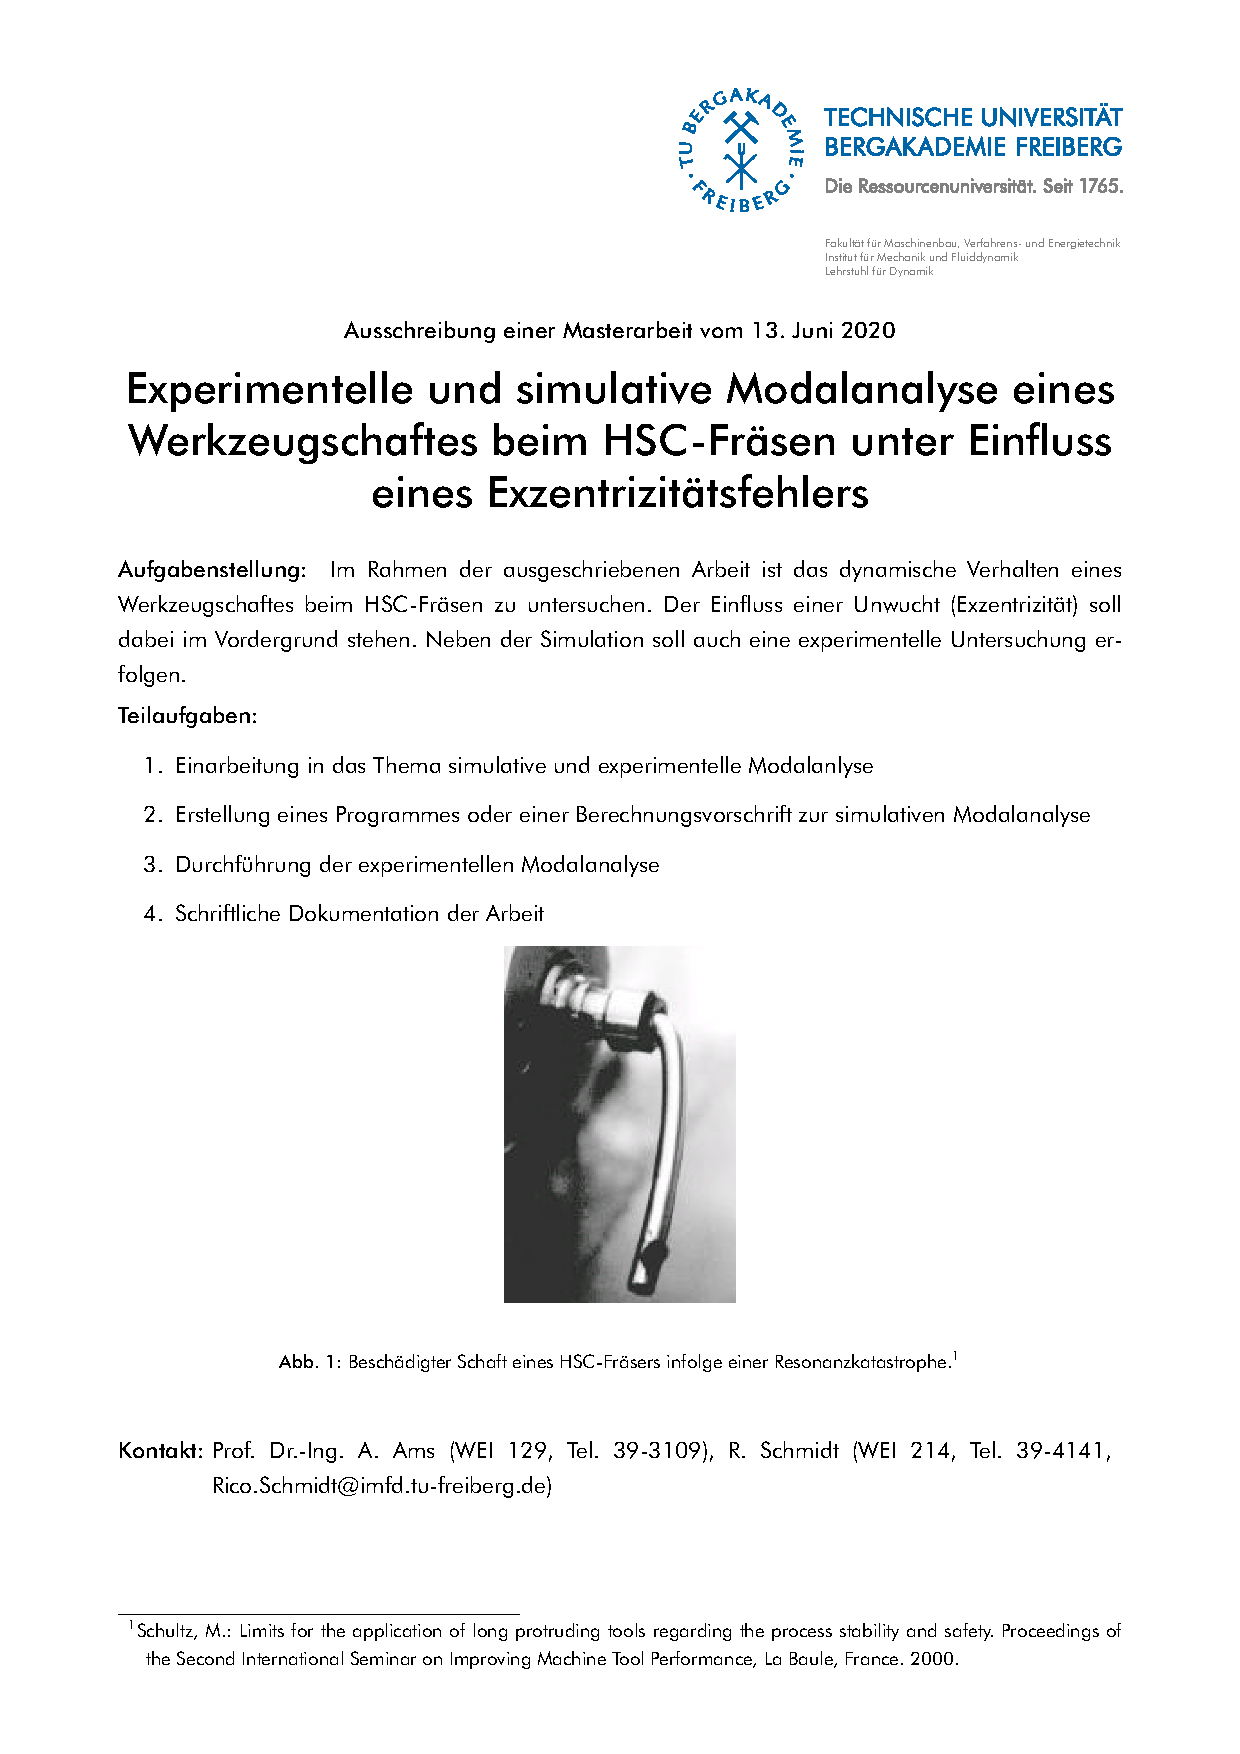
\includepdf[offset=0.8cm 0cm,scale=0.9]{Ausschreibung_Schaukasten.pdf}
	
		%% empty page %%%%%%%%%%%%%%%%%%%%%%%%%%%%%%%%%%%%%%%%%%
	\newpage
	\pagestyle{empty}
	\ \\
	\newpage
	%%%%%%%%%%%%%%%%%%%%%%%%%%%%%%%%%%%%%%%%%%%%%%%%%%%%%%%%%
	
% Contents %%%%%%%%%%%%%%%%%%%%%%%%%%%%%%%%%%%%%%%%%%%%%%%%%%%%%%%%%%%%%%%%%%%%%%%%%%%%%%%%%%%%%
	\pagestyle{fancy}
	\tableofcontents
	
	
%% empty page %%%%%%%%%%%%%%%%%%%%%%%%%%%%%%%%%%%%%%%%%%
		%% empty page %%%%%%%%%%%%%%%%%%%%%%%%%%%%%%%%%%%%%%%%%%
	\newpage
	\pagestyle{empty}
	\ \\
	\newpage
	%%%%%%%%%%%%%%%%%%%%%%%%%%%%%%%%%%%%%%%%%%%%%%%%%%%%%%%%%
	
%%%%%%%%%%%%%%%%%%%%%%%%%%%%%%%%%%%%%%%%%%%%%%%%%%%%%%%%%%%%%%%%%%%%%%%%%%%%%%%%%%%%%%%%%%%%%%%
	
	\fancyhead[LO,RE]{\changefont \nouppercase\leftmark} % Kopfzelle ungrade Seite rechts und gerade Seite links - show section
	
	\pagenumbering{arabic}
	\setcounter{page}{1} 
	
		\pagestyle{fancy}
	\section{Einleitung}\label{sec:einleitung}
	Eine wichtige Fertigungstechnologie in der Metallverarbeitung ist das Hochgeschwindigkeitszerspanen (englisch \textit{High Speed Cutting}, HSC). Dabei handelt es sich um ein fortschrittliches Zerspanungsverfahren, welches hohe Effizienz, Qualität und geringen Verbrauch kombiniert. Eine Reihe von Problemen, die bei herkömmlichen Zerspanungsverfahren auftreten, wurden durch die Anwendung von HSC reduziert. Im Vergleich zum herkömmlichen Zerspanen werden die Schnittgeschwindigkeit und die Vorschubgeschwindigkeit um mehrere Stufen erhöht.\\
	
	Mit zunehmender Schnittgeschwindigkeit nimmt die Abtragsrate pro Zeiteinheit zu, die Schnittzeit nimmt ab und die Verarbeitungseffizienz steigt. Dadurch wird der Herstellungszyklus des Produkts verkürzt und die Wettbewerbsfähigkeit auf dem Markt verbessert. Gleichzeitig verringert eine geringe Schnittmenge mit schneller Bewegungen den Werkzeugverschleiß. Gleichzeitig werden die Schnittkraft und die thermische Spannungsverformung des Werkstücks verringert. Das führt auf bessere Verarbeitungsmöglichkeiten von Teilen und Materialien mit geringer Steifigkeit sowie dünnwandige Teile. Aufgrund der Verringerung der Schnittkraft und der Erhöhung der Drehzahl ist die Arbeitsfrequenz des Schneidsystems weit von der Eigenfrequenz niedriger Ordnung der Werkzeugmaschine entfernt, wodurch die Oberflächenrauheit verringert wird. Die Oberflächenrauheit des Werkstücks ist am empfindlichsten gegenüber der Frequenz niedriger Ordnung. Die HSC-Technologie kann in Anwendungsgebieten eingesetzt werden, die eine hohe Anforderungen an Zerspanleistung und eine hohe Oberflächenqualität erfordern, also insbesondere in der Werkzeugbearbeitung und der Formenbearbeitung. Zum Beispiel gibt es komplexe dreidimensionale Formen, welche höchste Maßgenauigkeit und Oberflächengenauigkeit aufweisen müssen \cite{huseynov2015entwicklung}. \\
	
	Wegen der Frequenzempfindlichkeit des Zerspanungsverfahrens sind die Eigenfrequenzen des Werkzeugs wichtige Parameter. Deshalb wird die Modalanalyse verwendet, um die dynamischen Eigenschaften von Systemen im Frequenzbereich zu untersuchen. Die Eigenfrequenzen sind im konstruktiven Ingenieurbau sehr wichtig, da es unerlässlich ist, dass diese nicht mit den erwarteten Erregungsfrequenzen übereinstimmen (Resonanz). Falls es trotzdem zur Resonanz kommt, kann das Objekts strukturellen Schaden erleiden. Aus methodologischer Sicht ist die Modalanalyse in numerische und experimentelle Modalanalyse zu unterteilen. In dieser Arbeit wird die numerische Modalanalyse mit der Finite-Elemente-Methode (FEM) und die experimentelle Modalanalyse mit Experimenten betrachtet.\\
	
	Es soll die Auswirkung von Exzentrizitätsfehlern auf die Eigenfrequenzen des Werkzeugschaftes beim HSC-Fräsen durch simulative und experimentelle Modalanalyse analysiert werden. Aufgrund der hohen Geschwindigkeiten des Werkzeughalters wird eine nichtlineare Finite-Elemente-Methode, in Kombination mit dem Prinzip von Hamilton, für die Simulation verwendet. Anschließend wird die FE Simulation mit \Matlab durchgeführt. Im experimentellen Teil wird die sogenannte Anregungshammermethode für die experimentellen Modalanalyse benutzt. Außerdem wird das CAD Programm \SolidWorks zur Darstellung der Bauteilen benutzt, die im Experiment angewendet werden. Schließlich werden die Ergebnisse von Simulation und Experiment verglichen und analysiert.
	
	
%% empty page %%%%%%%%%%%%%%%%%%%%%%%%%%%%%%%%%%%%%%%%%%
		%% empty page %%%%%%%%%%%%%%%%%%%%%%%%%%%%%%%%%%%%%%%%%%
	\newpage
	\pagestyle{empty}
	\ \\
	\newpage
	%%%%%%%%%%%%%%%%%%%%%%%%%%%%%%%%%%%%%%%%%%%%%%%%%%%%%%%%%
%%%%%%%%%%%%%%%%%%%%%%%%%%%%%%%%%%%%%%%%%%%%%%%%%%%%%%%%%%%%%%%%%%%%%%%%%%%%%%%%%%%%%%%%%%%%%%%%%%%%%%%%%%%%%%%%%%

		\pagestyle{fancy}
	
	\section{Theoretische Grundlagen} \label{sec:Theoretische Grundlagen}
	
	\subsection{Grundlagen der Finite-Elemente-Methode}\label{sec:Grundlagen-FEM}
	Die Finite-Elemente-Methode (FEM) ist eine zuverlässige und weitverbreitete numerische Analysemethode. Dabei wird hauptsächlich die lineare Finite-Elemente-Methode verwendet, aufgrund ihrer einfachen Anwendung in vielen Bereichen.\\
	
	Die Grundidee der Finite-Elemente-Methode besteht darin, den kontinuierlichen Lösungsbereich in eine Gruppe von finiten Einheiten zu diskretisieren, die auf bestimmte Weise miteinander verbunden sind. Die Unterteilung der ganzen Lösungsbereich in einfachere Teile hat mehrere Vorteile:
	\begin{itemize}
		\item Darstellung von komplexen Geometrien,
		\item Einbeziehung unterschiedlicher Materialeigenschaften,
		\item Einfache Darstellung der Gesamtlösung,
		\item Erfassung von lokalen Auswirkungen.
	\end{itemize}

	Da die Elemente verschieden kombiniert und selbst unterschiedliche Formen haben können, ist es möglich, eine Lösungsdomäne mit komplexen geometrischen Formen zu modellieren. Ein weiteres wichtiges Merkmal der Finite-Elemente-Methode ist die Verwendung von angenommenen Näherungsfunktionen, um die unbekannte Feldfunktion darzustellen, die in der vollständigen Lösungsdomäne gesucht wird. Die Näherungsfunktion im Element wird normalerweise durch den Wert der unbekannten Feldfunktion oder ihre Ableitung an jedem Knoten des Elements und ihre Interpolationsfunktion ausgedrückt. Auf diese Weise wird der Wert der unbekannten Feldfunktion oder ihrer Ableitung an jedem Knoten zur Unbekannten (d.h. zum Freiheitsgrad). Damit wird ein kontinuierliches Problem mit unendlich vielen Freiheitsgraden  zu einem diskreten Problem mit endlich vielen Freiheitsgraden umgesetzt \cite{schwarz2013methode}. \\
	
	Sobald die Unbekannten bestimmt sind, kann der Näherungswert der Feldfunktion in jedem Element durch die Interpolationsfunktion berechnet werden, um die Näherungslösung in der gesamten Lösungsdomäne zu erhalten. Offensichtlich nimmt die Genauigkeit der Lösung weiter zu, wenn die Anzahl der Elemente zunimmt oder wenn die Freiheitsgrade je Element zunehmen. Wenn das Element die Konvergenzanforderungen erfüllt, konvergiert die Näherungslösung schließlich zur exakten Lösung \cite{kattan2010matlab}.
	
	\subsubsection{Nichtlineare Finite-Element-Berechnungen}\label{sec:n.lin_FEM}
	Im Wesentlichen sind alle Probleme der Festkörpermechanik nichtlinear, und es gibt nur wenige analytische Lösungen. Probleme der linearen elastischen Mechanik sind nur eine vereinfachte Annahme der praktischen Probleme. Bei der Finite-Elemente-Analyse umfassen die Annahmen der Linearisierung normalerweise Folgendes:
	\begin{enumerate}
		\item die Knotenverschiebung ist ein kleiner Betrag;
		\item das Material ist linear elastisch;
		\item die Eigenschaften der Randbedingungen sind unverändert während der Bewegung oder Verformung des Körpers.
	\end{enumerate}
	Wenn eine der oben genannten drei Annahmen nicht erfüllt ist, handelt es sich um ein nichtlineares Problem.
	In Anbetracht dessen werden nichtlineare Probleme in der Festkörpermechanik im Allgemeinen in drei Kategorien unterteilt, nämlich Materialnichtlinearität, geometrische Nichtlinearität und Nichtlinearität der Randbedingungen.
	
	\subsubsection{Geometrische Nichtlinearität}\label{sec:geo-n.lin}
	Geometrisch nichtlineare Probleme beziehen sich häufig auf große Verschiebungen oder große Dehnungen innerhalb der Struktur.  Ein Sonderproblem stellen große Verschiebung (wie Translation oder Rotation) mit gleichzeitig kleinen Dehnung dar \cite{rust2011nichtlineare}. In dieser Arbeit dreht der Werkzeugschaft mit hoher Rotationsgeschwindigkeit und Exzentrizität, wodurch nichtlineare Verzerrungen  (nach Green-Lagrange) berücksichtigt werden. Das Materialverhalten soll jedoch als linear elastisch angenommen werden \\
	
	\begin{figure}[H]
		\centering
		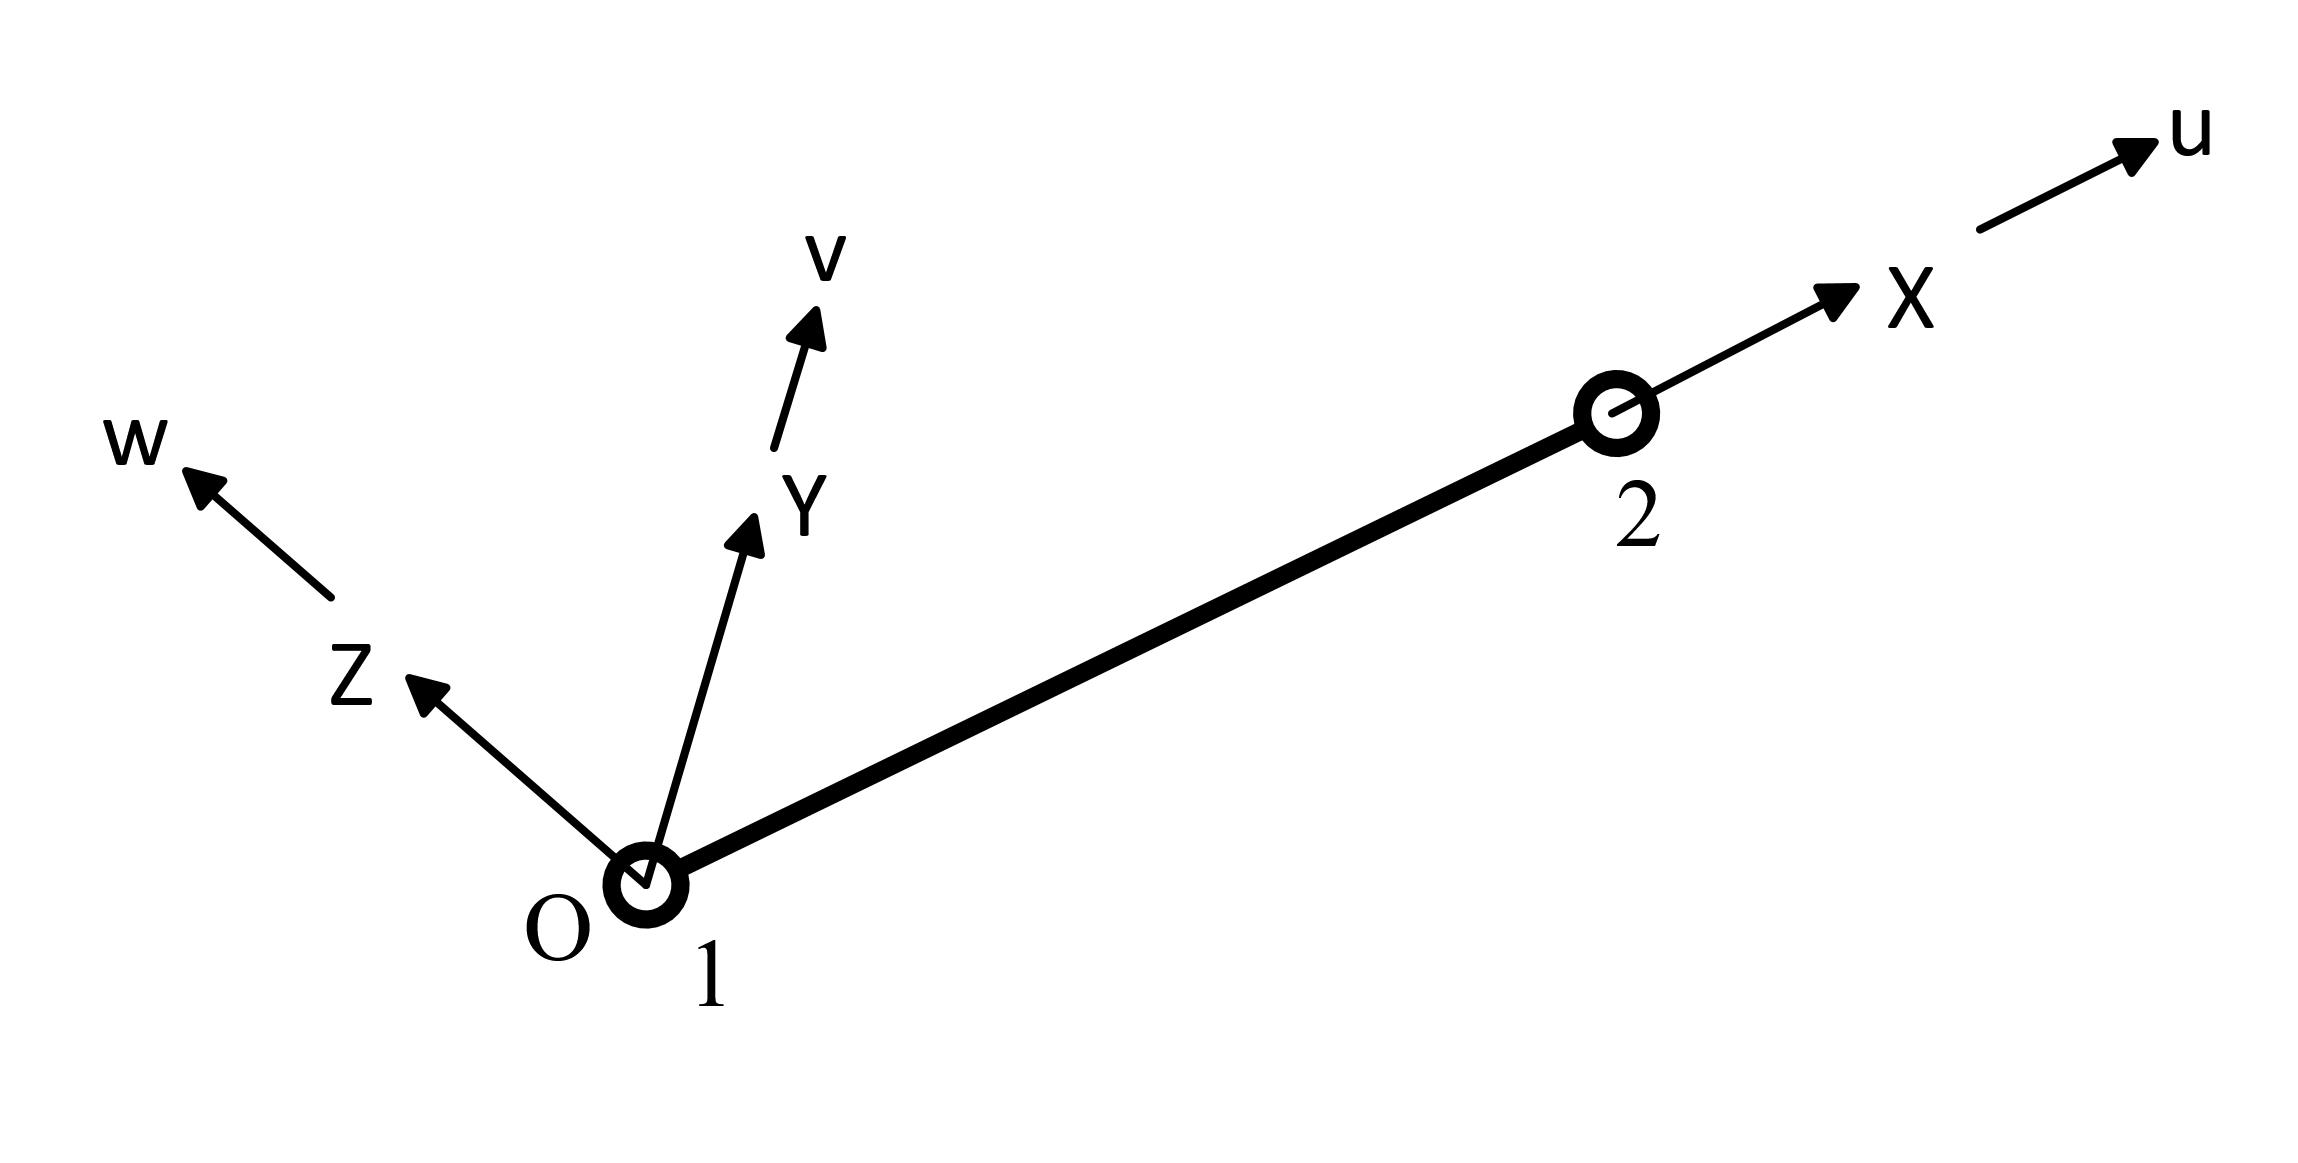
\includegraphics[width=0.74\linewidth, height=0.23\textheight]{Theoretische_Grundlagen/2_Knote_Element}
		\caption{Zweiknotiges Balkenelement mit Koordinaten und Verschiebungen.}
		\label{fig:2-Knote-Element-Koordinate}
	\end{figure}
	
	In Abbildung \ref{fig:2-Knote-Element-Koordinate} ist ein zweiknotiges Balkenelement dargestellt. Weiterhin sind die Verschiebungen $ u $, $ v $ und $ w $ eingetragen. Dabei ist $ u $ die Längsverschiebung und $ v $ sowie $ w $ die Durchbiegungen. Die Green-Lagrange-Dehnungen basieren auf der Änderung des Abstands zwischen zwei benachbarten Punkten. Die genannte Veränderung des Balkens (verformte Länge $ l $, unverformte Länge $ l_{0} $) kann mit
	
	\begin{equation}\label{equ:Änderung der Quadrate}
	\begin{aligned}
	\Delta & = \frac{l^{2}-l_{0}^{2}}{l_{0}^{2}} = \frac{(l_{0}+u)^{2}+v^{2}+w^{2}-l_{0}^{2}}{l_{0}^{2}} = \frac{l_{0}^{2}+2l_{0}u+u^{2}+v^{2}+w^{2}-l_{0}^{2}}{l_{0}^{2}} \\
	       & = 2\frac{u}{l_{0}}+\left(\frac{u}{l_{0}}\right)^{2}+\left(\frac{v}{l_{0}}\right)^{2}+\left(\frac{w}{l_{0}}\right)^{2} .
	\end{aligned}
	\end{equation}
	
	beschrieben werden. Beim Übertragung zum finiten Element ergibt sich
	
	\begin{equation}\label{equ:Übergang zum dx bei Dehnung}
	\frac{u}{l_{0}} \rightarrow \frac{\partial u}{\partial x}=u_{x} \quad \mathrm{;} \quad \frac{v}{l_{0}} \rightarrow \frac{\partial v}{\partial x} = v_{x} \quad \mathrm{;}  \quad \frac{w}{l_{0}} \rightarrow \frac{\partial w}{\partial x}=w_{x}
	\end{equation}
	
	und deshalb
	
	\begin{equation}\label{equ:2.-Änderung der Quadrate}
	\Delta = 2 \frac{\partial u}{\partial x} + \left( \frac{\partial u}{\partial x} \right)^{2} + \left( \frac{\partial v}{\partial x} \right)^{2} + \left( \frac{\partial w}{\partial x} \right)^{2} .
	\end{equation}
	
	Für kleine Verformungen ist das Quadrat vernachlässigbar, sodass nur der erste Term erhalten bleibt, der doppelt so hoch ist wie die lineare oder mechanische Dehnung. Deswegen wird die Green-Lagrange-Dehnung in X-Richtung durch die Hälfte der Änderung der Quadrate gegeben:
	
	\begin{equation}\label{equ:Green-Lagrange-Dehnung}
	\varepsilon_{GL} = \frac{\Delta}{2} = \frac{\partial u}{\partial x} + \frac{1}{2} \left( \frac{\partial u}{\partial x} \right)^{2} + \frac{1}{2} \left( \frac{\partial v}{\partial x} \right)^{2} +\frac{1}{2} \left( \frac{\partial w}{\partial x} \right)^{2} = u_{x}+ \frac{1}{2} u_{x}^{2} + \frac{1}{2} v_{x}^{2} + \frac{1}{2} w_{x}^{2} .
	\end{equation}
	
	\subsection{Lösung nichtlinearer Gleichungssysteme}\label{sec:Lösungsverfahren-n.lin_Dgl}
	
	Für die Finite-Elemente-Methode werden die Knotenverschiebungen als unbekannt Grundparameter verwendet. Das mechanische Modell wird im Allgemeinen nach der Finite-Elemente-Diskreti\-sierung, Elementanalyse, Systemgruppierung und Einführung von Randbedingungen in der Form
	
	\begin{equation}\label{equ:Bewegung-GL}
	\mathbf{M}\, \ddot{\vec{x}}+ \mathbf{D}\, \dot{\vec{x}}+ \mathbf{K}\, \vec{x} = \vec{f} \ ,
	\end{equation}
	
	dargestellt. Dabei ist $ \vec{x} $ der unbekannte Knotenverschiebungsvektor und $ \vec{f} $ der äquivalenter Knotenkraftvektor. Sowohl $ \vec{x} $ und $ \vec{f} $ besitzen die Ordnung $n$. $ \mathbf{M} $ , $ \mathbf{D} $ und $ \mathbf{K} $ sind die Massen-, Dämpfungs- und Steifigkeitsmatrix des Systems. Die Steifigkeitsmatrix ist im Allgemeinen eine positiv definite Matrix. \\
	
	Für statische Probleme kann die Gleichung (\ref{equ:Bewegung-GL}) wie folgt
	
	\begin{equation}\label{equ:Einfach-Bewegung-GL}
	\mathbf{K}\, \vec{x} = \vec{f}
	\end{equation}
	
	vereinfacht werden. Bei dynamischen Problemen müssen zusätzlich die Anfangsbedingungen
	
	\begin{equation}\label{equ:Anfangsbedingung-Bewegung-GL}
	\begin{array}{cc}
	\vec{x}|_{t=0}=\vec{x}_{0} & \dot{\vec{x}}|_{t=0}=\dot{\vec{x}}_{0}
	\end{array}
	\end{equation}
	
	für Gleichung (\ref{equ:Bewegung-GL}) beachtet werden.\\
	
	Wenn $ \mathbf{K} $ oder $\vec{f}$ eine Funktion von $ \vec{x} $ und (oder) dessen Zeitableitung ist, dann wird das Problem nichtlinear. Normalerweise können die nichtlineare Gleichungen nicht direkt gelöst werden. Sie können durch eine Reihe linearer algebraischer Gleichungen angenähert werden, sodass das Lösungsverfahren komplizierter und zeitaufwendiger ist. Es gibt viele Linearisierungsmethoden, z.B. \textsc{Newton}-\textsc{Raphson}-Verfahren \cite{rust2011nichtlineare}, Quasi-\textsc{Newton}-Verfahren \cite{luenberger1984linear}, Modifiziert-\textsc{Newton}-Verfahren, das BFGS-Verfahren und das DFP-Verfahren \cite{matthies1979solution}. In dieser Arbeit wird \textsc{Newton}-\textsc{Raphson}-Verfahren benutzt.\\
	
	Das \textsc{Newton}-\textsc{Raphson}-Verfahren wird mechanisch als Tangentensteifigkeitsmethode bezeichnet und ist eine der bekanntesten Methoden zur Lösung der nichtlinearen Gleichungen. Zur Vereinfachung der Beschreibung kann die Gleichung (\ref{equ:Einfach-Bewegung-GL}) wie folgt umgeschrieben werden:
	
	\begin{equation}\label{equ:Newton-Vereinfach-Bewegung-GL}
	\vec{\varPsi}(\vec{x}) = \mathbf{K}(\vec{x}) \cdot \vec{x}-\vec{f}=\vec{0} \ .
	\end{equation}
	
	Dabei ist $ \vec{\varPsi} $ eine stetige ableitbare Funktion mit dem Näherungsanfangsvektor $ \vec{x}^{(0)} $ und dem Näherungsvektor nach der $n$-ten Iteration ist $ \vec{x}^{(n)} $. Nach der Taylorreihenentwicklung von $ \vec{\varPsi} $ werden die linearen Terme beibehaltet und die Terme höheren Ordnung ignoriert, sodass sich
	
	\begin{equation}\label{equ:Taylorreihe-Newton-Vereinfach-Bewegung-GL}
	\vec{\varPsi}(\vec{x}^{(n)}) = \mathbf{K}_{\text{T}}^{(n)} (\vec{x}-\vec{x}^{(n)})\approx 0
	\end{equation}
	
	ergibt. Mit der Lösung aus Gleichung (\ref{equ:Taylorreihe-Newton-Vereinfach-Bewegung-GL}) kann ein neuer Näherungsvektor mit
	
	\begin{equation}\label{equ:Naeherungswert-x(n+1)}
	\vec{x}^{(n+1)} = \vec{x}^{(n)} - \left( \mathbf{K}_{\text{T}}^{(n)} \right)^{-1} \cdot \vec{\varPsi}(\vec{x}^{(n)}) \ .
	\end{equation}
	
	 berechnet werden. Tie Tangentensteifigkeitsmatrix der Struktur
	
	\begin{equation}\label{equ:Taylorreihe-K}
	\mathbf{K}_{\text{T}}^{(n)} = \left. \dfrac{\partial \vec{\varPsi}}{\partial \vec{x}}\right| _{\vec{x}=\vec{x}^{(n)}}
	\end{equation}
	
	 besteht aus einem Zusammenbau der Tangentensteifigkeitsmatrizen der entsprechenden Elemente. Durch Vergleichen des relativen Fehlers mit dem Ergebnis des vorherigen Iterationsschritts kann der Konvergenzprozess gesteuert werden.\\
	 
	 Deshalb kann der Lösungsmethode von \textsc{Newton}-\textsc{Raphson}-Verfahren bei Programmierung mit folgender Schritte beschreiben:
	 \begin{enumerate}
	 	\item Anfangswert $ x^{(0)} $ und $ n=0 $ einstellen,
	 	\item Tangentensteifigkeitsmatrizen $ \mathbf{K}_{\text{T}}^{(n)} $ berechnen:
	 	\begin{equation}\label{equ:Tangentensteifigkeitsmatrizen}
	 	\mathbf{K}_{\text{T}}^{(n)} = \left. \dfrac{\partial \vec{\varPsi}}{\partial \vec{x}}\right| _{\vec{x}=\vec{x}^{(n)}} ,
	 	\end{equation}
	 	\item $ \vec{\varPsi}^{(n)} $ berechnen:
	 	\begin{equation}\label{equ:Psi-Berechnen}
	 	\vec{\varPsi}^{(n)} = \vec{\varPsi}(\vec{x}^{(n)}) = \mathbf{K}(\vec{x}^{(n)}) \vec{x}^{(n)}-\vec{f},
	 	\end{equation}
	 	\item Funktion $ \mathbf{K}_{\text{T}}^{(n)} \Delta \vec{x}^{(n)} = -\vec{\varPsi}^{(n)} $ lösen und bekommen:
	 	\begin{equation}\label{equ:Delta-X}
	 	\Delta\vec{x}^{(n)} = - (\mathbf{K}_{\text{T}}^{(n)})^{-1} \vec{\varPsi}^{(n)},
	 	\end{equation}
	 	\item neuer Näherungsvektor berechnen:
	 	\begin{equation}\label{equ:Naeherungswert-(n+1)}
	 	\vec{x}^{(n+1)} = \vec{x}^{(n)} + \Delta\vec{x}^{(n)},
	 	\end{equation}
	 	\item Wenn es konvergiert, endet die Iteration; andernfalls lassen $ n=n+1 $ und noch mit Schritt 2 fortfahren.
	 \end{enumerate}
	 
	 \subsection{Prinzip von Hamilton} \label{sec:prinzip-hamilton}
	 In der Physik ist das Prinzip von \textsc{Hamilton} der Ausdruck des 1833 vom irischen Physiker \textsc{William Hamilton} veröffentlichten Prinzips. Das Prinzip von \textsc{Hamilton} besagt, dass die Dynamik eines physikalischen Systems mittels Variationsrechnung einer einzigen Funktion, der \textsc{Lagrange}-Funktion welche alle physikalischen Informationen über das System und die darauf einwirkenden Kräfte enthält, bestimmt wird. \\
	 
	 Für ein System mit potentieller und kinetischer Energie lautet die \textsc{Lagrange}-Funktion nach \cite{gross2004technische}
	 \begin{equation}\label{equ:lagrange-funktion}
	 L = E_{kin} - E_{pot}.
	 \end{equation}

	 
	 Das Hamilton-Prinzip bietet die Möglichkeit, die Bewegung physikalischer Systeme auszudrücken. Anders als die Differentialgleichungsmethode des \textsc{Newton}'schen Bewegungsgesetzes verwendet diese Methode ein Funktional in Form eines  Zeitintegrals.\\
	 
	 Das Prinzip von \textsc{Hamilton} ist auch ein wichtiges Variationsprinzip in der Elastodynamik. Im Gegensatz zu einem System, das aus starren Körper besteht, haben verformbare Körper unendlich viele Freiheitsgrade. Der Zustand des Systems wird daher durch kontinuierliche Funktionen von Raum und Zeit beschrieben. Das erweiterte Prinzip von \textsc{Hamilton} für solche Körper wird durch
	 \begin{equation}\label{equ:Hamilton}
	 \delta\int_{t_{1}}^{t_{2}} \left( E_{kin}-E_{pot}\right)  \mathrm{d}t + \int_{t_{1}}^{t_{2}} \delta W \mathrm{d}t = 0
	 \end{equation}
	 gegeben.
	 Nacheinander sind also die kinetische Energie $ E_{kin} $ und die potenzielle Energie $ E_{pot} $ des Systems sowie die virtuelle Arbeit $ \delta W $ aller angreifenden potentiallosen Kräfte zu bestimmen \cite{wauer2014kontinuumsschwingungen}.
	 

	
%% empty page %%%%%%%%%%%%%%%%%%%%%%%%%%%%%%%%%%%%%%%%%%
		%% empty page %%%%%%%%%%%%%%%%%%%%%%%%%%%%%%%%%%%%%%%%%%
	\newpage
	\pagestyle{empty}
	\ \\
	\newpage
	%%%%%%%%%%%%%%%%%%%%%%%%%%%%%%%%%%%%%%%%%%%%%%%%%%%%%%%%%
%%%%%%%%%%%%%%%%%%%%%%%%%%%%%%%%%%%%%%%%%%%%%%%%%%%%%%%%%%%%%%%%%%%%%%%%%%%%%%%%%%%%%%%%%%%%%%%%%%%%%%%%%%%%%%%%%%
		\pagestyle{fancy}
	\section{Berechnungsmodell}\label{sec:Berechnungsmodell}
	\subsection{Potentielle und kinetische Energie eines Balkens}\label{sec:E-Berechnung}
	
	In dieser Arbeit wird der Frässchaft als ein einseitig eingespannter und ungedämpfter Balken mit Exzentrizitätsfehler modelliert. Die potentielle Energie in Abhängigkeit der Green-Lagrange-Dehnung $ \varepsilon_{GL} $, der Durchbiegungen $ v $ und $ w $ sowie die Verdrehung $ \phi $ lautet nach \cite{gross2004technische}
	
	\begin{equation}\label{equ:Epot}
	E_{pot} = \dfrac{EA}{2} \underset{(L)}{\int} \varepsilon_{GL}^{2} \ \dx + \dfrac{EI}{2} \underset{(L)}{\int} w_{xx}^{2} \ \dx + \dfrac{EI}{2} \underset{(L)}{\int} w_{xx}^{2} \ \dx + \dfrac{GI_{t}}{2} \underset{(L)}{\int} \phi_{xx}^{2} \ \dx \ .
	\end{equation}
	
	Die kinetische Energie wird durch den Exzentrizitätsfehler $ e $ und die Winkelgeschwindigkeit $ \Omega $ beeinflusst. Wie Abbildung \ref{fig:Ekin-Rotation} zeigt,
	lautet der Ortsvektor eines beliebigen Punkts des Balkens im $ X_{1}Y_{1}Z_{1} $-Koordinatensystem nach \cite{wauer2014kontinuumsschwingungen}
	
	\begin{equation}\label{equ:Vektor-(1)rp}
	_{\left( 1\right) }\vec{r}_{p} = 
	\left[
	\begin{array}{l}
	X+u-Yv_{x}-Zw_{x}\\
	Y+v-Z\phi\\
	Z+w+Y\phi
	\end{array}
	\right] \ .  
	\end{equation}
	
	\begin{figure}[H]
		\centering
		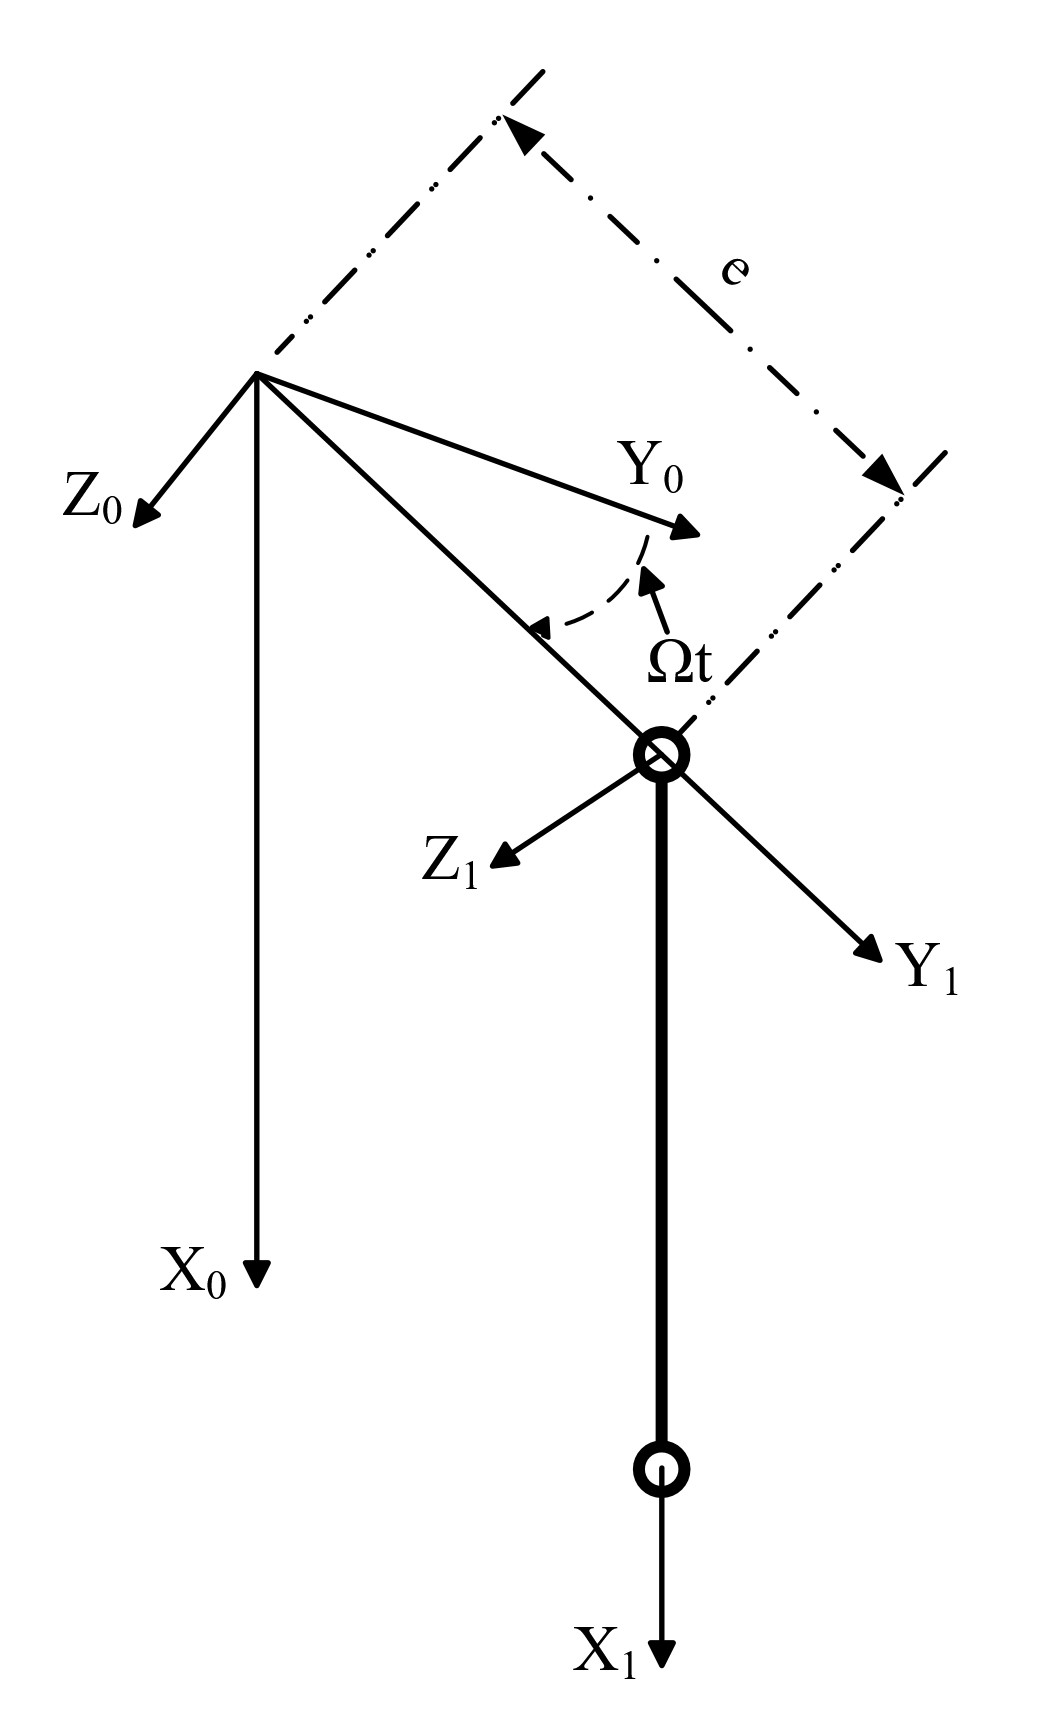
\includegraphics[width=0.45\linewidth, height=0.45\textheight]{Berechnungsmodell/Ekin_Rotation}
		\caption{Balken mit Rotation und Exzentrizitätsfehler.}
		\label{fig:Ekin-Rotation}
	\end{figure}
	
	
	Mit der Rotationsmatrix $ ^{01}\mathbf{R} $ und dem Translationsvektor $ _{(0)}\vec{r}_{12} $ wird der Ortsvektor eines beliebigen Punktes des Balkens im Koordinate $ X_{0}Y_{0}Z_{0} $-Korrdinatensystem mit \cite{heimann2015mechatronik} :
	
	\begin{equation}\label{equ:Vektor-(0)rp}
	%\setlength{\arraycolsep}{2pt}
	_{\left( 0\right) }\vec{r}_{p} = _{\left( 0\right) }\vec{r}_{12} + ^{01}\mathbf{R}\cdot_{\left( 1\right) }\vec{r}_{p} =
	\left[ 
	\begin{array}{c}
	0\\
	e\cdot\cos \Omega t\\
	e\cdot\sin \Omega t
	\end{array}
	\right] +
	\left[  
	\begin{array}{ccc}
	1 & 0 & 0\\
	0 & \cos\Omega t & -\sin\Omega t\\
	0 & \sin\Omega t & \cos\Omega t
	\end{array} 
	\right] \cdot
	\left[
	\begin{array}{l}
	X+u-Yv_{x}-Zw_{x}\\
	Y+v-Z\phi\\
	Z+w+Y\phi
	\end{array}
	\right] 
	\end{equation}
	
	angegeben. Damit ergibt sich die kinetische Energie des Balkens nach \cite{gross2004technische} zu
	
	\begin{equation}\label{equ:Ekin}
	E_{kin} = \dfrac{\rho}{2} \underset{(V)}{\int} \left( \dfrac{\partial _{\left( 0\right) }\vec{r}_{p}}{\partial t} \right)^{2} \ \mathrm{d}V
	= \dfrac{\rho}{2} \underset{(L)}{\int} \underset{(A)}{\int} \left( _{\left( 0\right) }\vec{v}_{p}\right) ^{2} \ \mathrm{d}A \ \dx \ .
	\end{equation}
	
	Mit den folgenden Integralen
	
	\begin{equation}\label{equ:Ekin-Ansatz}
	\setlength{\arraycolsep}{8pt}
	\renewcommand{\arraystretch}{1.3}
	\begin{array}{ll}
	\underset{(A)}{\int} 1 \ \mathrm{d}A = A & \underset{(A)}{\int} Y \ \mathrm{d}A = \underset{(A)}{\int} Z \ \mathrm{d}A = 0\\
	\underset{(A)}{\int} YZ \ \mathrm{d}A =0 & \underset{(A)}{\int} Y^{2} \ \mathrm{d}A = \underset{(A)}{\int} Z^{2} \ \mathrm{d}A = I
	\end{array}
	\end{equation}
	
	lautet die modifizierte kinetische Energie
	\begin{equation}\label{equ:Mod.-Ekin}
	\begin{aligned}
	E_{kin} = \ & \dfrac{\rho A}{2} \underset{(L)}{\int} u_{t}^{2}+e^{2}\Omega^{2}+v^{2}\Omega^{2}+v_{t}^{2}+w^{2}\Omega^{2}+w_{t}^{2}+2ev\Omega^{2}+2ew_{t}\Omega+2vw_{t}\Omega-2v_{t}w\Omega \dx\\
	& +\dfrac{\rho I}{2} \underset{(L)}{\int} v_{xt}^{2}+w_{xt}^{2}+2\Omega^{2}+2\phi^{2}\Omega^{2}+2\phi_{t}^{2}+4\phi_{t}\Omega \dx \ .
	\end{aligned}
	\end{equation}
	
	
	Für die Lösung des Eigenwertproblems des drehenden nichtlinearen Balkens mit Exzentrizitätsfehler wird ein dreidimensionales finites Balkenelement verwendet, wie Bild \ref{fig:2-Knote-Element-Koordinate} gezeigt. Für die Integration und Differentiation der Elemente wird die lokale Koordinate $\xi$ von -1 bis +1 definiert. Die globale Länge eines Elements ist mit $ l_{e} $ gegeben. Der Zusammenhang zwischen lokaler und globaler Koordinate lautet
	\begin{equation}\label{equ:Lokal-zu-global}
	\left. 
	\begin{array}{l}
	\xi (x) = a_{0} + a_{1}x\\
	\xi (x=0) \overset{!}{=} -1\\
	\xi (x=l_{e})  \overset{!}{=} 1
	\end{array} 
	\right\rbrace \Rightarrow 
	\xi = -1 + \frac{2}{l_{e}}x
	\Rightarrow
	\frac{\partial \xi}{\partial x} = \frac{2}{l_{e}}.
	\end{equation}
	
	\subsection{Das dreidimensionale zweiknotige Balkenelement }\label{sec:3D-2.Knote-Balkenelment}
	Bei diesem Element werden die Längsverschiebung $ u $, die Durchbiegungen $ v $ und $ w $ sowie die Verdrehung $ \phi $ durch lineare oder kubische Ansatzfunktionen beschrieben. Für die Längsverschiebung $ u(\xi) $ eines Elements soll der lineare Ansatz
	
	\begin{equation}\label{equ:Linear-Einsatz}
	u(\xi)=a_{0}+a_{1}\xi \ ; \ u(-1) \overset{!}{=} u_{1} \ ; \  u(1) \overset{!}{=} u_{2}
	\end{equation}
	
	verwendet werden. Damit ergibt sich die Längsverschiebung in Vektor-Matrix Schreibweise zu
	
	\begin{equation}\label{equ:Linear-Einsatz-Algebra}
	u(\xi,t) = \vec{N}_{u}(\xi) \vec{u}(t) =
	\left[ \begin{array}{cc}
	\frac{1}{2} - \frac{\xi}{2} & \frac{1}{2} + \frac{\xi}{2}
	\end{array} \right]	
	\left[ 
	\begin{array}{c}
	u_{1}\\
	u_{2}
	\end{array} 
	\right] .
	\end{equation}
	
	Für die Verdrehung $ \phi $ wird auch ein linearer Ansatz analog zur Längsverschiebung verwendet. Deshalb ist die Vektor-Matrix Schreibweise auch identisch. Im Gegensatz dazu wird ein kubischer Ansatz für die Durchbiegung $ w $ mit
	
	\begin{equation}\label{equ:Kubik-Ansatz}
	\begin{array}{c}
	w(\xi) = a_{0} + a_{1}\xi + a_{2}\xi^{2} + a_{3}\xi^{3}\\
	w(-1)\overset{!}{=}w_{1} \ ; \ w_{,\xi}(-1)\overset{!}{=}\varphi_{1} \ ; \ w(+1)\overset{!}{=}w_{2} \ ; \ w_{,\xi}(+1)\overset{!}{=}\varphi_{2} \ .
	\end{array}
	\end{equation}
	
	definiert. Damit kann die Durchbiegung in Vektor-Matrix-Schreibweise mit
	
	\begin{equation}\label{equ:Kubik-Ansatz-Algebra}
	\renewcommand\arraystretch{1.5}
	w(\xi,t) = 
	\vec{N}_{w}(\xi) \vec{w}(t)
	=
	\left[ 
	\begin{array}{c}
	-\frac{1}{16}+\frac{\xi}{16}+\frac{9\xi^{2}}{16}-\frac{9\xi^{3}}{16}\\
	\frac{9}{16}-\frac{27\xi}{16}-\frac{9\xi^{2}}{16}+\frac{27\xi^{3}}{16}\\
	\frac{9}{16}+\frac{27\xi}{16}-\frac{9\xi^{2}}{16}-\frac{27\xi^{3}}{16}\\
	-\frac{1}{16}-\frac{\xi}{16}+\frac{9\xi^{2}}{16}+\frac{9\xi^{3}}{16}
	\end{array}
	\right]^{\mathrm{T}} \cdot
	\left[ 
	\begin{array}{c}
	w_{1}\\
	\varphi_{1}\\
	w_{2}\\
	\varphi_{2}
	\end{array}
	\right]	
	\end{equation}
	
	angegeben werden. Darin kennzeichnen $\varphi_{i}$ die Biegewinkel der Knoten. Für die Durchbiegung $ v $ und dem dazugehörigen Biegewinkel $ \psi $ wird ein identischer Ansatz zu $w$ und $\varphi$ benutzt. Durch die oben genanten Ansätze lautet der Vektor der Knotenvariablen $ \vec{x} $
	
	\begin{equation}\label{equ:Knotenverformung-P}
	\vec{x} = \left[ \left. \ u_{1} \ \right|  \  w_{1} \ \left| \  \varphi_{1} \ \right| \  v_{1} \ \left| \ \psi_{1} \ \right| \ \phi_{1} \ \left| \  u_{2} \ \right| \ w_{2} \ \left| \ \varphi_{2} \ \right|  \  v_{2} \ \left| \  \psi_{2} \ \right| \  \phi_{2} \   \right]^{\mathrm{T}} .
	\end{equation}
	Die Verschiebungen im Element werden durch den Vektor $ \vec{x}_{e}=[ \,u \, | \, w \, | \, v \, | \, \phi \, ] $ beschrieben und ergeben sich nach \cite{steinke2015finite} zu
	
	\begin{equation}\label{equ:Verschiebungen-P-Element}
	\begin{aligned}
	\vec{x}_{e} & =\vec{N}\vec{x} = 
	\left[ 
	\left. \ \vec{N}^{u} \ \right|  \  \vec{N}^{w} \ \left| \  \vec{N}^{v}  \ \right| \ \vec{N}^{\phi} \ \right]^{\mathrm{T}} \vec{x}\\[2mm]
	&= 
	\left[
	\setlength{\arraycolsep}{4pt}
	\begin{array}{llllllllllll} 
	N_{u1} & 0        & 0        & 0        & 0        & 0          & N_{u2} & 0        & 0        & 0        & 0        & 0\\
	0      & N_{w1}   & N_{w2}   & 0        & 0        & 0          & 0      & N_{w3}   & N_{w4}   & 0        & 0        & 0\\
	0      & 0        & 0        & N_{v1}   & N_{v2}   & 0          & 0      & 0        & 0        & N_{v3}   & N_{v4}   & 0\\
	0      & 0        & 0        & 0        & 0        & N_{\phi 1} & 0      & 0        & 0        & 0        & 0        & N_{\phi 1}\\ 
	\end{array}
	\right] \vec{x} \ .
	\end{aligned}
	\end{equation}
	
	Die Ableitung der Formfunktionen $ \vec{N}_{x} $ nach der globalen Variable $ x $ kann durch den Zusammenhang (\ref{equ:Lokal-zu-global}) 
	\begin{equation}\label{equ:X-Ableitung-Formfunktion}
	\vec{N}_{x}(\xi) = \dfrac{\partial \vec{N}(\xi)}{\partial \xi} \cdot \dfrac{\partial \xi}{\partial x} = \dfrac{\partial \vec{N}(\xi)}{\partial \xi} \cdot \dfrac{2}{l_{e}} 
	\end{equation}
	mit berechnet werden
	
	\subsection{Variationsformulierung}\label{sec:Matrizenrechnung}
	In Kapitel (\ref{sec:E-Berechnung}) wurden die kinetische und potenzielle Energie (Gleichungen  \ref{equ:Mod.-Ekin} und \ref{equ:Epot}) schon berechnet. Damit lässt sich das Prinzip von Hamilton (Gleichung \ref{equ:Hamilton})	auswerten. Mit der Annahme, dass für die virtuelle Arbeit der potentiallosen Kräfte $ \delta W=0$ gilt, vereinfacht sich Gleichung \eqref{equ:Hamilton} zu
	
	\begin{equation}\label{equ:Hamilton-mit-Energie-Mod.}
	\int_{t_{1}}^{t_{2}} \delta E_{kin} \, \dt  - \int_{t_{1}}^{t_{2}} \delta E_{pot} \dt = 0.
	\end{equation}
	
	Nach der Variation sowie partiellen Integration ergibt sich die kinetische Energie zu
	\begin{equation}\label{equ:Hamilton-Variation-Partiell-Mod.}
	\begin{aligned}
	\delta E_{kin} = & \rho A \int_{t_{1}}^{t_{2}} \underset{(L)}{\int} -u_{tt}\delta u - v_{tt}\delta v - w_{tt}\delta w - 2v_{t}\Omega \delta w + 2w_{t} \Omega \delta v + v\Omega^{2}\delta v + w\Omega^{2}\delta w  \dx  \dt \\
	& + \rho I \int_{t_{1}}^{t_{2}} \underset{(L)}{\int} -v_{xtt}\delta v_{x} - w_{xtt}\delta w_{x} - 2\phi_{tt}\delta \phi \dx \dt + 2\phi \Omega^{2}\delta \phi  \\
	& + \rho A \int_{t_{1}}^{t_{2}} \underset{(L)}{\int} e\Omega^{2}\delta v \dx \dt
	\end{aligned}
	\end{equation}
	
	und die potenzielle Energie zu
	
	\begin{equation}\label{equ:Epot-mit-Variation}
	\begin{aligned}
	\delta E_{pot} = & \dfrac{EA}{2} \underset{(L)}{\int} \left[ \left( 2u_{x}+3u_{x}^{2}+v_{x}^{2}+w_{x}^{2}+u_{x}^{3}+u_{x}v_{x}^{2}+u_{x}w_{x}^{2}\right) \delta u_{x} \right. \\[1mm]
	& + \left( 2v_{x}u_{x}+v_{x}u_{x}^{2}+v_{x}^{3}+v_{x}w_{x}^{2} \right) \delta v_{x} + \left. \left( 2w_{x}u_{x}+w_{x}u_{x}^{2}+w_{x}v_{x}^{2}+w_{x}^{2} \right) \delta w_{x} \right] \dx  \\[2mm]
	& + EI \underset{(L)}{\int} v_{xx}\delta v_{xx} + w_{xx}\delta w_{xx} \, \dx + EI_{t} \underset{(L)}{\int} \phi_{x}\delta \phi_{x} \, \dx \ .
	\end{aligned}  
	\end{equation}
	
	Wegen der Nichtlinearität wird die variierte potenzielle Energie durch eine Taylorreihe linearisiert. Die linearisierte potenzielle Energie lautet
	\begin{equation}\label{equ:Epot-mit-Taylor-Variation}
	\begin{aligned}
	\Delta \delta E_{pot} & = \dfrac{\partial \delta E_{pot}}{\partial u_{x}}\Delta u_{x} + \dfrac{\partial \delta E_{pot}}{\partial v_{x}}\Delta v_{x} +\dfrac{\partial \delta E_{pot}}{\partial w_{x}}\Delta w_{x} +\dfrac{\partial \delta E_{pot}}{\partial v_{xx}}\Delta v_{xx} +\dfrac{\partial \delta E_{pot}}{\partial w_{xx}}\Delta w_{xx} + \dfrac{\partial \delta E_{pot}}{\partial \phi_{x}}\Delta \phi_{x} \\[2mm]
	& = EA \underset{(L)}{\int} \left[ \left( 1+3u_{x}+\dfrac{3}{2}u_{x}^{2}+\dfrac{1}{2}v_{x}^{2}+\dfrac{1}{2}w_{x}^{2} \right) \Delta u_{x} + \left( v_{x}+v_{x}u_{x} \right) \Delta v_{x} + \left( w_{x}+w_{x}u_{x} \right) \Delta w_{x} \right] \delta u_{x} \dx \\[2mm]
	& \quad + EA \underset{(L)}{\int} \left[ \left( v_{x}+v_{x}u_{x} \right) \Delta u_{x} + \left( u_{x}+\dfrac{1}{2}u_{x}^{2}+\dfrac{3}{2}v_{x}^{2}+\dfrac{1}{2}w_{x}^{2} \right) \Delta v_{x} + \left( v_{x}w_{x} \right) \Delta w_{x} \right] \delta v_{x} \dx \\[2mm]
	& \quad + EA \underset{(L)}{\int} \left[ \left( w_{x}+w_{x}u_{x} \right) \Delta u_{x} + \left( v_{x}w_{x} \right) \Delta v_{x} + \left( u_{x}+\dfrac{1}{2}u_{x}^{2}+\dfrac{1}{2}v_{x}^{2}+\dfrac{3}{2}w_{x}^{2} \right) \Delta w_{x} \right] \delta w_{x} \dx .
	\end{aligned}
	\end{equation}
	
	Die linearisierte potenzielle Energie wird in Gleichung (\ref{equ:Hamilton-mit-Energie-Mod.}) eingesetzt, wodurch
	
	\begin{equation}\label{equ:Hamilton-mit-lin.Energie-Mod.}
	\int_{t_{1}}^{t_{2}} \delta E_{kin} \, \dt  - \int_{t_{1}}^{t_{2}} \Delta\delta E_{pot} \dt = 0
	\end{equation}
	gilt. 
	
	
	\subsection{Diskretisierung}
	Die linearisierte Variationsformulierung aus dem vorherigen Abschnitt wird mit dem FE-Ansatz aus Gleichung \eqref{equ:Verschiebungen-P-Element} diskretisiert. Damit kann die diskretiserte schwache Formulierung der Bewegungsdifferentialgleichung mit
	
	\begin{equation}\label{equ:Schwache-Formulierung-Bewegung-Ggl}
	\begin{aligned}
	0= \ & \rho A \int_{t_{1}}^{t_{2}}\underset{(L)}{\int} [\vec{N}^{u}]^{\mathrm{T}}\vec{N}^{u}\vec{u}_{tt}\delta \vec{u} \, + \,  [\vec{N}^{v}]^{\mathrm{T}}\vec{N}^{v}\vec{v}_{tt}\delta \vec{v} \, + \, [\vec{N}^{w}]^{\mathrm{T}}\vec{N}^{w}\vec{w}_{tt}\delta \vec{w} \, + \, 2\Omega[\vec{N}^{v}]^{\mathrm{T}}\vec{N}^{w}\vec{v}_{t}\delta \vec{w} \\[3mm]
	& - \ 2\Omega[\vec{N}^{w}]^{\mathrm{T}}\vec{N}^{v}\vec{w}_{t}\delta \vec{v} \ - \ \Omega^{2}[\vec{N}^{v}]^{\mathrm{T}}\vec{N}^{v}\vec{v}\delta \vec{v} \ - \ \Omega^{2}[\vec{N}^{w}]^{\mathrm{T}}\vec{N}^{w}\vec{w}\delta \vec{w} \, \dx \dt\\[3mm]
	& + \ \rho I \int_{t_{1}}^{t_{2}}\underset{(L)}{\int} [\vec{N}_{x}^{v}]^{\mathrm{T}}\vec{N}_{x}^{v}\vec{v}_{tt}\delta \vec{v} \ + \ [\vec{N}_{x}^{w}]^{\mathrm{T}}\vec{N}_{x}^{w}\vec{w}_{tt}\delta \vec{w} \ - \ 2\Omega[\vec{N}^{\phi}]^{\mathrm{T}}\vec{N}^{\phi}\vec{\phi}\delta \vec{\phi} \\
	& + \ 2\Omega[\vec{N}^{\phi}]^{\mathrm{T}}\vec{N}^{\phi}\vec{\phi}_{tt}\delta \vec{\phi} \, \dx \dt \ + \ \rho A \int_{t_{1}}^{t_{2}}\underset{(L)}{\int} -e\Omega^{2}[\vec{N}^{v}]^{\mathrm{T}}\delta \vec{v} \, \dx \dt\\[1mm]
	& + \ EA\int_{t_{1}}^{t_{2}}\underset{(L)}{\int} \left[ (1+3u_{x}+\dfrac{3}{2}u_{x}^{2}+\dfrac{1}{2}v_{x}^{2}+\dfrac{1}{2}w_{x}^{2})\vec{N}^{u}_{x}\Delta u \, + \, (v_{x}+v_{x}u_{x})\vec{N}^{v}_{x}\Delta v\right. \\
	& +  \left.  ( w_{x}+w_{x}u_{x} )\vec{N}^{w}_{x}\Delta w\right]^{\mathrm{T}}\vec{N}^{u}_{x} \delta u \, \dx \dt + EA\int_{t_{1}}^{t_{2}}\underset{(L)}{\int} \left[ (u_{x}+\dfrac{1}{2}u_{x}^{2}+\dfrac{3}{2}v_{x}^{2}+\dfrac{1}{2}w_{x}^{2})\vec{N}_{x}^{v}\Delta v \right. \\
	& +  \left. (v_{x}+v_{x}u_{x})\vec{N}_{x}^{u}\Delta u + (v_{x}w_{x})\vec{N}_{x}w\Delta w \right]^{\mathrm{T}} \vec{N}_{x}^{v} \delta v \dx \dt + EA\int_{t_{1}}^{t_{2}}\underset{(L)}{\int} \left[ (w_{x}+w_{x}u_{x})\vec{N}_{x}^{u}\Delta u \right. \\
	& + \left. (v_{x}w_{x})\vec{N}_{x}^{v}\Delta v + (u_{x}+\dfrac{1}{2}u_{x}^{2}+\dfrac{1}{2}v_{x}^{2}+\dfrac{3}{2}w_{x}^{2})\vec{N}_{x}^{w}\Delta w \right]^{\mathrm{T}}\vec{N}_{x}^{w} \delta w \dx \dt .  \\
	\end{aligned}
	\end{equation}
	
	angegeben werden. Die Massenmatrix eines Elements lautet
	
	\begin{equation}\label{equ:Massenmatrix}
	\begin{aligned}
	\mathbf{M}_{e} = & \int_{-1}^{+1} \rho A\left(   [\vec{N}^{u}]^{\mathrm{T}}\vec{N}^{u} + [\vec{N}^{v}]^{\mathrm{T}}\vec{N}^{v} + [\vec{N}^{w}]^{\mathrm{T}}\vec{N}^{w}\right) \\[2mm]
	& + \rho I \left(  [\vec{N}_{x}^{v}]^{\mathrm{T}}\vec{N}_{x}^{v} + [\vec{N}_{x}^{w}]^{\mathrm{T}}\vec{N}_{x}^{w} + 2\Omega[\vec{N}^{\phi}]^{\mathrm{T}}\vec{N}^{\phi}\right)   \dxi,
	\end{aligned}
	\end{equation}
	
	die gyroskopische Matrix
	
	\begin{equation}\label{equ:Gyroskopische-Matrix}
	\mathbf{D}_{e} = \rho A\int_{-1}^{+1} 2\Omega[\vec{N}^{v}]^{\mathrm{T}}\vec{N}^{w} - 2\Omega[\vec{N}^{w}]^{\mathrm{T}}\vec{N}^{v} \dxi
	\end{equation}
	
	und Fliehkraftbelastung
	
	\begin{equation}\label{equ:Fliehkraft}
	\vec{f}_{e} = \rho A\int_{-1}^{+1} -e\Omega^{2}[\vec{N}^{v}]^{\mathrm{T}} \dxi .
	\end{equation}
	
	
	
	Zur Angabe der Steifigkeitsmatrix werden die Ableitungen nach $ \dx $ in $ \mathrm{d}\, \xi $ umgeschrieben mittels
	
	\begin{equation}\label{equ:Zusammenhang-dx-dxi}
	\dfrac{\,\mathrm{d} \, \xi}{\dx}=\dfrac{2}{l_{e}} \Rightarrow \dx=\dfrac{l_{e}}{2}\,\mathrm{d}\, \xi.
	\end{equation}
	
	Damit lautet die Elementsteifigkeitsmatrix
	
	\begin{equation}\label{equ:Steifigkeitsmatrix}
	\begin{aligned}
	\mathbf{K}_{e} = & \ \dfrac{l_{e}}{2} \int_{-1}^{+1} \rho A\left( -\Omega^{2}[\vec{N}^{v}]^{\mathrm{T}}\vec{N}^{v} - \Omega^{2}[\vec{N}^{w}]^{\mathrm{T}}\vec{N}^{w}\right) + \rho I \left( -2\Omega[\vec{N}^{\phi}]^{\mathrm{T}}\vec{N}^{\phi}\right) \\
	& + EA \left\lbrace  \left[ (1+3u_{x}+\dfrac{3}{2}u_{x}^{2}+\dfrac{1}{2}v_{x}^{2}+\dfrac{1}{2}w_{x}^{2})\vec{N}^{u}_{x} + (v_{x}+v_{x}u_{x})\vec{N}^{v}_{x} + (w_{x}+w_{x}u_{x})\vec{N}^{w}_{x}\right]^{\mathrm{T}}\vec{N}^{u}_{x} \right. \\
	& + \left[ (u_{x}+\dfrac{1}{2}u_{x}^{2}+\dfrac{3}{2}v_{x}^{2}+\dfrac{1}{2}w_{x}^{2})\vec{N}_{x}^{v} + (v_{x}+v_{x}u_{x})\vec{N}_{x}^{u} + (v_{x}w_{x})\vec{N}_{x}w \right]^{\mathrm{T}}\vec{N}_{x}^{v}\\
	& + \left. \left[ (w_{x}+w_{x}u_{x})\vec{N}_{x}^{u} + (v_{x}w_{x})\vec{N}_{x}^{v} + (u_{x}+\dfrac{1}{2}u_{x}^{2}+\dfrac{1}{2}v_{x}^{2}+\dfrac{3}{2}w_{x}^{2})\vec{N}_{x}^{w} \right]^{\mathrm{T}}\vec{N}_{x}^{w} \right\rbrace  \ \dxi.
	\end{aligned}
	\end{equation}
	
	Die Größe einer Elementmatrix ist $ 12\times12 $. Für die Elementmassenmatrix werden die Einträge folgendermaßen angegeben
	
	\begin{equation}\label{equ:I.ten-Massenmatrix}
	\renewcommand{\arraystretch}{1.3}
	\mathbf{M}_{ei}=
	\left[ 
	\begin{array}{cccc}
	M_{ei;1,1} & M_{ei;1,2} & \cdots & M_{ei;1,12}\\
	M_{ei;2,1} & M_{ei;2,2} & \cdots & M_{ei;2,12}\\
	\colon     & \colon     & \ddots & \colon\\
	M_{ei;12,1}& M_{ei;12,1}& \cdots & M_{ei;12,12}
	\end{array}
	\right] .
	\end{equation}
	
	Damit kann die Gesamtmassenmatrix nach
	
	\begin{equation}\label{equ:Gesamtmassenmatrix}
	\renewcommand{\arraystretch}{1.4}
	\mathbf{M}=
	\left[ 
	\begin{array}{cccccccc}
	M_{e1;1,1}  & \cdots & M_{e1;1,6}  & M_{e1;1,7}             & \cdots     & M_{e1;1,12}             & 0          &\cdots\\
	\colon      & \ddots & \colon      & \colon                 & \ddots     & \colon                  & \colon     &\cdots\\
	M_{e1;6,1}  & \cdots & M_{e1;6,6}  & M_{e1;6,7}             & \cdots     & M_{e1;6,12}             & 0          &\cdots\\
	M_{e1;7,1}  & \cdots & M_{e1;7,6}  & M_{e1;7,7}+M_{e2;1,1}  & \cdots     & M_{e1;7,12}+M_{e2;1,6}  & M_{e2;1,7} &\cdots\\
	\colon      & \ddots & \colon      & \colon                 & \ddots     & \colon                  & \colon     &\cdots\\
	M_{e1;12,1} & \cdots & M_{e1;12,6} & M_{e1;12,7}+M_{e2;6,1} & \cdots     & M_{e1;12,12}+M_{e2;6,6} & M_{e2;6,7} &\cdots\\
	0           & \cdots & 0           & M_{e2;7,1}             & \cdots     & M_{e2;7,6}              & \ddots     &\cdots\\
	\colon      & \colon & \colon      & \colon                 & \colon     & \colon                  & \colon     &\ddots\\
	\end{array}
	\right] 
	\end{equation}
	
	zusammengebaut werden. Nach gleicher Regel werden auch die Steifigkeitsmatrix und die gyroskopische Matrix des gesamten Systems zusammengebaut. Der gesamte Fliehkraftvektor wird nach 
	
	\begin{equation}\label{equ:Gesamtfliehkraft}
	\vec{f} = \left[ 
	\begin{array}{llllllll}
	f_{e1;1} & \cdots & f_{e1;6} & f_{e1;7}+f_{e2;1} & \cdots & f_{e1;12}+f_{e2;6} & f_{e2;7}+f_{e3;1} & \cdots  
	\end{array} 
	\right]^{\mathrm{T}}
	\end{equation} 
	zusammengebaut. Mit den bereits definierten FE-Ansätzen ergibt sich für statische Probleme  nach Gleichung \ref{equ:Einfach-Bewegung-GL} 
	
	\begin{equation}\label{equ:Einfach-Bewegung-GL-mit-P-F}
	\mathbf{K}\, \vec{x} = \vec{f} \ .
	\end{equation}
	und für dynamische Systeme nach Gleichung \ref{equ:Bewegung-GL}
	
	\begin{equation}\label{equ:Bewegung-GL-mit-Matrizen}
	\mathbf{M}\, \ddot{\vec{x}}+ \mathbf{D}\, \dot{\vec{x}}+ \mathbf{K}\, \vec{x} = \vec{f} \ .
	\end{equation}
	
	\subsection{Zustandsraumdarstellung}
	Durch die Definition der Zustandsgrößen
	
	\begin{equation}\label{equ:Ansatz-in-Systemmatrix}
	\left. 
	\begin{array}{c}
	\vec{z}_{1} = \vec{x} \\
	\vec{z}_{2} = \dot{\vec{x}}
	\end{array}
	\right\rbrace \Rightarrow	
	\begin{array}{l}
	\dot{\vec{z}}_{1} = \vec{z}_{2} \\
	\dot{\vec{z}}_{2} = \ddot{\vec{x}} = - \mathbf{M}^{-1} \cdot \mathbf{K} \cdot \vec{z}_{1} - \mathbf{M}^{-1} \cdot \mathbf{D} \cdot \vec{z}_{2}
	\end{array}
	\end{equation}
	
	kann die Gleichung (\ref{equ:Bewegung-GL-mit-Matrizen}) im Zustandsraum
	
	\begin{equation}\label{equ:1st-Ausgangspunkt}
	\left[ 
	\begin{array}{c}
	\dot{\vec{z}}_{1}\\
	\dot{\vec{z}}_{2}
	\end{array}
	\right] 
	=
	\left[ 
	\begin{array}{cc}
	\mathbf{0}                        & \mathbf{E} \\
	-\mathbf{M}^{-1} \cdot \mathbf{K} & -\mathbf{M}^{-1} \cdot \mathbf{D}
	\end{array}
	\right]
	\cdot
	\left[ 
	\begin{array}{c}
	\vec{z}_{1}\\
	\vec{z}_{2}
	\end{array}
	\right] 
	\end{equation}
	angegeben werden. Es kennzeichnet $\textbf{0}$ die Nullmatrix und $\textbf{E}$ die Einheitsmatrix. Die Eigenfrequenzen der Struktur können durch die Eigenwerte der Systemmatrix
	\begin{equation}\label{equ:Systemmatrix}
	\mathbf{A}
	=
	\left[ 
	\begin{array}{cc}
	\mathbf{0}                        & \mathbf{E} \\
	-\mathbf{M}^{-1} \cdot \mathbf{K} & -\mathbf{M}^{-1} \cdot \mathbf{D}
	\end{array}
	\right]
	\end{equation}
	bestimmt werden.\\
	

	
	
%% empty page %%%%%%%%%%%%%%%%%%%%%%%%%%%%%%%%%%%%%%%%%%
		%% empty page %%%%%%%%%%%%%%%%%%%%%%%%%%%%%%%%%%%%%%%%%%
	\newpage
	\pagestyle{empty}
	\ \\
	\newpage
	%%%%%%%%%%%%%%%%%%%%%%%%%%%%%%%%%%%%%%%%%%%%%%%%%%%%%%%%%
%%%%%%%%%%%%%%%%%%%%%%%%%%%%%%%%%%%%%%%%%%%%%%%%%%%%%%%%%%%%%%%%%%%%%%%%%%%%%%%%%%%%%%%%%%%%%%%%%%%%%%%%%%%%%%%%%%

		\pagestyle{fancy}

	\section{Experimentelle Untersuchungen} \label{sec:Experimentelle Untersuchungen}

	\subsection{Versuchsziel und -planung}\label{sec:Versuchsziel und -planung}
	
	Der Hauptzweck dieses Experiments besteht darin, die Modalanalyse der HSC-Werkzeugschäfte unter Rotation und Exzentrizität durchzuführen. Dafür wurden folgende Teilaufgaben bearbeitet:
	
	\begin{enumerate}
		\item Äquivalente Realisierung der Rotation mit Exzentrizität bei HSC-Schäften.
		\item Festlegung geeigneter Versuchsobjekte (Abmessungen der Probekörper).
		\item Aufbau des Versuchsstands und Durchführung der Messungen.
	\end{enumerate}
	
	Die Messdaten sollen zum Validieren des theoretisch Modells eines rotierenden Schafts mit Exzentrizität dienen. Die Planung kann unterteilt werden in den allgemeinen Messaufbau und die Wahl der Probekörper.
	\\
	Für die Modalanalyse wird zur Erregung ein Impulshammer verwendet. Anschließend wird mit einem Beschleunigungssensor die Antwort gemessen und die Übertragungsfunktion ermittelt. Die Übertragungsfunktion ist mit
	

	
	\begin{equation}\label{equ:Übertragungsfunktion}
	H(\omega)\equiv \dfrac{Y(\omega)}{X(\omega)}
	\end{equation}
	
	gegeben un repräsentiert das komplexe Verhältnis zwischen Ausgang $ Y(\omega) $ und Eingang $ X(\omega) $ als Funktion der	(Kreis-) Frequenz $ \omega $. Die Übertragungsfunktion beschreibt die dynamischen Verhältnisse eines Systems unabhängig von der zur Messung benutzten Signalart \cite{dossing1989strukturen}.\\
	 
	Die Übertragungsfunktion wird dabei für verschiedene Anregungspunkte bestimmt. Diese Versuchsmethode erlaubt es nicht, die experimentelle Modalanalyse unter Rotation durchzuführen, da der Beschleunigungssensor kabelgebunden ist. Aus diesem Grund wird am oberen Ende des Werkzeugschafts eine Radialkraft angebracht. Damit wird die Wirkung der Fliehkraft infolge der Rotation sowie Exzentrizität äquivalent berücksichtigt. Durch die Formänderungsenergie kann der Zusammenhang zwischen die Radialkraft $ F $ und Schwerpunktgeschwindigkeit ($e \Omega$) bestimmt werden. Nach \cite{gross2017technische} lautet die Formänderungsenergie für einen Biegebalken 
	
	\begin{equation}\label{equ:Formanderungsenergie}
	W = \dfrac{1}{2} \int_{0}^{L} \dfrac{M_{b}^{2}(x)}{EI} \dx .
	\end{equation}
	
	Wie die Abbildung \ref{fig:Zusammenhang_Omega_F} gezeigt, für einen Balken mit Rotation und Exzentrizität ergibt sich das Schnittmoment zu
	
	\begin{equation}\label{equ:Biegemoment-Rotation}
	M_{b1}(x) = -\int_{x}^{L} \rho A e \Omega^{2} (\xi-x) \dxi = \rho A e \Omega^{2} \left[ -\dfrac{L^{2}}{2}+Lx-\dfrac{x^{2}}{2}\right] ,
	\end{equation}
	
	womit die Formänderungsenergie wie folgt
	
	\begin{equation}\label{equ:Formanderungsenergie-Rotation}
	W_{1} = \dfrac{1}{2} \int_{0}^{L} \dfrac{M_{b1}^{2}(x)}{EI} \dx = \dfrac{\rho^{2}A^{2}e^{2}\Omega^{4}L^{5}}{40EI}
	\end{equation}
	
	lautet. Beim Balken mit Radialkraft ergibt sich das Schnittmoment zu
	
	\begin{equation}\label{equ:Biegemoment-Radialkraft}
	M_{b2}(x) = F\cdot(x-L)
	\end{equation}
	
	und damit die Formänderungsenergie zu
	
	\begin{equation}\label{equ:Formanderungsenergie-Radialkraft}
	W_{2} = \dfrac{1}{2} \int_{0}^{L} \dfrac{M_{b2}^{2}(x)}{EI} \dx = \dfrac{F^{2}L^{3}}{6EI}.
	\end{equation}
	
	Das Verhältnis zwischen Radialkraft $ F $ und Schwerpunktgeschwindigkeit ($e \Omega$) folgt aus
	\begin{equation}\label{equ:Verhältnis-Rotaion-und-Radialkraft}
	W_{1} \overset{!}{=} W_{2} \,\,\,\,\,\,\,\,\,\Rightarrow F = \pm \dfrac{1}{2} \sqrt{\dfrac{3}{5}} \rho A L e \Omega^{2}.
	\end{equation}
	
	\begin{figure}[H]
		\centering
		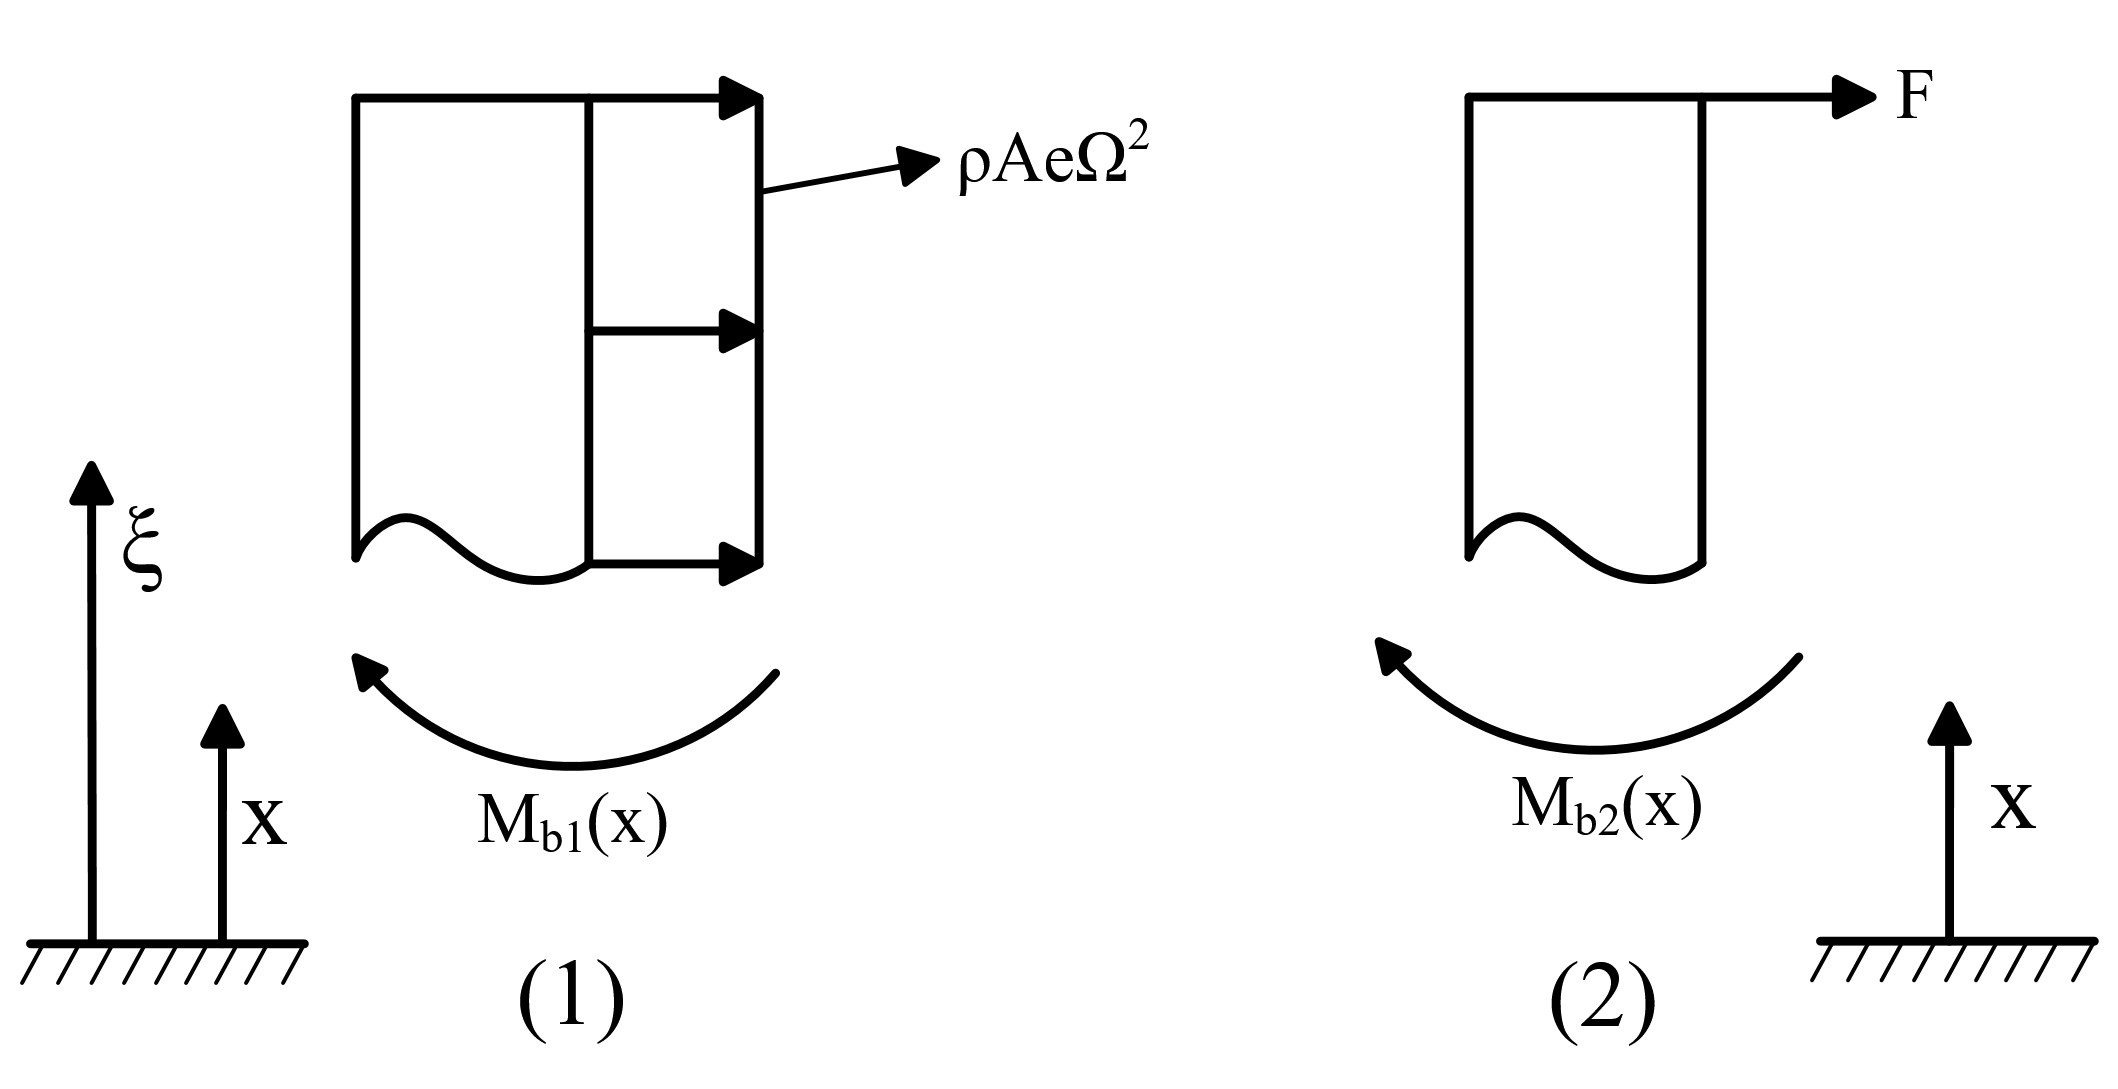
\includegraphics[width=0.85\linewidth, height=0.28\textheight]{Experimentelle_Untersuchungen/Zusammenhang_Omega_F}
		\caption{Schnittmoment für (1) einen Balken mit Rotation und Exzentrizität und (2) einen Balken mit Radialkraft.}
		\label{fig:Zusammenhang_Omega_F}
	\end{figure}
	
	Durch Änderung der Radialkraft können unterschiedliche Werte der Schwerpunktgeschwindigkeit ($e \Omega$) nach Gleichung \ref{equ:Verhältnis-Rotaion-und-Radialkraft} simuliert werden. Die Radialkraft soll dabei mit einer Feder aufgebracht werden, welche die Gesamtsteifigkeit möglichst wenig beeinflusst. Auf die Lagerung des Schaftes und die Verbindung mit der Feder wird später eingegangen \cite{Kokavecz2010}.
	
	\subsection{Versuchsaufbau}\label{sec:Versuchsaufbau}
	
	\subsubsection{Versuchsobjekt}\label{sec:Versuchsobjekt}
	Bei den Versuchen werden HSC-Hohlschäfte mit unterschiedlicher Wandstärke verwendet. Die dazugehörigen Parameter sind in der folgenden Tabelle \ref{tab:Datentabelle-Schaft} zusammengestellt.
	
	\begin{table}[H]\label{tab:Datentabelle-Schaft}
		%\renewcommand\arraystretch{1.2}
		\centering
		%\resizebox{\textwidth}{12mm}{		
		\begin{tabular}{|c|c|c|c|c|c|c|}
			\hline
		    Nr.     & Bezeichnung  & Werkstoff  & \makecell[c]{Aussen-\\durchmesser\\$  [mm] $}  & \makecell[c]{Wand-\\stärke\\$  [mm] $} & \makecell[c]{L/D-\\ Verhältnis} & \makecell[c]{Masse\\$  [g] $}\\
			\hline
		 	1       & Schaft-$ 10\times8 $     & S235J0   & 10          & 1      & 33       & 72,77 \\
			\hline
			2       & Schaft-$ 10\times9  $    & S235J0   & 10          & 0,5    & 33       & 38,41\\
			\hline	 
		\end{tabular}%}
		\caption{Parameter der verwendeten Versuchsschäfte.}
	\end{table}
		Für die Lagerung und Einbringung der Vorspannkraft ist es jedoch notwendig, weitere Bauteilen an den jeweiligen Schaft anzubringen. In Abbildung \ref{fig:Schaft-10x8} ist zunächst die Geometrie der Probe Nr.1 dargestellt. 
	
	\begin{figure}[H]
		\centering
		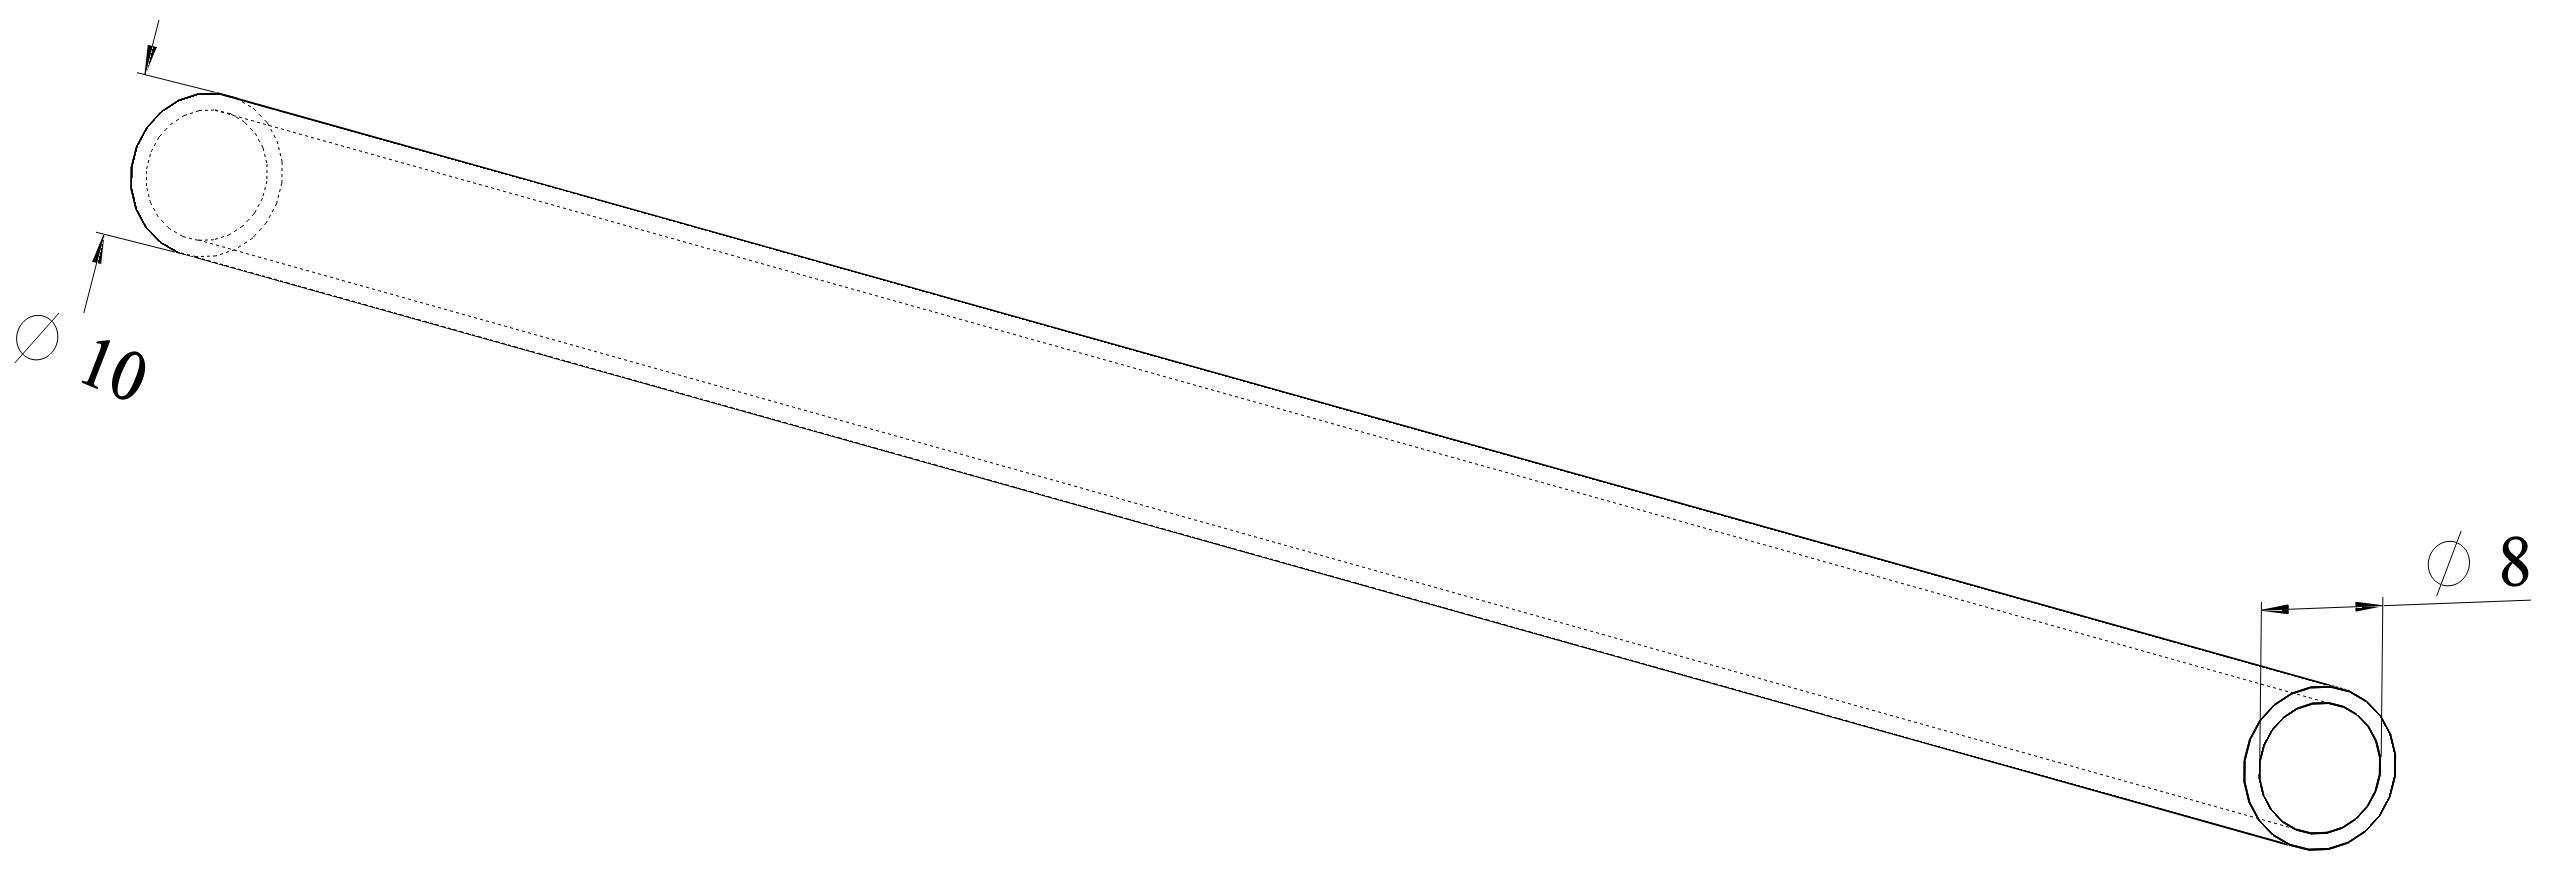
\includegraphics[width=0.9\linewidth, height=0.25\textheight]{Experimentelle_Untersuchungen/Schaft_10x8}
		\caption{3D-Modell von Probekörper Nr.1  (Schaft-$ 10\times8 $).}
		\label{fig:Schaft-10x8}
	\end{figure}

	Dazu wird das untere Ende des Schaftes auf einen Stopfen aufgeschrumpft. Analog dazu wird das obere Ende des Schaftes auf einen Stopfen für die Einbringung der Federkraft aufgeschrumpft. Die beiden Bauteile sind in Abbildung  \ref{fig:Stopfen-Schaft-10x8} dargestellt. \\
	
	Der Stopfen für die Krafteinbringung weist einen Würfeln am freien Ende auf. Dieser dient dazu, den Beschleunigungssensor magnetisch anzuheften. Weiterhin ist eine Gewindebohrung eingebracht, um eine Ringschraube einschrauben zu können. Über diese wird dann die Vorspannkraft mittels Feder eingeleitet. 
	
	
	
	
	\begin{figure}[H]
		\centering
		\begin{minipage}[t]{0.5\linewidth}
			\centering
			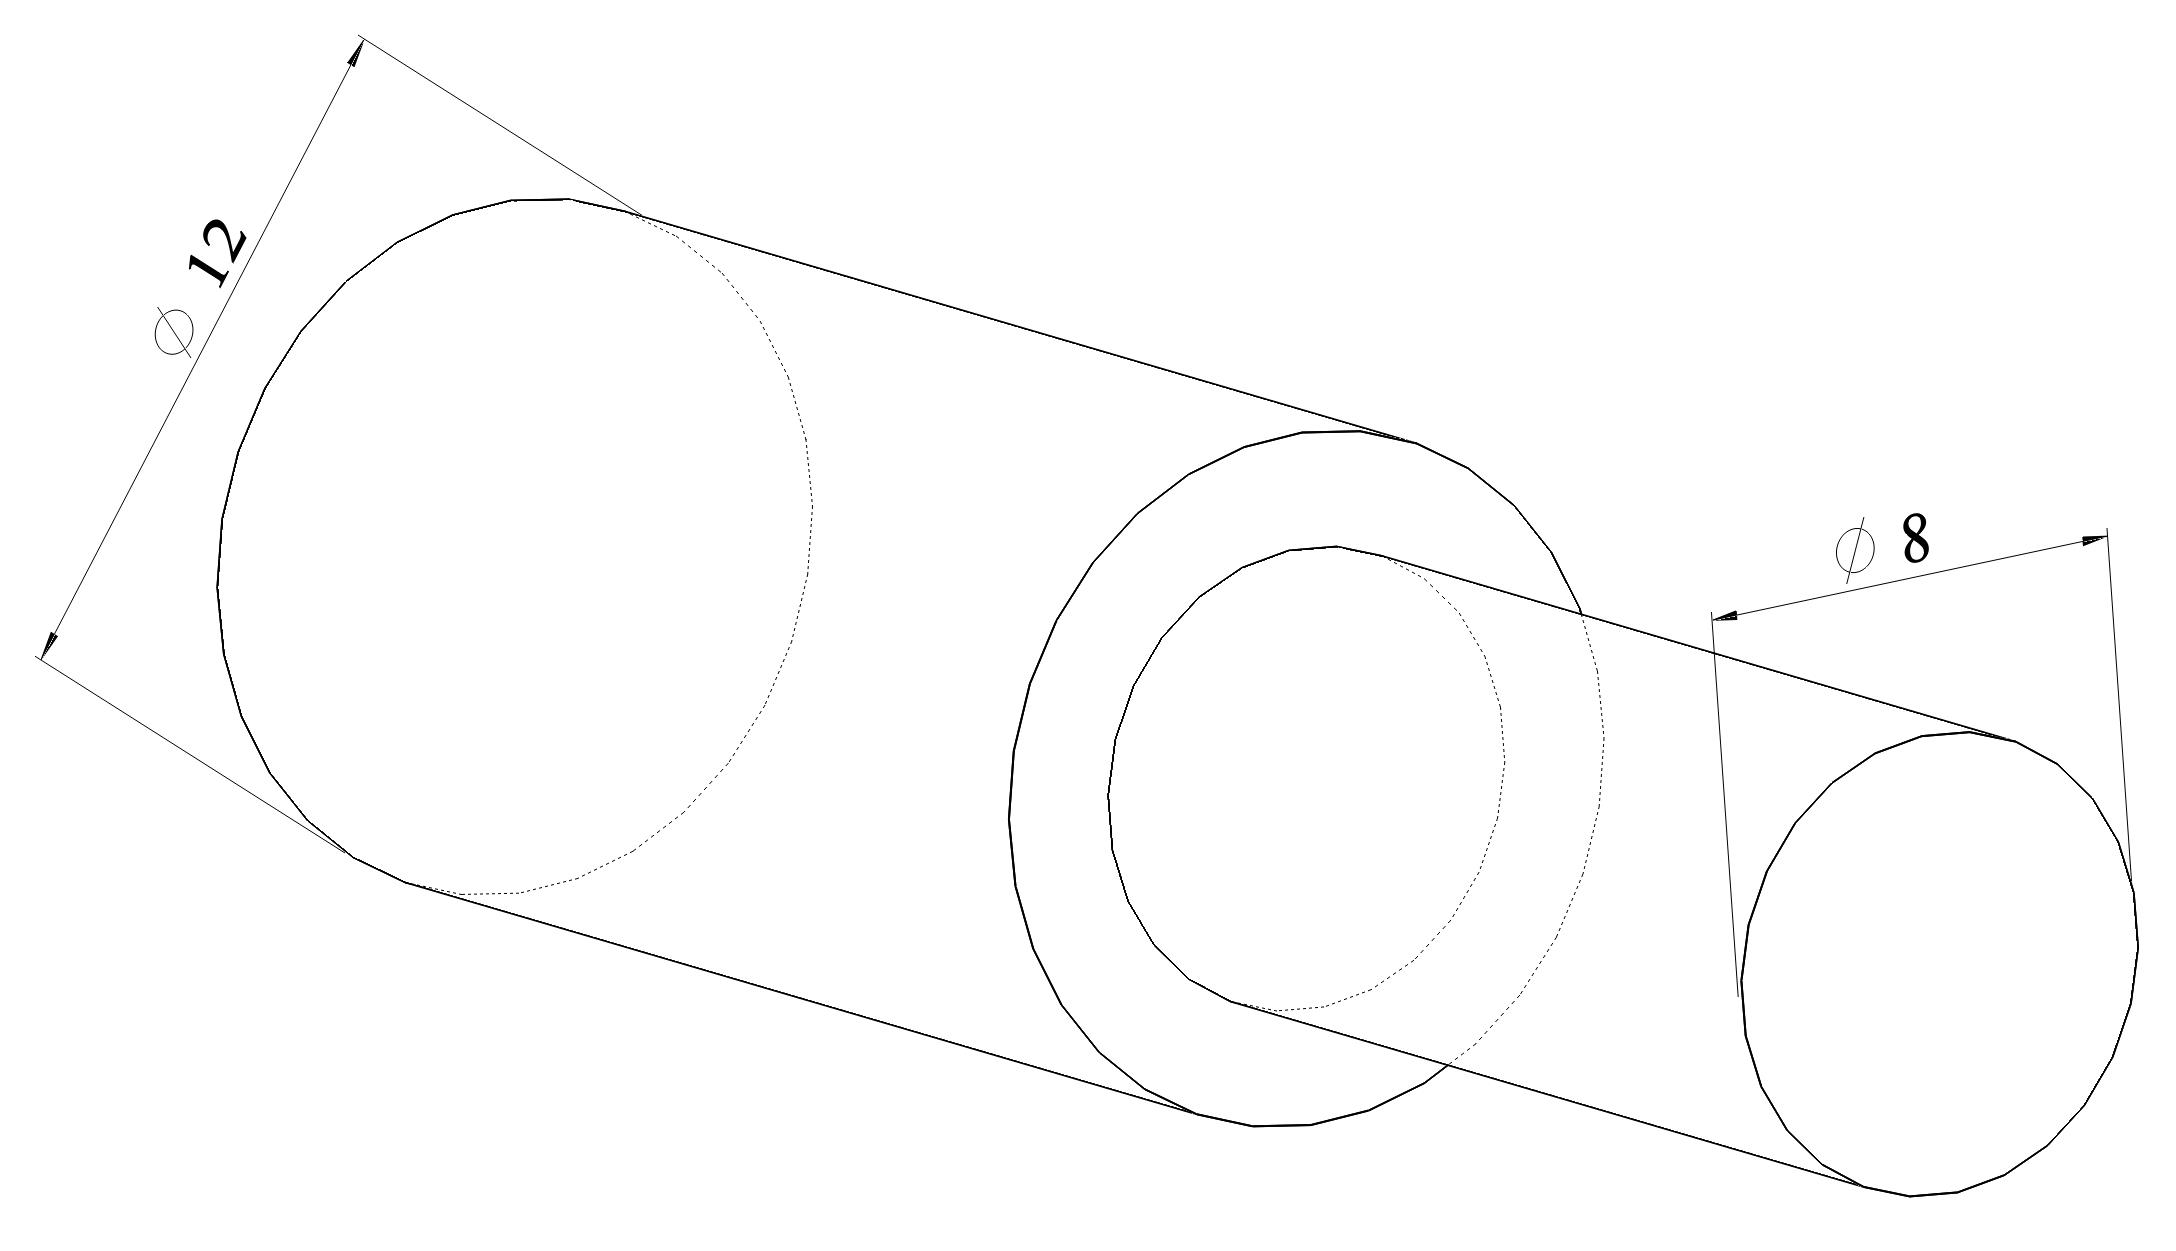
\includegraphics[width=1.0\linewidth, height=0.23\textheight]{Experimentelle_Untersuchungen/10x8_Lagerung_Stopfen}
		\end{minipage}% <- sonst wird hier ein Leerzeichen eingefügt
		\hfill
		\begin{minipage}[t]{0.45\linewidth}
			\centering
			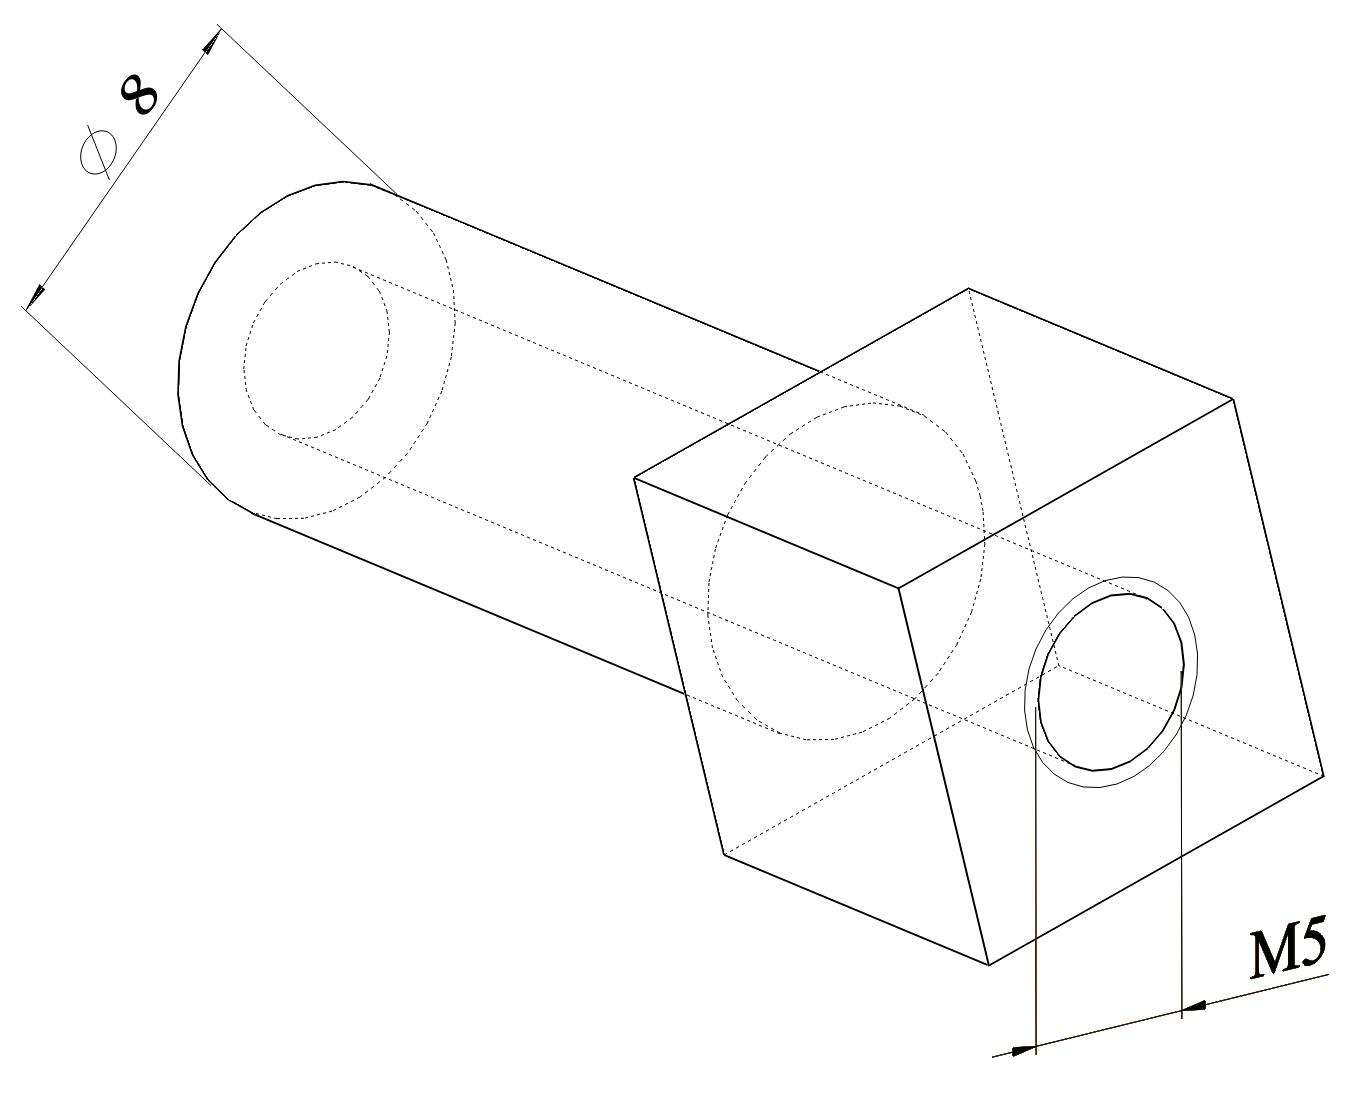
\includegraphics[width=1.0\linewidth, height=0.23\textheight]{Experimentelle_Untersuchungen/10x8_Schraube_Stopfen}
		\end{minipage}
	\caption{3D-Modelle der Stopfen für den Schaft-$ 10\times8 $ für die Lagerung (links) und Einbringung der Vorspannkraft (rechts).}
	\label{fig:Stopfen-Schaft-10x8}
	\end{figure}
	
	
	In Abbildung \ref{fig:Baugruppe-Schaft-10x8} ist nochmals der Zusammenbau der einzelnen Teile zu einer Baugruppe zu sehen. Darin ist auch eine Ringschraube enthalten, über welche die Feder zur Vorspannung eingehängt wird. Die komplette Bauteile (z.B. Aufnahmehaltung und -platte, Gegenkrafthaltung) sind durch die Zeichnungen im Anhang dargestellt.
	
	\begin{figure}[H]
		\centering
		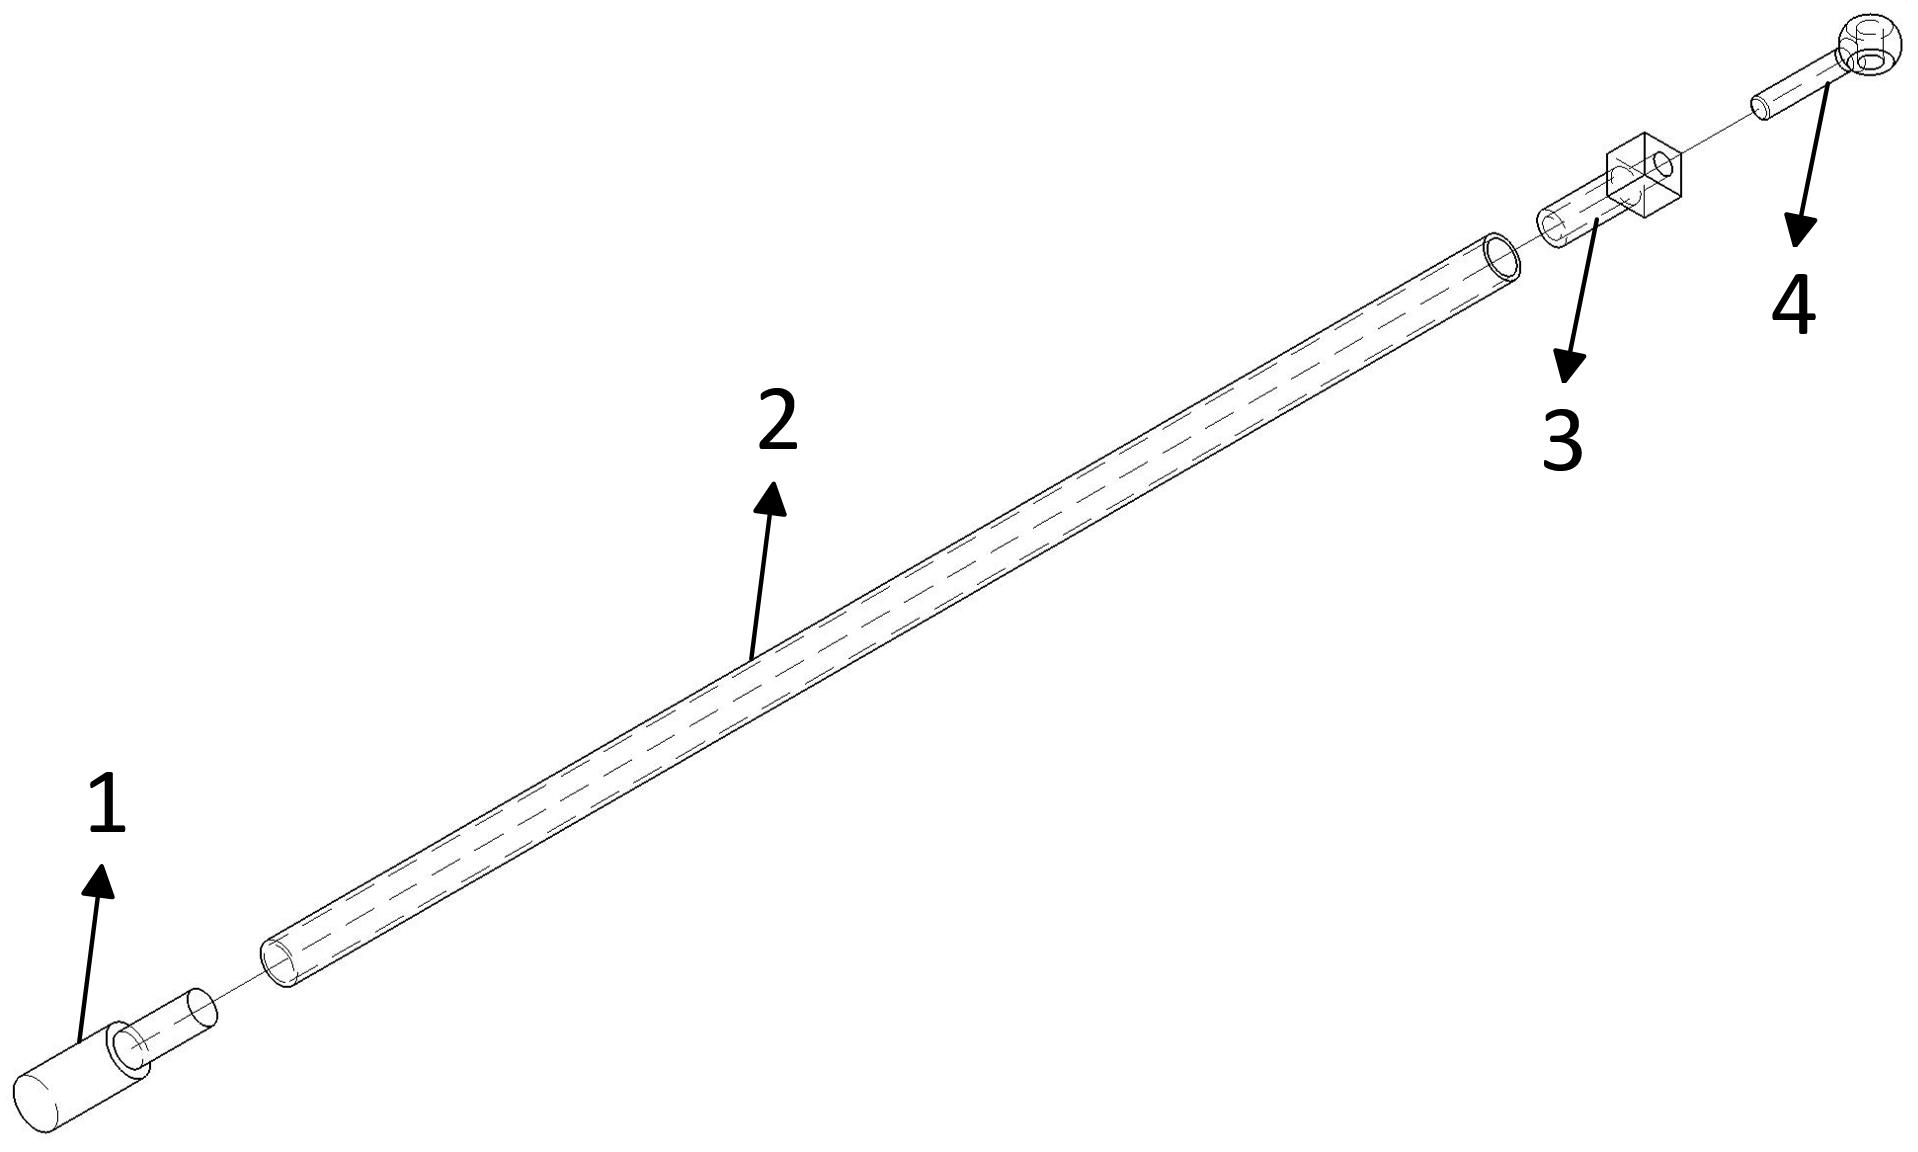
\includegraphics[width=0.85\linewidth, height=0.35\textheight]{Experimentelle_Untersuchungen/Schaft_10x8_Baugruppe}
		\caption{3D-Modell der Baugruppe des Schaftes-$ 10\times8 $ (1: Stopfen Lagerung, 2: Schaft, 3: Stopfen Vorspannkraft, 4: Ringschraube).}
		\label{fig:Baugruppe-Schaft-10x8}
	\end{figure}
	

	
	
	
	\subsubsection{Aufbau des Versuchsstandes}\label{sec:Aufbau des Versuchsstandes}
	
	Die Abbildung \ref{fig:Versuchsaufbau} zeigt die grundsätzlichen Komponenten des Versuchsaufbaus in der Prüfumgebung. Es handelt sich dabei um die folgende Objekte:
	\begin{itemize}
		\item Objekt 1: PC-Monitor mit der Bedienoberfläche von \textsc{PULSE LabShop}, um den Versuchsstatus zu überprüfen.
		\item Objekt 2: Impulshammer, welcher durch Anschlagen der Versuchsprobe die Anregung erzeugt.
		\item Objekt 3: Versuchskörper, wie er bereits in Abbildung \ref{fig:Baugruppe-Schaft-10x8} gezeigt wurde.
		\item Objekt 4: Beschleunigungssensor zur Messung Systemantwort.
		\item Objekt 5: Haltevorrichtung zur Befestigung der Feder.
		\item Objekt 6: Kraftsensor zur Messung der aufgebrachten Vorspannkraft.
		\item Objekt 7: Analog-Digital-Wandler, welcher die aktuelle Vorspannkraft anzeigt.
	\end{itemize}
	
	\begin{figure}[H]
		\centering
		\subfigure{ 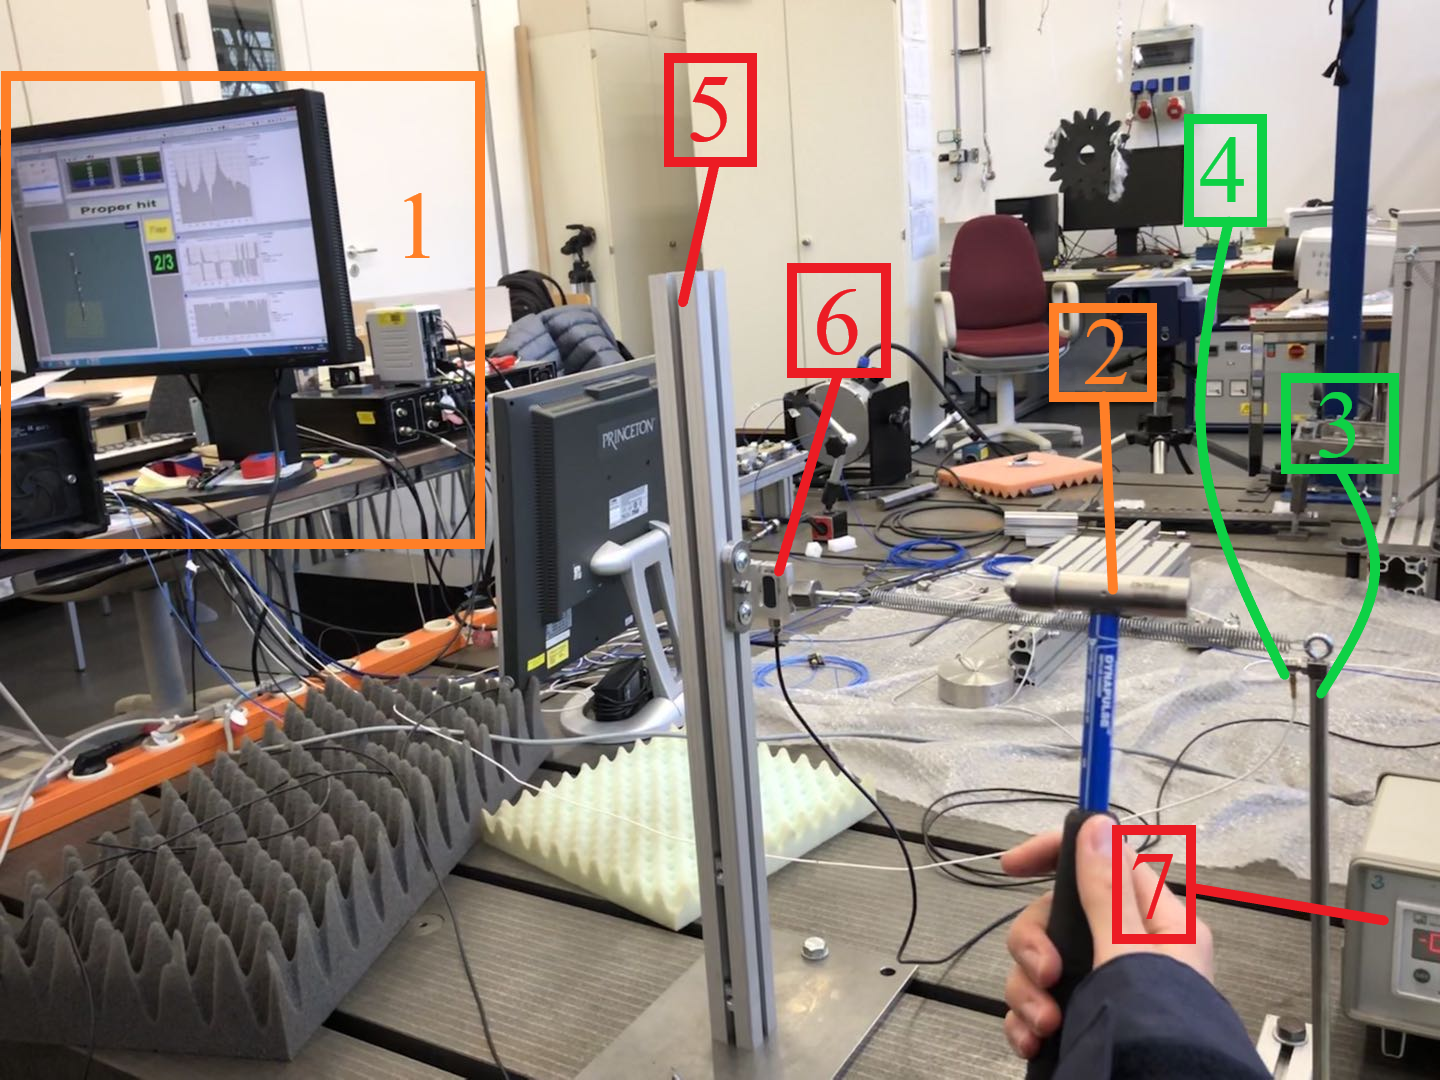
\includegraphics[width=0.48\linewidth, height=0.25\textheight]{Experimentelle_Untersuchungen/Aufbau_Versuchsstand_01.png} }
		\subfigure{ 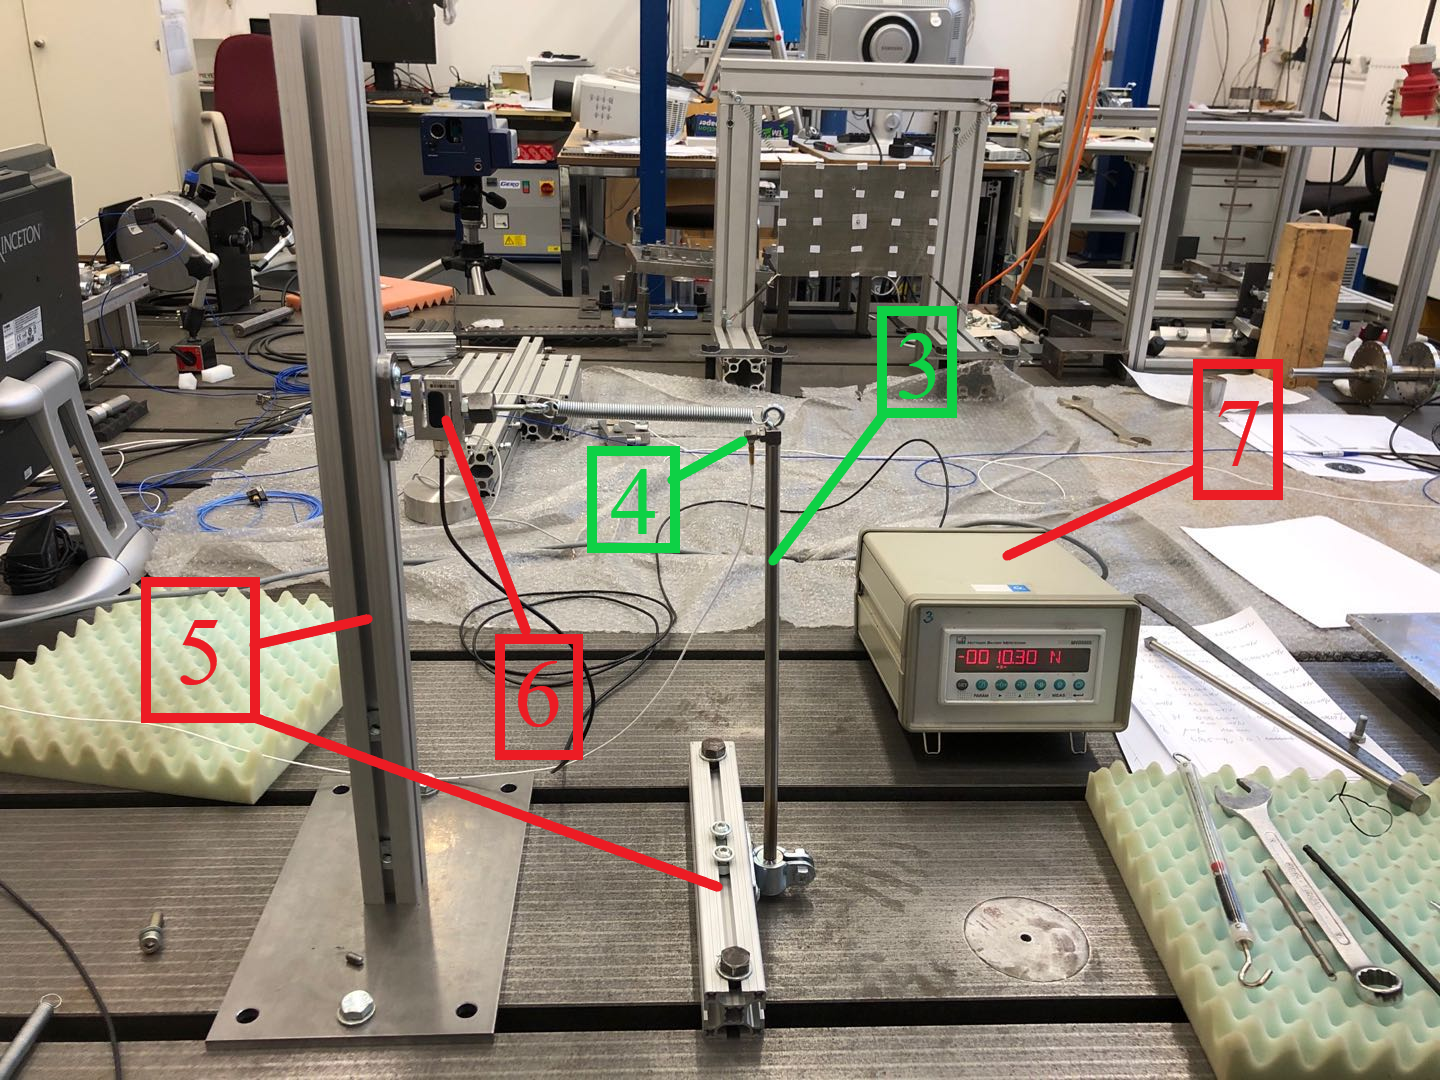
\includegraphics[width=0.48\linewidth, height=0.25\textheight]{Experimentelle_Untersuchungen/Aufbau_Versuchsstand_02.png} }
		\caption{Versuchsaufbau mit einzelnen Objekten.}
		\label{fig:Versuchsaufbau}
	\end{figure}

	
	\subsubsection{Messsoftware}\label{sec:Messsoftware}
	
	In Bezug auf die Messsoftware werden in dieser Arbeit zwei Softwarepakete verwendet. Bei dem ersten handelt es sich um \textsc{PULSE LabShop} von der Firma \textsc{Brüel \& Kj\ae{}r}. Damit werden die Sensorsignale analysiert und für mehrere Messwiederholungen gemittelt. Die für dieses Experiment verwendete Bedienoberfläche von \textsc{PULSE LabShop} ist im Wesentlichen in Abbildung \ref{fig:B&K-Software} dargestellt.
	
	\begin{figure}[H]
		\centering
		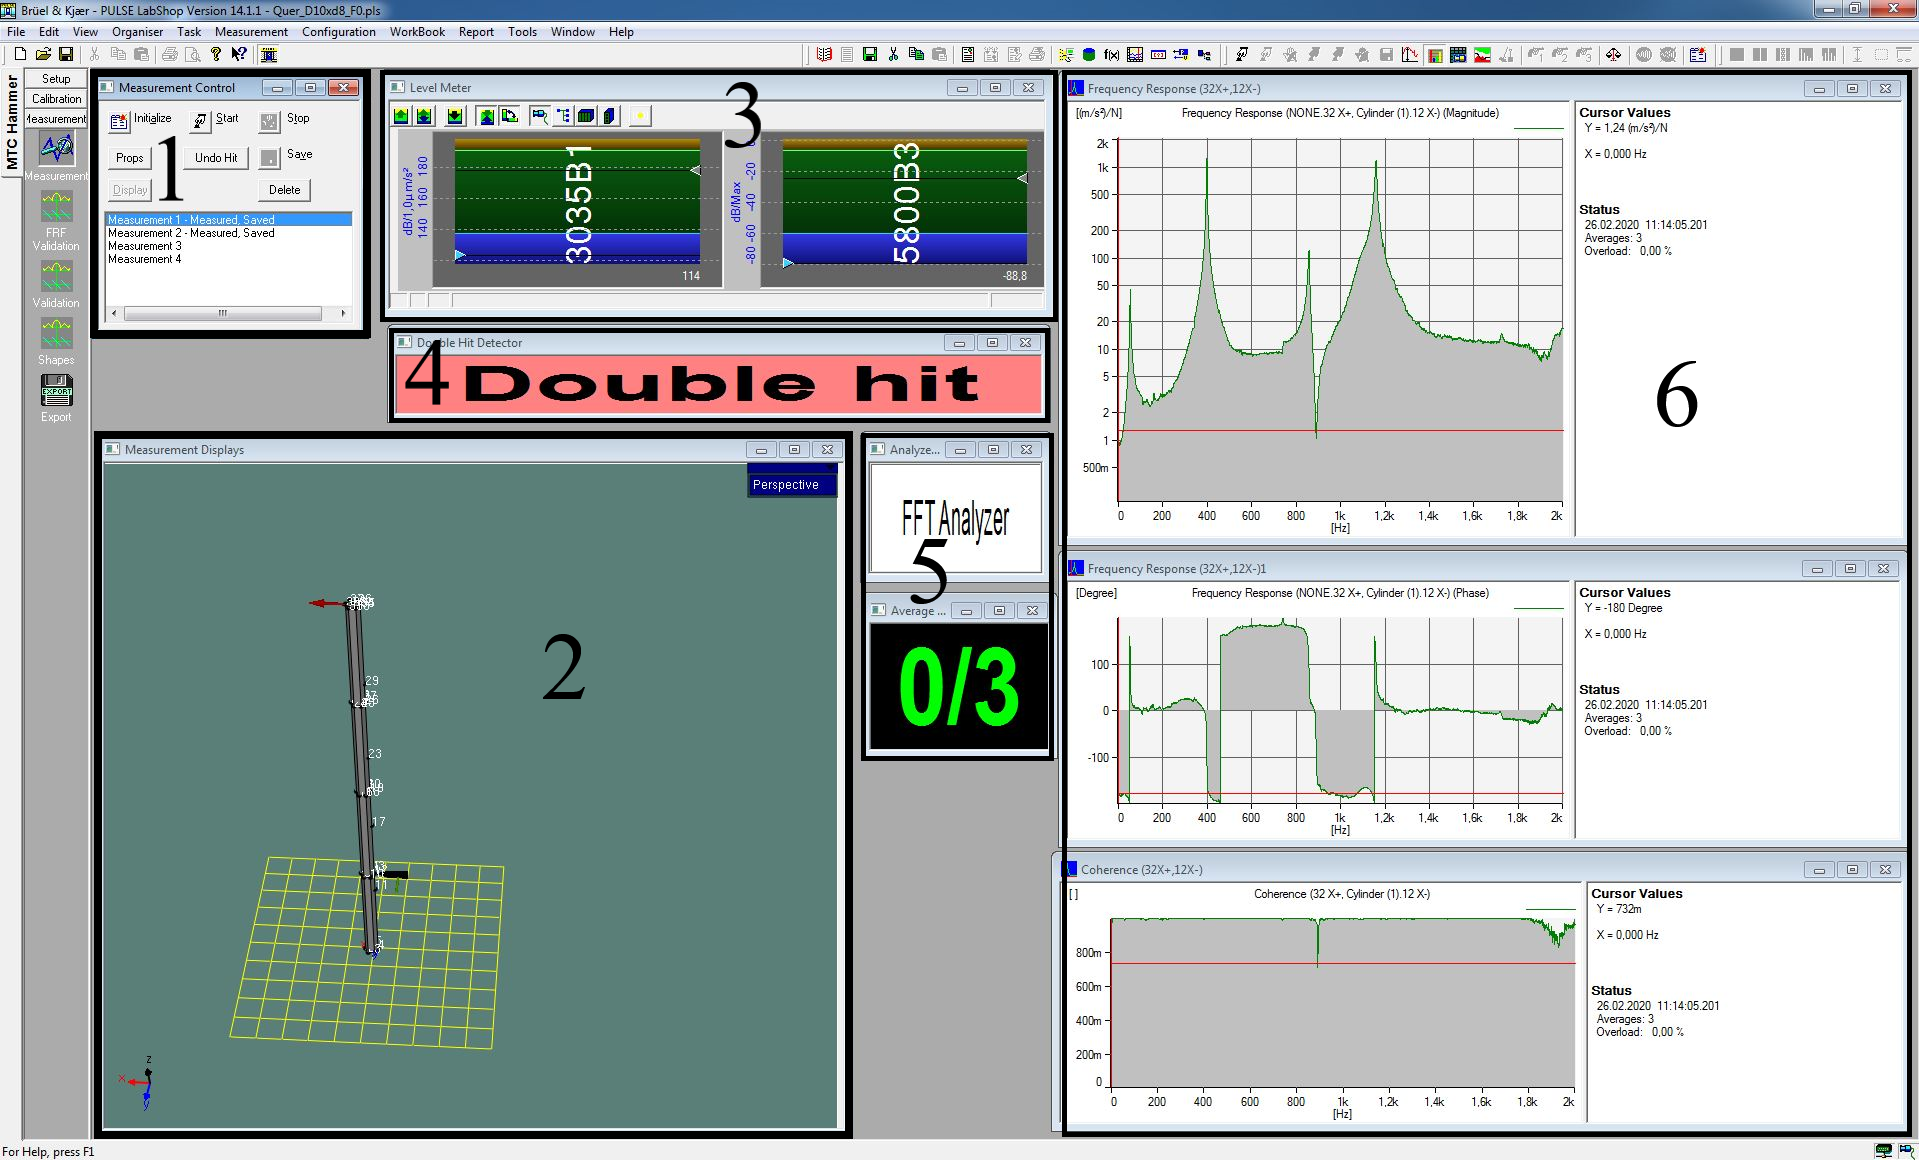
\includegraphics[width=0.96\linewidth, height=0.42\textheight]{Experimentelle_Untersuchungen/Schaft_10x8_0N_parallel_Messung.png}
		\caption{Userinterface für \textsc{PULSE LabShop} Version 14.1.1 von \textsc{Brüel \& Kj\ae{}r}.}
		\label{fig:B&K-Software}
	\end{figure}
	Die einzelnen Bildbereiche besitzen dabei folgende Bedeutung:
	\begin{itemize}
		\item Bereich 1: Steuerung der experimentelle Aktionen, einschließlich Initialisierung, Start, Stopp und Auswahl von Messpunkten. Für jeden Messpunkt werden die Ergebnissse von drei Messungen gemittelt.
		\item Bereich 2: Visualisierung eines dreidimensionales Modells der des Probenkörpers. Angezeigt werden die Punkte der Anregung (schwarzer Pfeil) und der Punkt der Beschleunigungsmessung (roter Pfeil).  und der Anzeige von Messpunkten.
		\item Bereich 3: Anzeige des aktuellen Messpegels für den Kraft und Beschleunigungssensor.
		\item Bereich 4: Mit diesem Erkennungsmodul werden eventuelle Doppelschläge angezeigt.
		\item Bereich 5: Anzeige der erfolgreich durchgeführten Messungen pro Messpunkt. 
		\item Bereich 6: Anzeige der gemessenen Übertragungsfunktion für den aktuellen Messpunkt (oben), Phasenwinkel (mitte) und Kohörenzfunktion (unten).
	\end{itemize}
	
	Es werden die Übertragungsfunktionen für vier Messpunkte am Schaft ermittelt. Mit den drei Wiederholungen je Messpunkt ergeben sich 12 Messungen pro Schaft. Die Weiterverarbeitung der Übertragungsfunktionen erfolgt mit der zweiten Software \textsc{ME'scopeVES} von \textsc{Vibrant Technology Inc.} Damit können die Modalparameter und auch die Modeformen ermittelt werden. Abschließend zeigt Abbildung \ref{fig:ME'scopeVES-Software} das dazugehörige Userinterface.
	
	\begin{figure}[H]
		\centering
		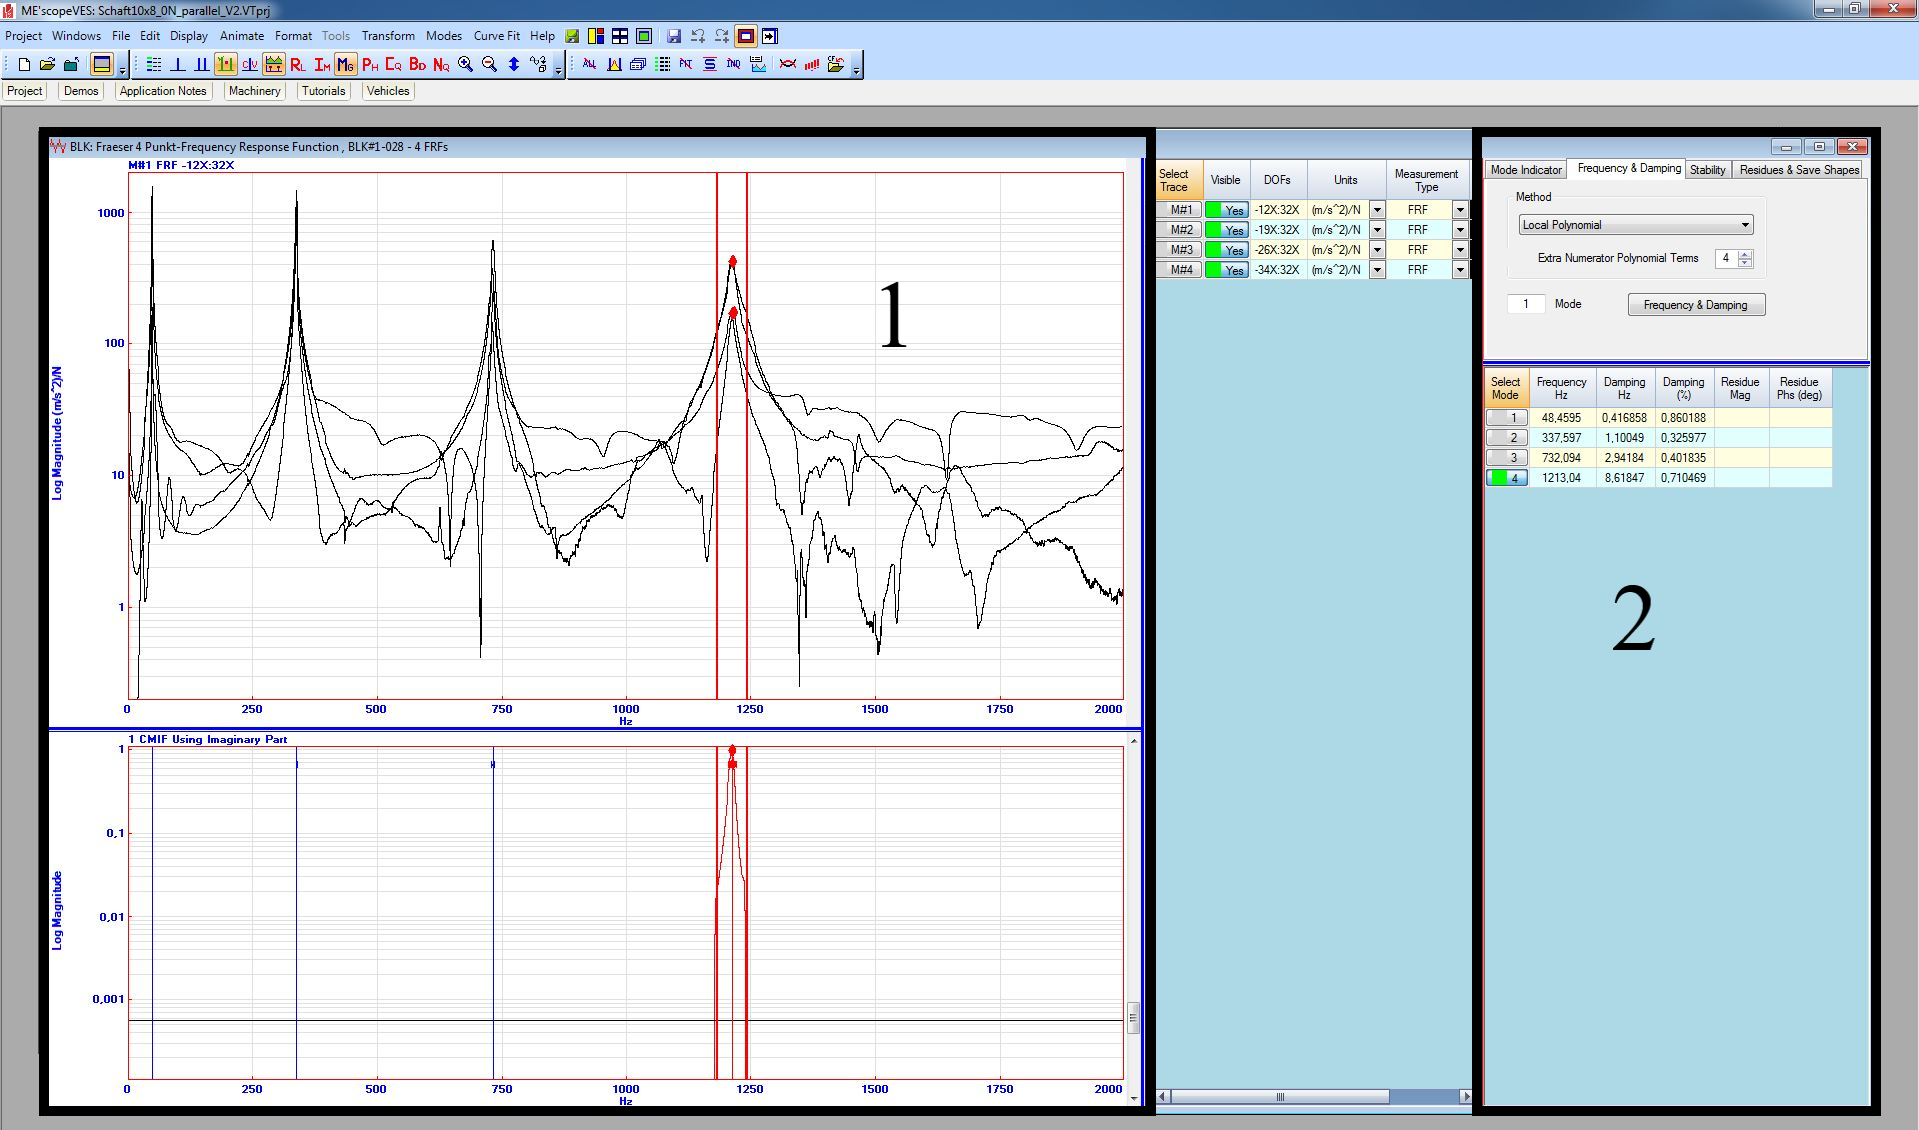
\includegraphics[width=0.97\linewidth, height=0.42\textheight]{Experimentelle_Untersuchungen/Schaft_10x8_0N_parallel_Ergebnisse.png}
		\caption{Userinterface der Software \textsc{ME'scopeVES} von \textsc{Vibrant Technology Inc.}}
		\label{fig:ME'scopeVES-Software}
	\end{figure}
	
	Der Bereich 1 zeigt die vier Übertragungsfunktionen in einem Diagramm. Gut zu erkennen sind die einzelnen Peaks, welche die Eigenfrequenzen darstellen. Im Bereich 2 sind die ermittelten Modalparameter (Frequenz und Dämpfung) für die ersten vier Biegemoden dargestellt.
	
	
	
	\subsection{Experimentelle Modalanalyse}\label{sec:Experimentelle Modalanalyse}
	Wie im Versuchsplan angegeben ist zuerst die experimentelle Identifikation der Modalparameter der Struktur durchzuführen. Die Eigenfrequenzen des Probekörper werden als wichtiger Kennwert durch die experimentelle Modalanalyse bestimmt.\\	
	
	Die Messung der Eigenfrequenz erfolgt nach der sogenannten Impulshammermethode. Der einseitige eingespannte HSC-Schaft wird hierfür an vier Punkten nacheinander angeregt. Beim Anschlagen mit dem Impulshammer (Typ 5800B3 von \textsc{Dytran Instruments}) wird das entstehende Kraftsignal aufgezeichnet. Zeitgleich erfolgt die Messung der Antwort mittels des Beschleunigungssensors (Typ 3035B3 von \textsc{Dytran Instruments}), welcher magnetisch mit dem Versuchskörper verbunden ist.\\
	
	Die vom Beschleunigungsmesser und Impulshammer erhaltenen Signale werden von Messsoftware \textsc{PULSE LabShop} verarbeitet und durch die Übertragungsfunktion dargestellt \cite{dossing1989strukturen}. Durch das Exportieren der Messergebnisse in die Software Modalanalyse-Software \textsc{ME'scopeVES} könne die Modalparameter berechnet werden. Im nächsten Kapitel werden die simulierten Eigenfrequenzen und die experimentellen Ergebnisse ausführlich analysiert und verglichen.
	
	

%% empty page %%%%%%%%%%%%%%%%%%%%%%%%%%%%%%%%%%%%%%%%%%
		%% empty page %%%%%%%%%%%%%%%%%%%%%%%%%%%%%%%%%%%%%%%%%%
	\newpage
	\pagestyle{empty}
	\ \\
	\newpage
	%%%%%%%%%%%%%%%%%%%%%%%%%%%%%%%%%%%%%%%%%%%%%%%%%%%%%%%%%
%%%%%%%%%%%%%%%%%%%%%%%%%%%%%%%%%%%%%%%%%%%%%%%%%%%%%%%%%%%%%%%%%%%%%%%%%%%%%%%%%%%%%%%%%%%%%%%%%%%%%%%%%%%%%%%%%%

		\pagestyle{fancy}
	\section{Ergebnisse} \label{sec:Ergebnisse}
	\subsection{Probe Nr. 1 (Schaft 10$\times$8)}
	Für die Simulationen wird das im Kapitel \ref{sec:Berechnungsmodell} beschriebene Modell verwendet. Die experimentellen Ergebnisse wurden mit dem in Kapitel  \ref{sec:Experimentelle Untersuchungen} beschriebenen Aufbau ermittelt. Die Versuchsschäfte sind aus Stahl und besitzen folgende Materialdaten: $\rho = 7800 \,\text{kg}/\text{m}^{3} $, $ E=2,1\cdot 10^{11} \,\text{N}/\text{m}^{2} $ und $ \nu=0,28 $. In den Abbildungen \ref{fig:Result-Schaft-10x8-Simulation-1-Mode} und \ref{fig:Result-Schaft-10x8-Simulation-2-Mode} ist die Abhängigkeit der Eigenfrequenzen von der Winkelgeschwindigkeit für $ e=0 $ dargestellt. In den Abbildungen \ref{fig:Result-Schaft-10x8-Simulation-1-Mode-ruhend} und \ref{fig:Result-Schaft-10x8-Simulation-2-Mode-ruhend} werden die Ergebnisse im ruhenden Inertialsystem angegeben, d.h. Drehzahl $ [1/s] $ des Schaftes zum steigenden Ast subtrahieren und zum fallenden Ast addieren.\\
	
	Wie allen Abbildungen zeigen, splitten sich die Eigenfrequenzen auf. Der steigende Ast wird als rückwärtiger Mode und der fallende Ast als vorwärtiger bezeichnet. Beide Äste fallen oder steigen linear. Eine Abhängigkeit der Eigenfrequenzen vom Exzentrizitätsfehler $ e $ konnte bei den Simulationen nicht festgestellt werden.\\
	
	Abbildung \ref{fig:Result-Schaft-10x8-Simulation-Durchbiegung} zeigt die Durchbiegung des Schaftes in Abhängigkeit der Winkelgeschwindigkeit $ \Omega $ bei einem festen Exzentrizitätsfehler $ e=0,001\,\text{m}$. Es ist ersichtlich, dass mit steigender Winkelgeschwindigkeit die Durchbiegung zunimmt. Der Zusammenhang zwischen Durchbiegung und $\Omega$ ist dabei quadratisch.\\
	
	Abbildung \ref{fig:Result-Schaft-10x8-Simulation-Zugkraft} zeigt die niedrigste Biegeeigenfrequenz abhängig von der Winkelgeschwindigkeit $ \Omega $ und der Zugkraft $ Fx $, die am Ende des Schaftes wirkt. Für den Exzentrizitätsfehler gilt erneut $ e=0 $. Es lässt sich beobachten, dass die Eigenfrequenzen mit steigender Zugkraft zunehmen. Grund hierfür ist der Spannungsversteifende Einfluss der Zugkraft.
	
	\begin{figure}[H]
		\centering
		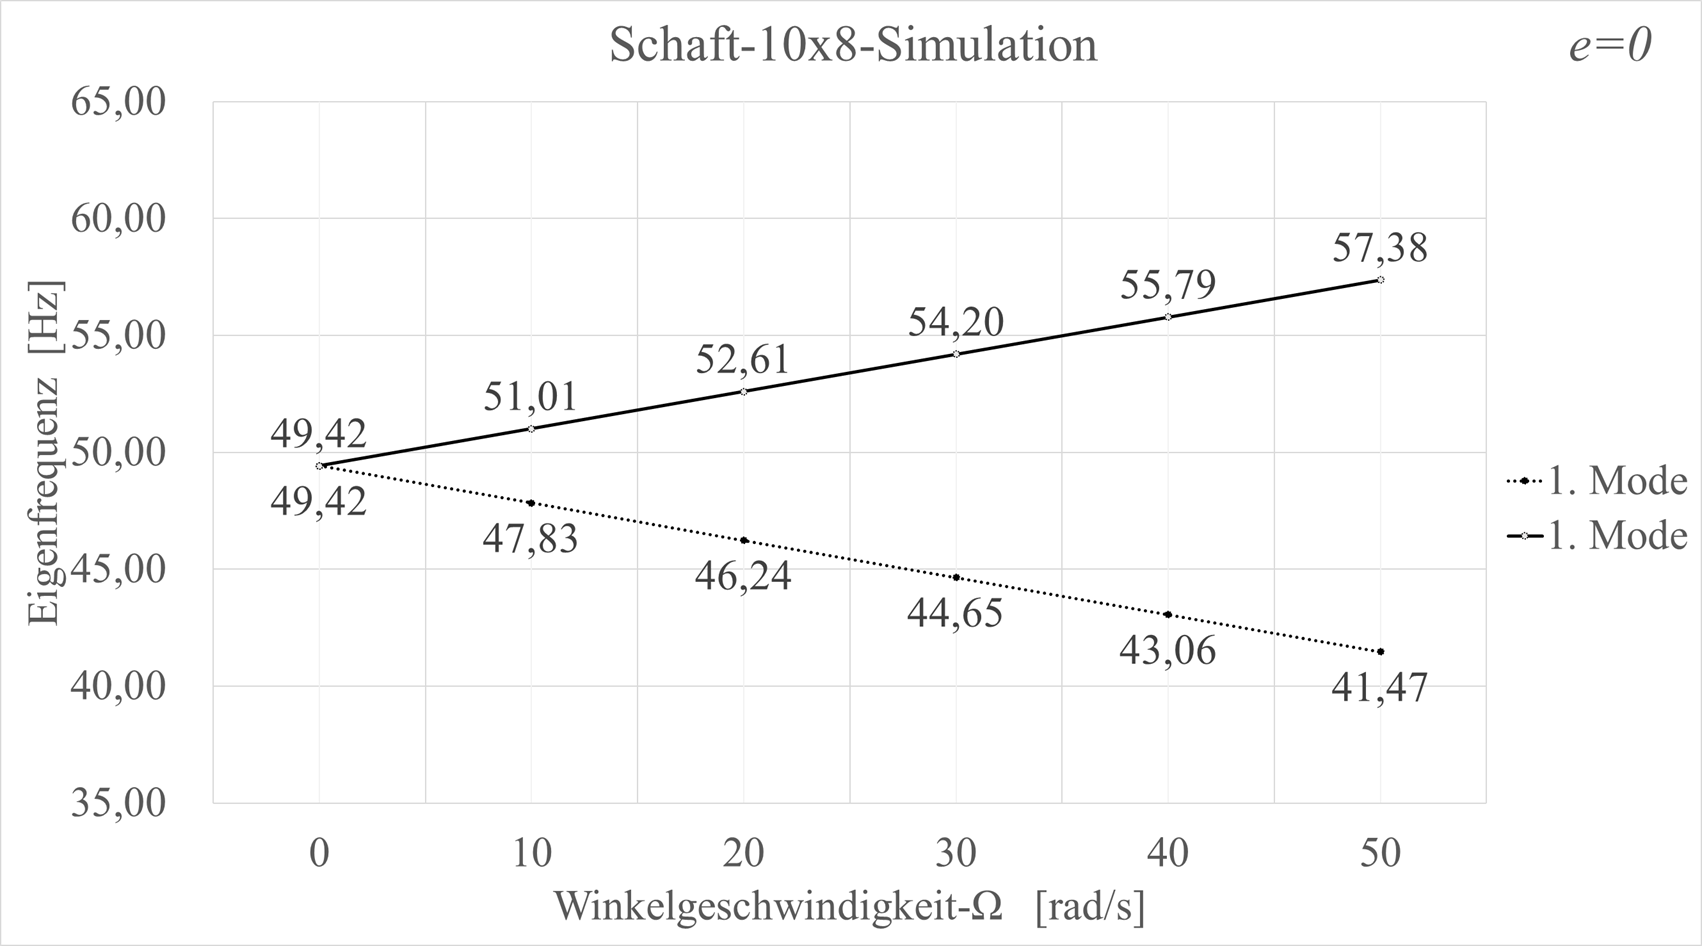
\includegraphics[width=0.95\linewidth, height=0.35\textheight]{Ergebnisse/Schaft_10x8_1Mode_Simu}
		\caption{Eigenfrequenzen vom 1. Biegemode in Abhängigkeit der Winkelgeschwindigkeit bei einem Exzentrizitätsfehler von $ e=0 $. Berechnungsparameter: Schaft $ 10\times8 $, $\rho = 7800 \,\text{kg}/\text{m}^{3} $, $ E=2,1\cdot 10^{11} \,\text{N}/\text{m}^{2} $, $ \nu=0,28 $.}
		\label{fig:Result-Schaft-10x8-Simulation-1-Mode}
	\end{figure}

	\begin{figure}[H]
		\centering
		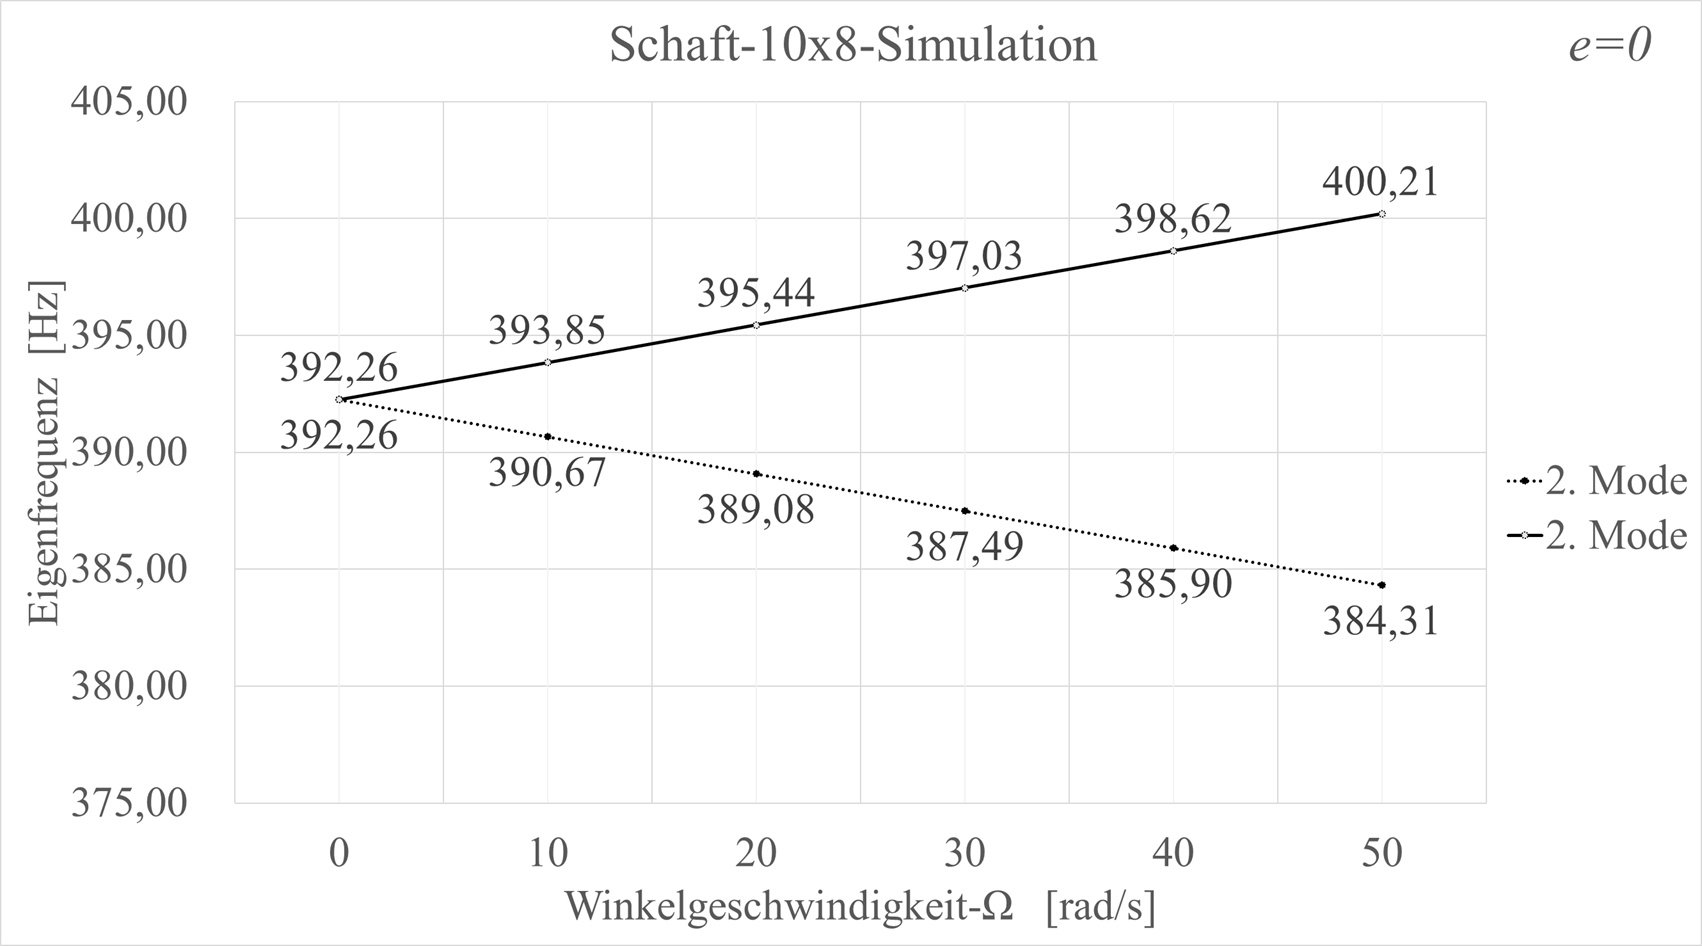
\includegraphics[width=0.95\linewidth, height=0.36\textheight]{Ergebnisse/Schaft_10x8_2Mode_Simu}
		\caption{Eigenfrequenzen vom 2. Biegemode in Abhängigkeit der Winkelgeschwindigkeit bei einem Exzentrizitätsfehler von $ e=0 $. Berechnungsparameter: Schaft $ 10\times8 $, $\rho = 7800 \,\text{kg}/\text{m}^{3} $, $ E=2,1\cdot 10^{11} \,\text{N}/\text{m}^{2} $, $ \nu=0,28 $.}
		\label{fig:Result-Schaft-10x8-Simulation-2-Mode}
	\end{figure}

	\begin{figure}[H]
		\centering
		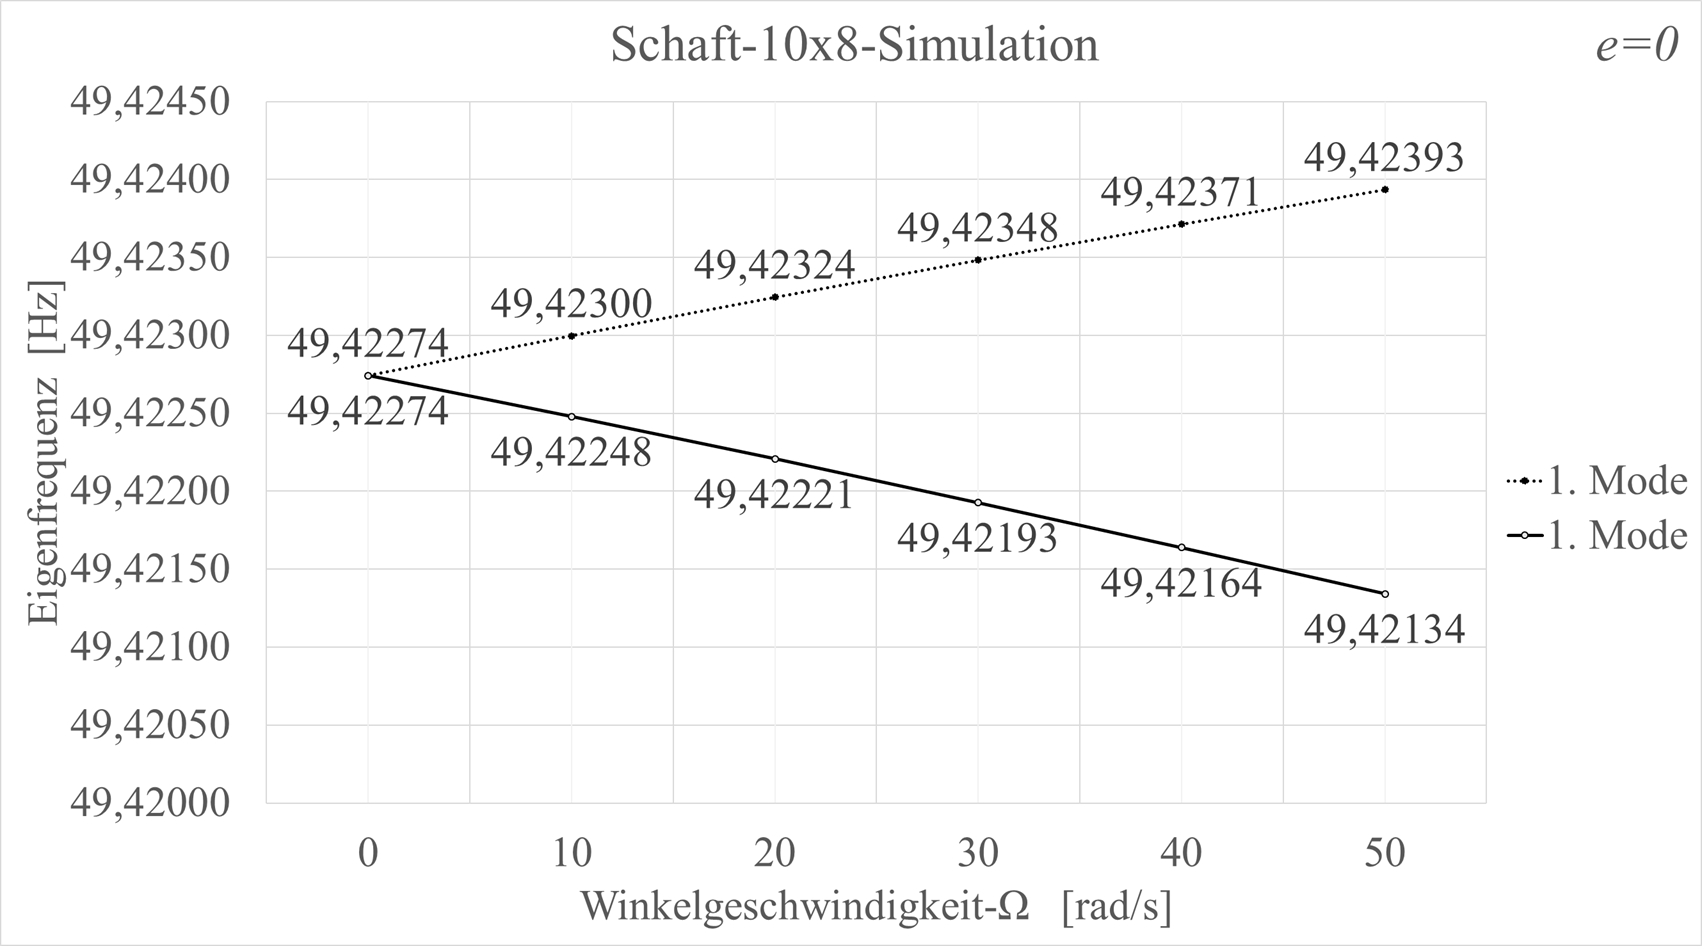
\includegraphics[width=0.95\linewidth, height=0.36\textheight]{Ergebnisse/Schaft_10x8_1Mode_Simu_ruhend}
		\caption{Eigenfrequenzen vom 1. Biegemode in Abhängigkeit der Winkelgeschwindigkeit bei einem Exzentrizitätsfehler von $ e=0 $ im ruhenden Inertialsystem. Berechnungsparameter: Schaft $ 10\times8 $, $\rho = 7800 \,\text{kg}/\text{m}^{3} $, $ E=2,1\cdot 10^{11} \,\text{N}/\text{m}^{2} $, $ \nu=0,28 $.}
		\label{fig:Result-Schaft-10x8-Simulation-1-Mode-ruhend}
	\end{figure}

	\begin{figure}[H]
		\centering
		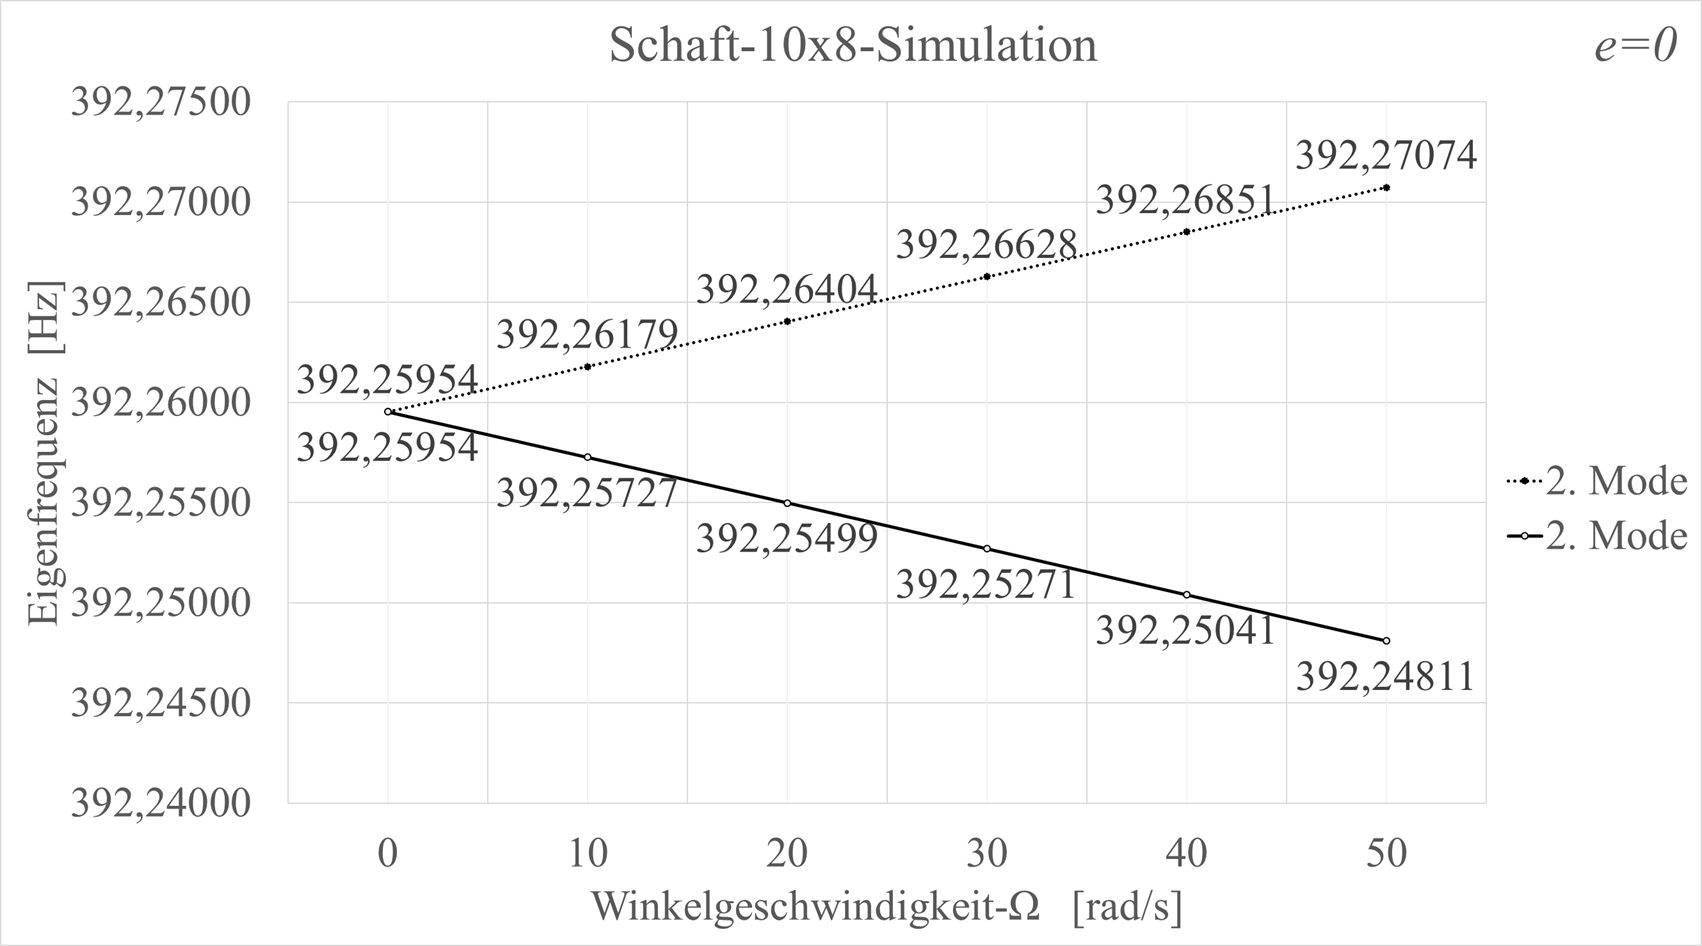
\includegraphics[width=0.95\linewidth, height=0.36\textheight]{Ergebnisse/Schaft_10x8_2Mode_Simu_ruhend}
		\caption{Eigenfrequenzen vom 2. Biegemode in Abhängigkeit der Winkelgeschwindigkeit bei einem Exzentrizitätsfehler von $ e=0 $ im ruhenden Inertialsystem. Berechnungsparameter: Schaft $ 10\times8 $, $\rho = 7800 \,\text{kg}/\text{m}^{3} $, $ E=2,1\cdot 10^{11} \,\text{N}/\text{m}^{2} $, $ \nu=0,28 $.}
		\label{fig:Result-Schaft-10x8-Simulation-2-Mode-ruhend}
	\end{figure}
	
	\begin{figure}[H]
		\centering
		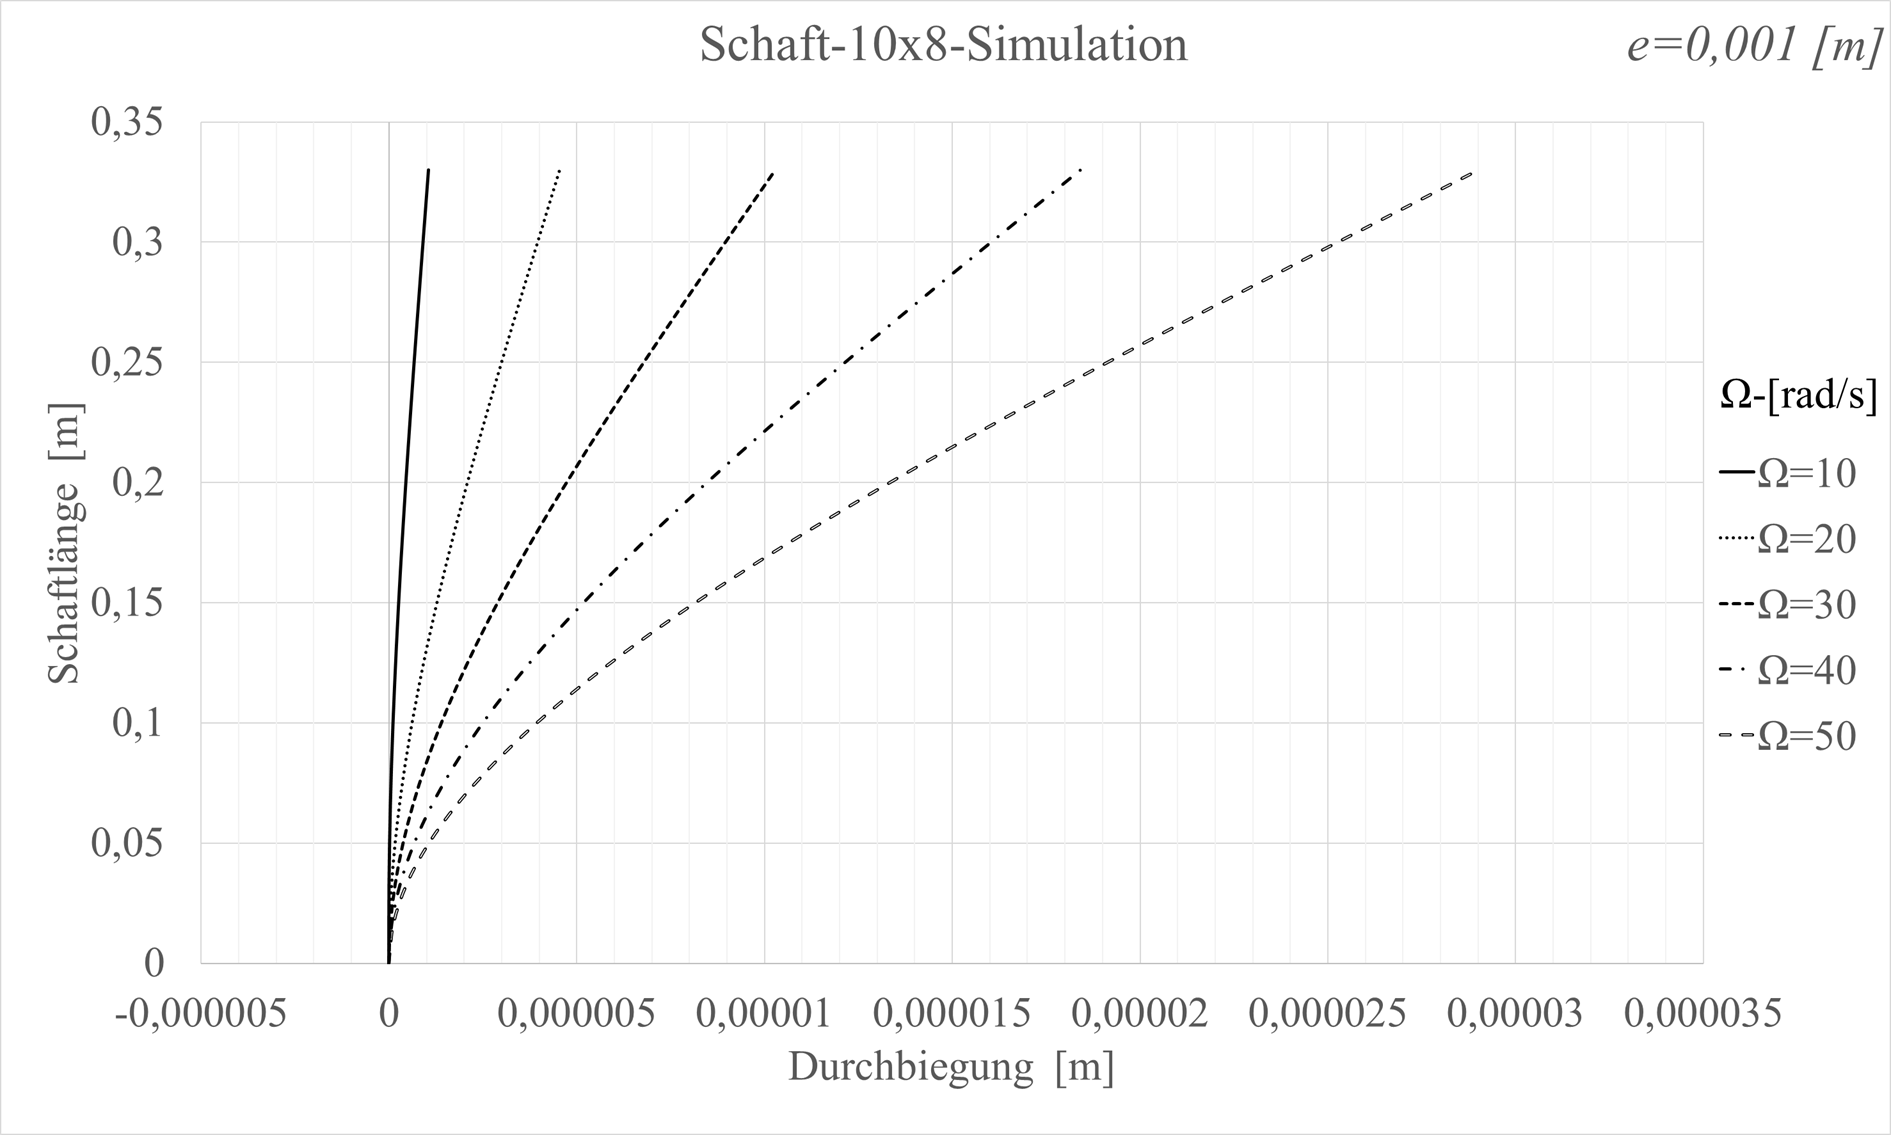
\includegraphics[width=0.95\linewidth, height=0.40\textheight]{Ergebnisse/Schaft_10x8_Biegung_Simu} 
		\caption{Durchbiegung in Abhängigkeit der Winkelgeschwindigkeit bei einem Exzentrizitätsfehler von $ e=0,001\,\text{m}$. Berechnungsparameter: Schaft $ 10\times8 $, $\rho = 7800 \,\text{kg}/\text{m}^{3} $, $ E=2,1\cdot 10^{11} \,\text{N}/\text{m}^{2} $, $ \nu=0,28 $.}
		\label{fig:Result-Schaft-10x8-Simulation-Durchbiegung}
	\end{figure}

	
	\begin{figure}[H]
		\centering
		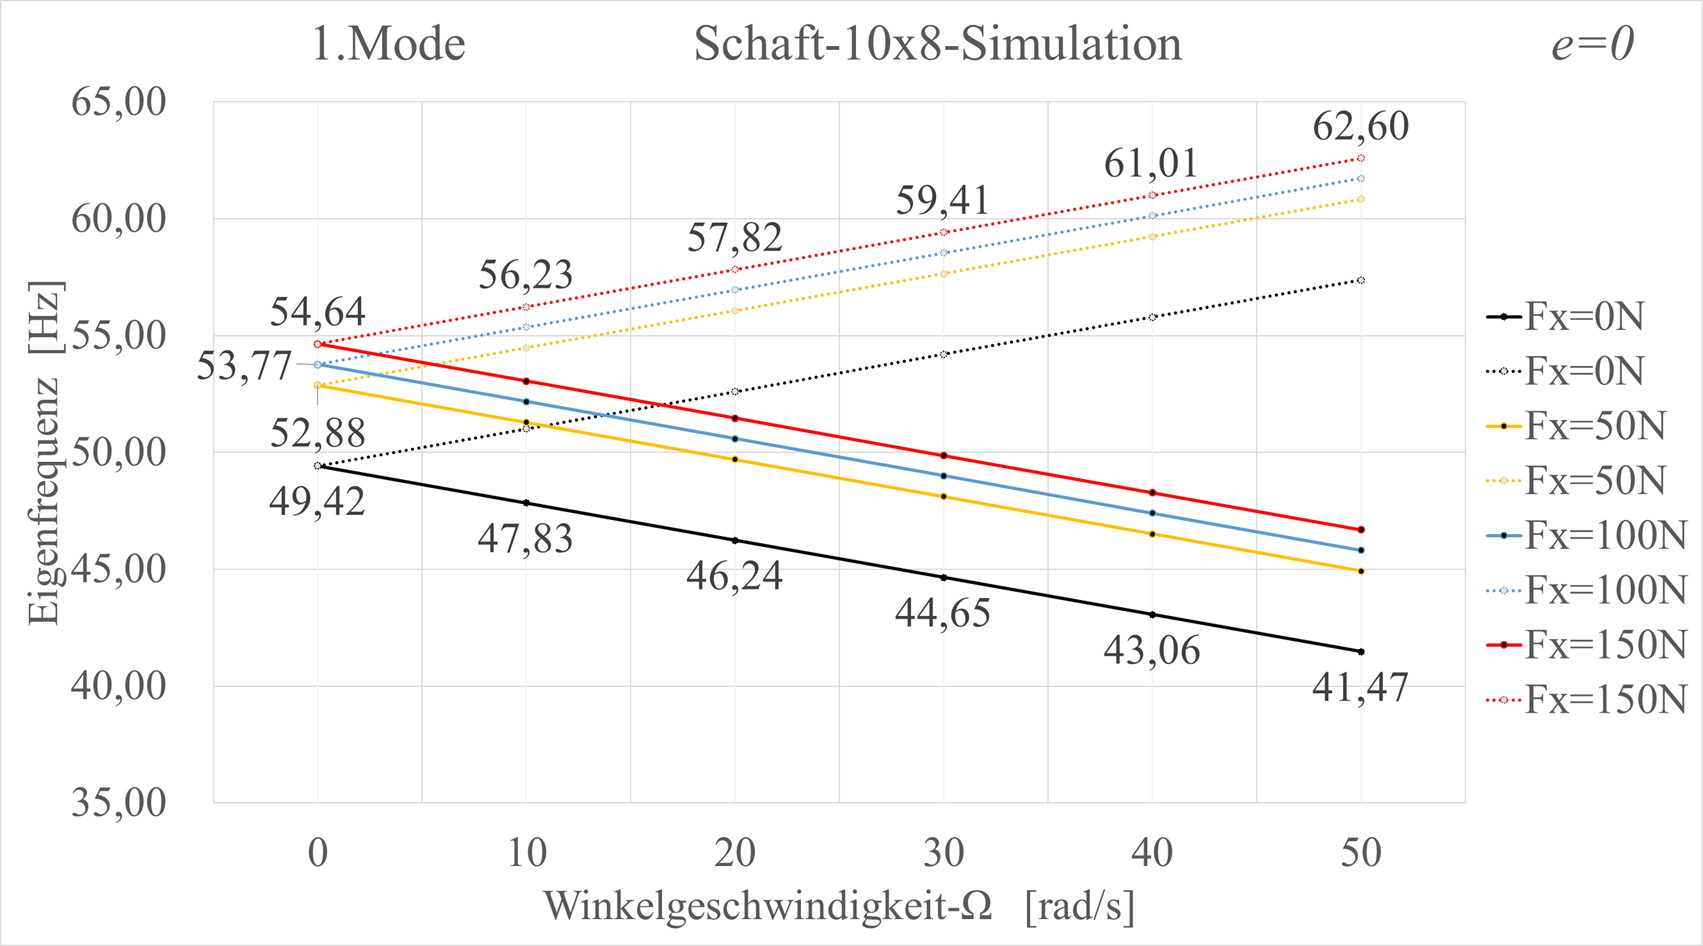
\includegraphics[width=0.93\linewidth, height=0.33\textheight]{Ergebnisse/Schaft_10x8_Zugkraft_Simu} 
		\caption{Eigenfrequenzen vom 1. Biegemode in Abhängigkeit der Winkelgeschwindigkeit $ \Omega $ und der Zugkraft $ Fx $ bei bei einem Exzentrizitätsfehler von $ e=0 $. Berechnungsparameter: Schaft $ 10\times8 $, $\rho = 7800 \,\text{kg}/\text{m}^{3} $, $ E=2,1\cdot 10^{11} \,\text{N}/\text{m}^{2} $, $ \nu=0,28 $.}
		\label{fig:Result-Schaft-10x8-Simulation-Zugkraft}
	\end{figure}
	
	Die experimentellen Ergebnissen werden gemäß den verschiedenen Messrichtungen des Beschleunigungssensors in die zwei Fälle unterteilt. Die Messrichtung erfolgt entweder parallel oder senkrecht zur Anregungsrichtung. Nach Gleichung \ref{equ:Verhältnis-Rotaion-und-Radialkraft} kann die Radialkraft in ein Produkt aus Exzentrizitätsfehler ($ e=0,001\,\text{m}$) und Winkelgeschwindigkeit umgerechnet werden. Weitere experimentelle Ergebnisse sind in den Abbildungen \ref{fig:Result-Schaft-10x8-1Mode-Ver1} bis \ref{fig:Result-Schaft-10x8-2Mode-Ver3} dargestellt.
	
	\begin{figure}[H]
		\centering
		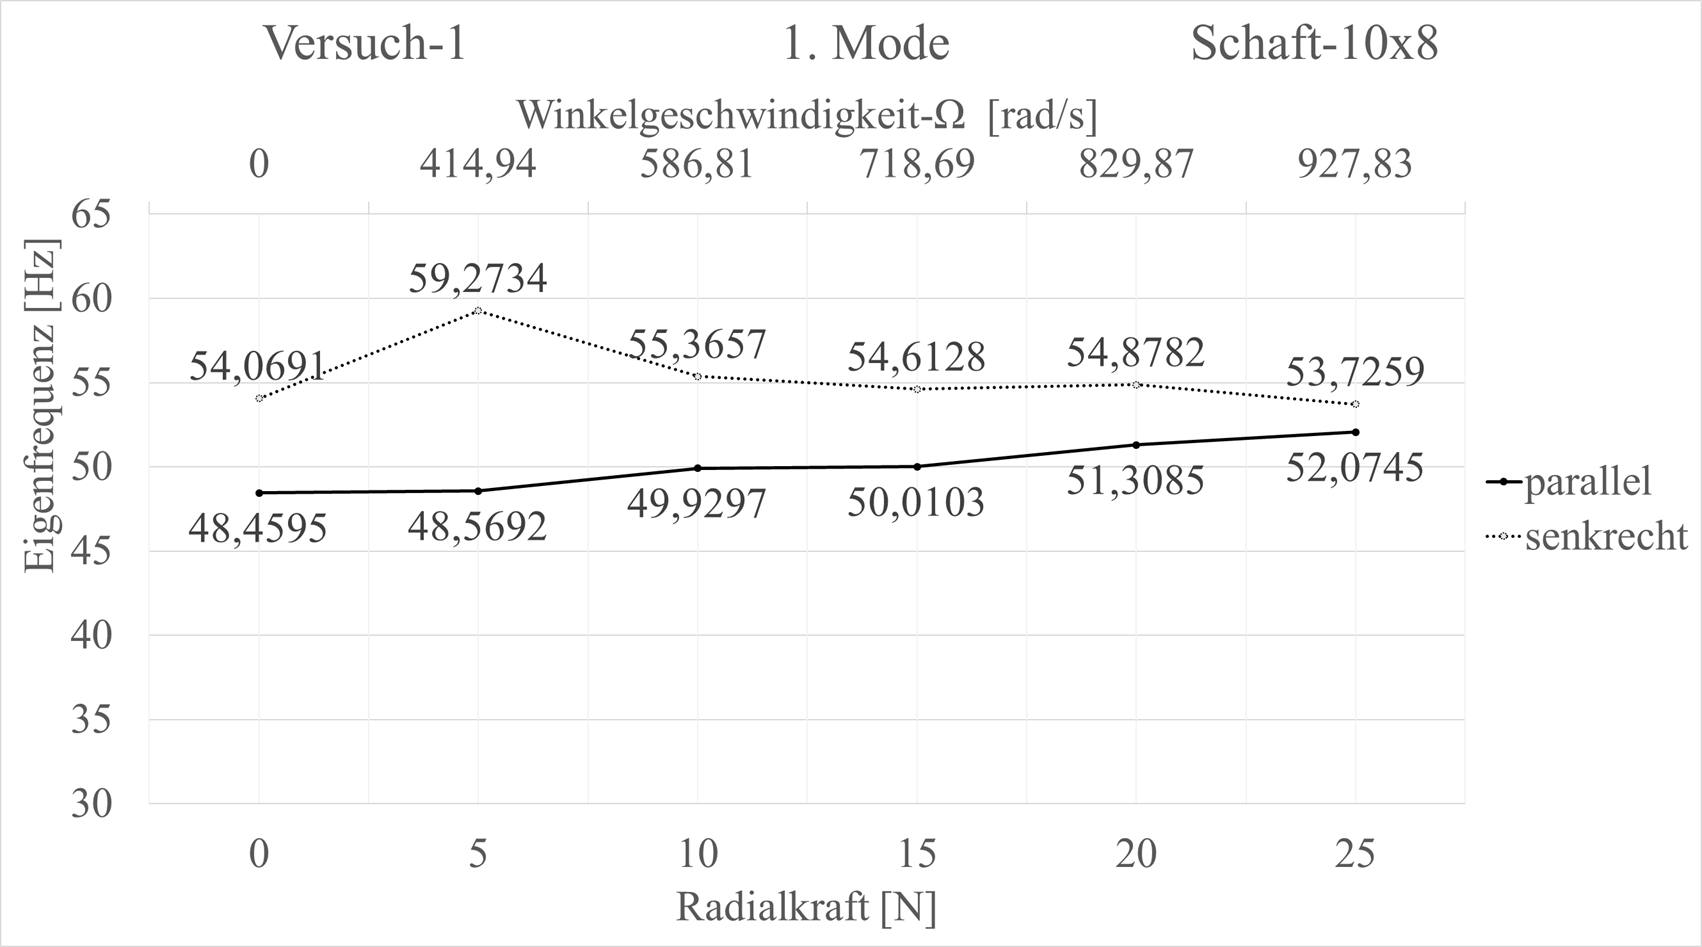
\includegraphics[width=0.93\linewidth, height=0.33\textheight]{Ergebnisse/Schaft_10x8_1Mode_ver1} 
		\caption{Gemessene Eigenfrequenzen vom 1. Biegemode in Abhängigkeit der Vorspannkraft. Angabe der Eigenfrequenzen parallel und senkrecht zur Vorspannrichtung. (Probe Nr. 1 (Schaft $ 10\times8 $ ), Versuchsreihe 1)}
		\label{fig:Result-Schaft-10x8-1Mode-Ver1}
	\end{figure}

	\begin{figure}[H]
		\centering
		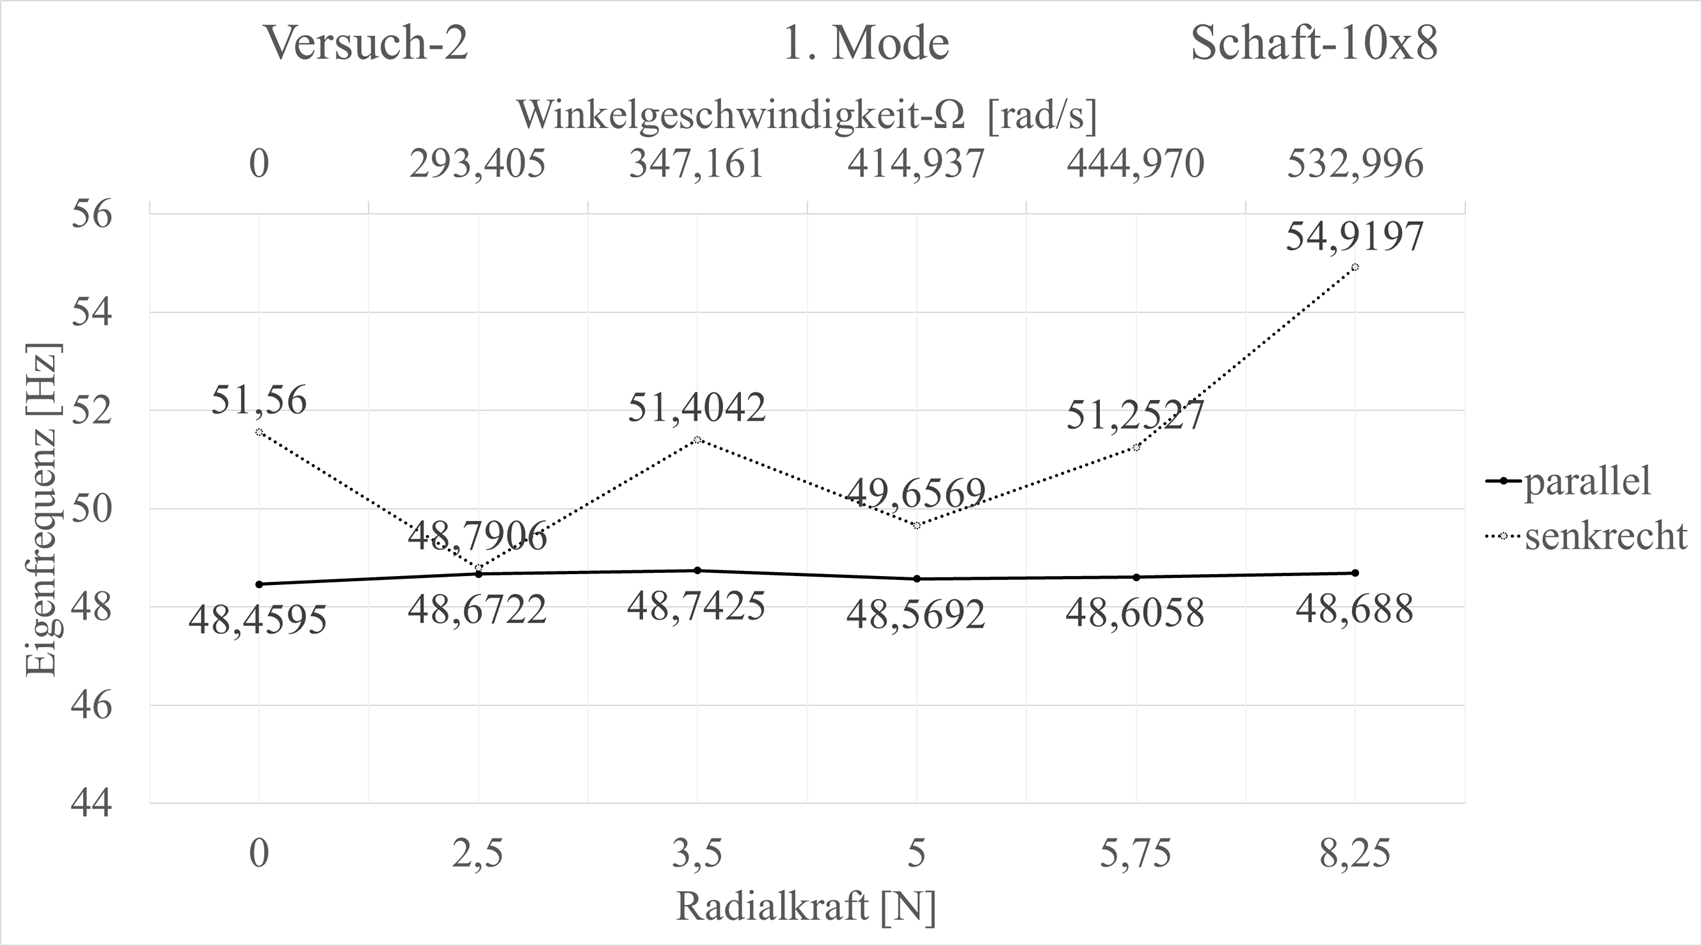
\includegraphics[width=0.95\linewidth, height=0.36\textheight]{Ergebnisse/Schaft_10x8_1Mode_ver2}
		\caption{Gemessene Eigenfrequenzen vom 1. Biegemode in Abhängigkeit der Vorspannkraft. Angabe der Eigenfrequenzen parallel und senkrecht zur Vorspannrichtung (Probe Nr. 1 (Schaft $ 10\times8 $ ), Versuchsreihe 2).}
		\label{fig:Result-Schaft-10x8-1Mode-Ver2}
	\end{figure}

	\begin{figure}[H]
		\centering
		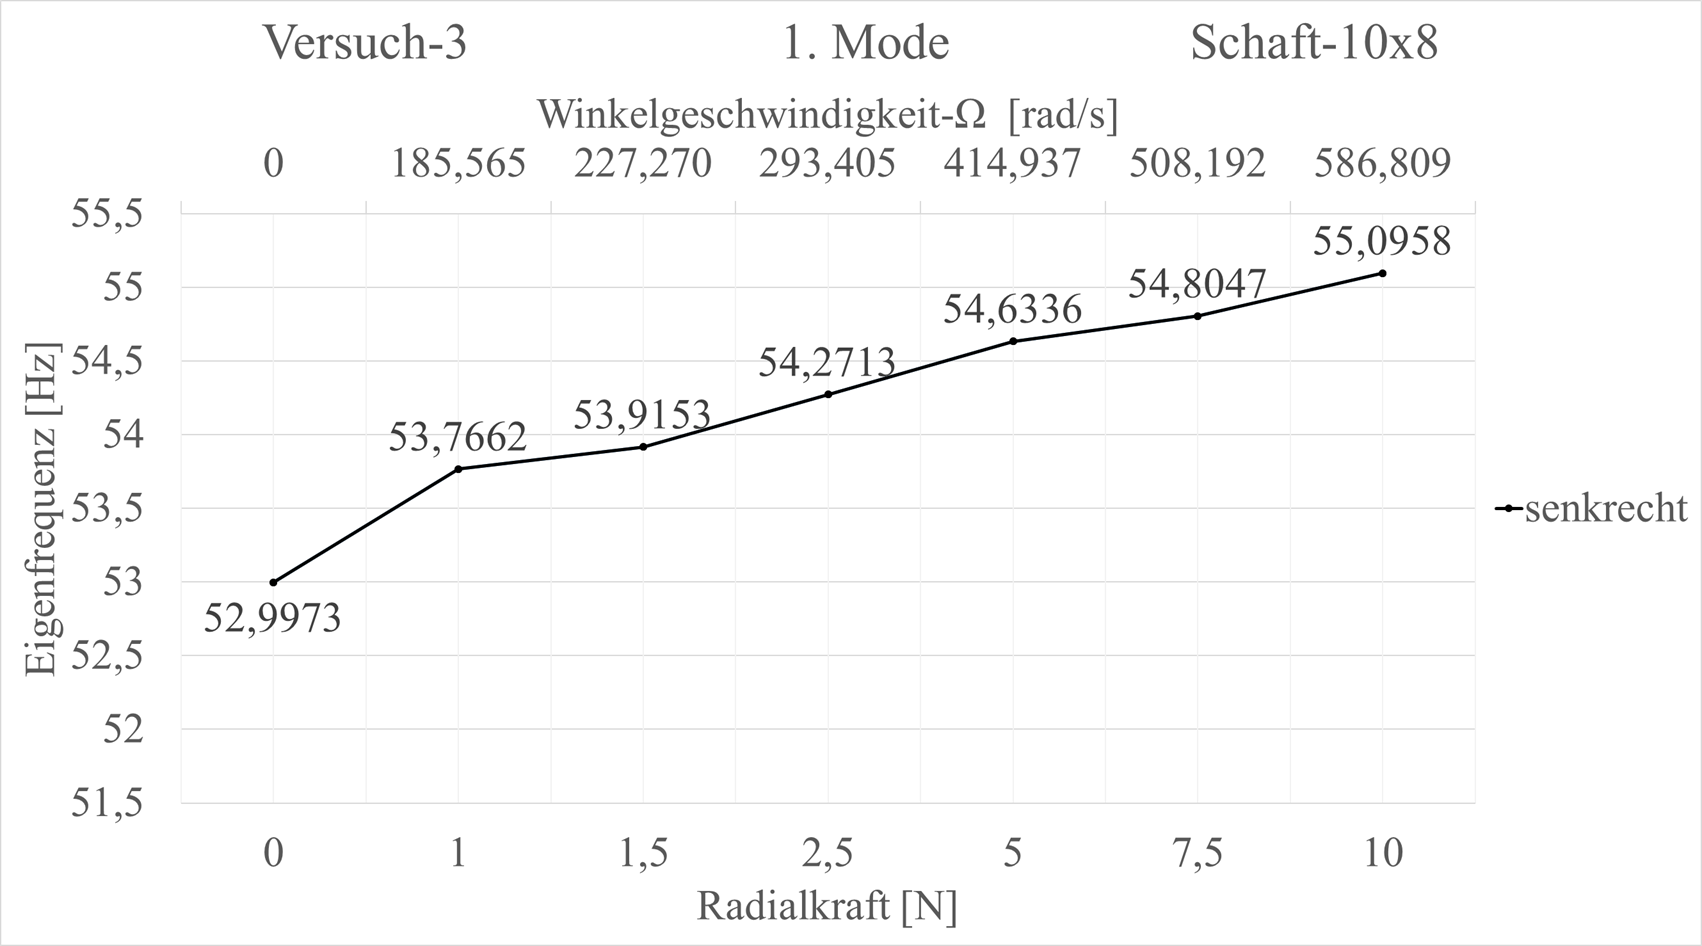
\includegraphics[width=0.95\linewidth, height=0.36\textheight]{Ergebnisse/Schaft_10x8_1Mode_ver3}
		\caption{Gemessene Eigenfrequenzen vom 1. Biegemode in Abhängigkeit der Vorspannkraft. Angabe der Eigenfrequenzen senkrecht zur Vorspannrichtung (Probe Nr. 1 (Schaft $ 10\times8 $), Versuchsreihe 3).}
		\label{fig:Result-Schaft-10x8-1Mode-Ver3}
	\end{figure}

	\begin{figure}[H]
		\centering
		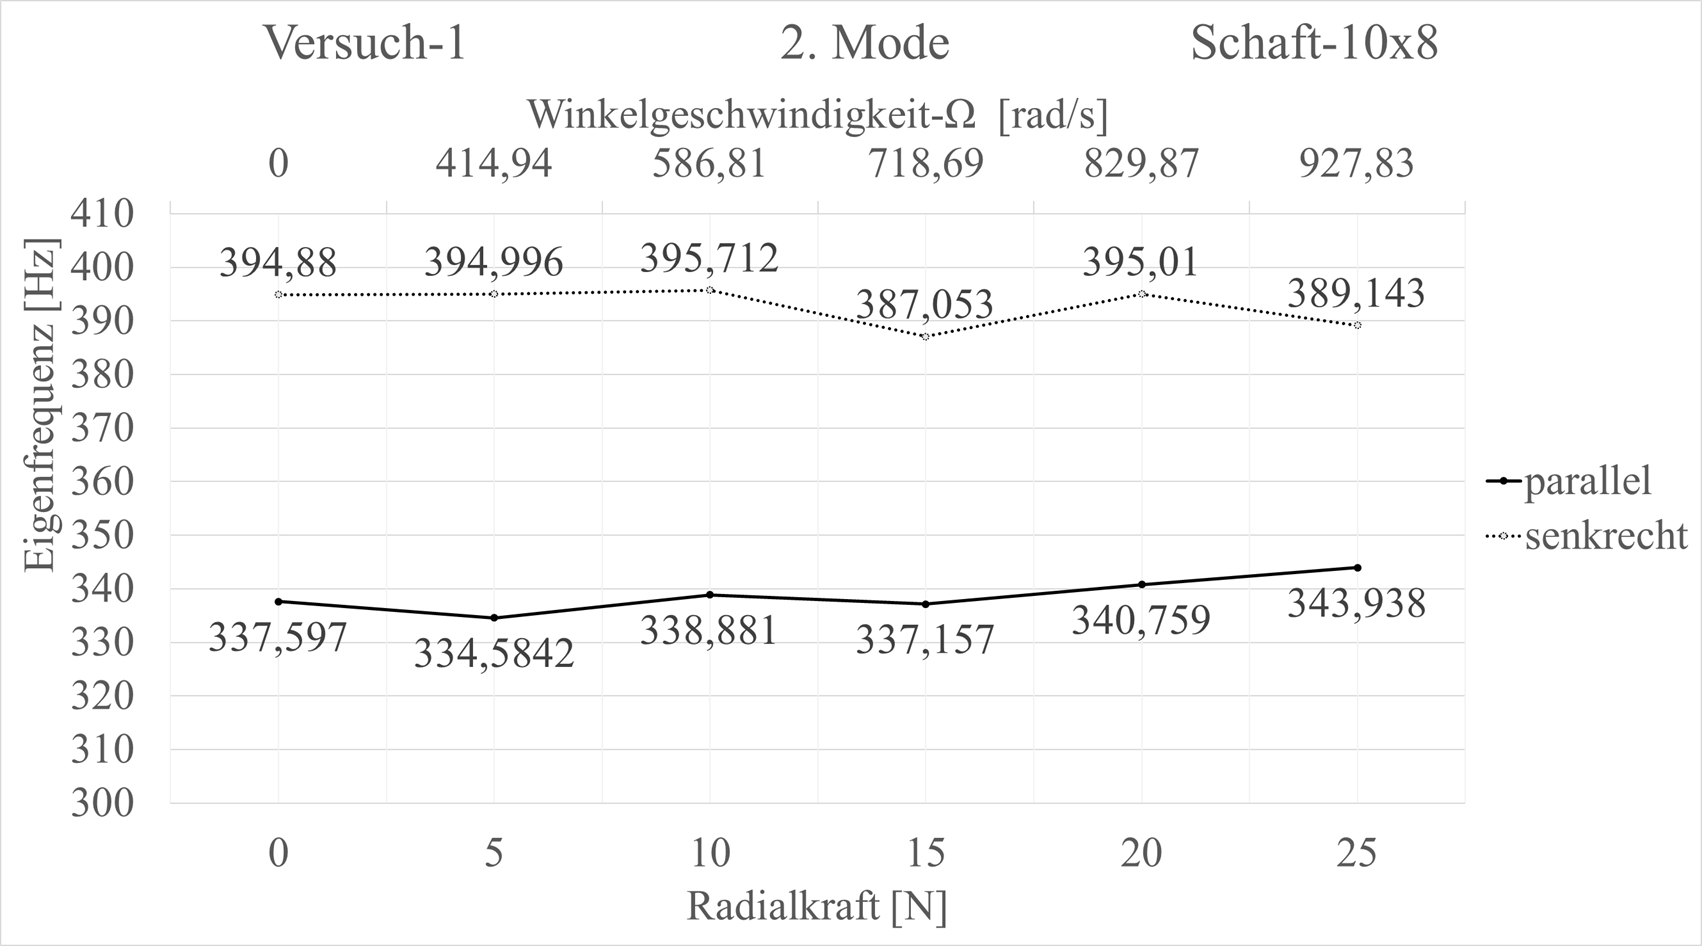
\includegraphics[width=0.95\linewidth, height=0.36\textheight]{Ergebnisse/Schaft_10x8_2Mode_ver1} 
		\caption{Gemessene Eigenfrequenzen vom 2. Biegemode in Abhängigkeit der Vorspannkraft. Angabe der Eigenfrequenzen parallel und senkrecht zur Vorspannrichtung (Probe Nr. 1 (Schaft $ 10\times8 $ ), Versuchsreihe 1).}
		\label{fig:Result-Schaft-10x8-2Mode-Ver1}
	\end{figure}

	\begin{figure}[H]
		\centering
		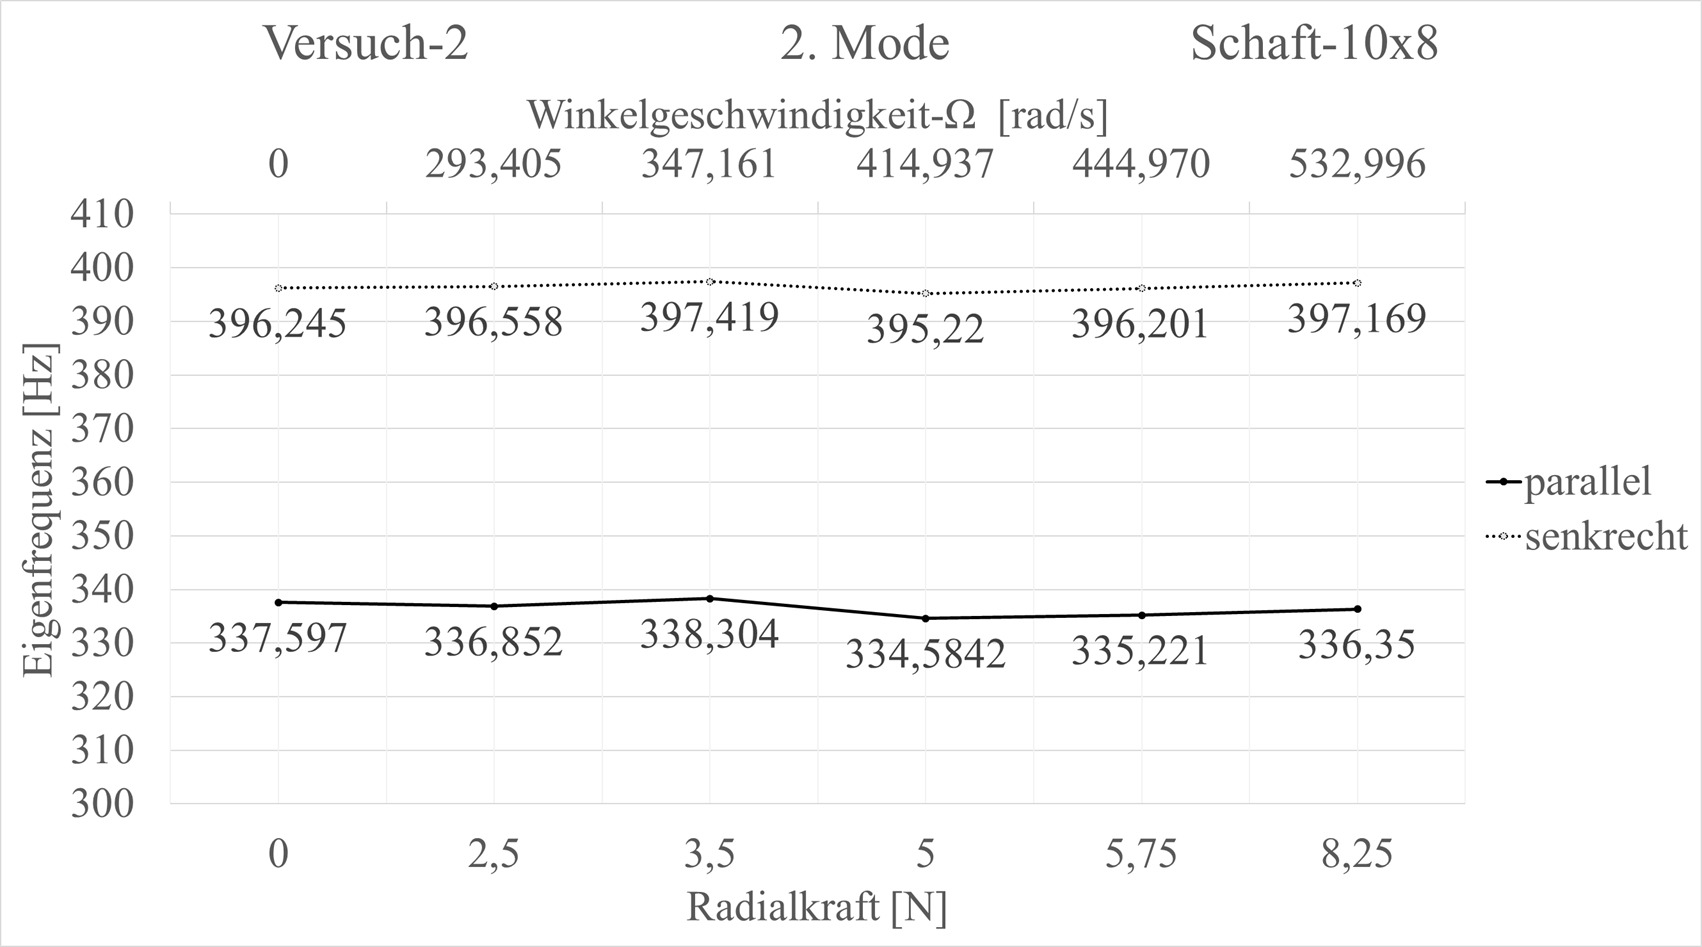
\includegraphics[width=0.95\linewidth, height=0.36\textheight]{Ergebnisse/Schaft_10x8_2Mode_ver2}
		\caption{Gemessene Eigenfrequenzen vom 1. Biegemode in Abhängigkeit der Vorspannkraft. Angabe der Eigenfrequenzen parallel und senkrecht zur Vorspannrichtung (Probe Nr. 1 (Schaft $ 10\times8 $ ), Versuchsreihe 2).}
		\label{fig:Result-Schaft-10x8-2Mode-Ver2}
	\end{figure}

	\begin{figure}[H]
		\centering
		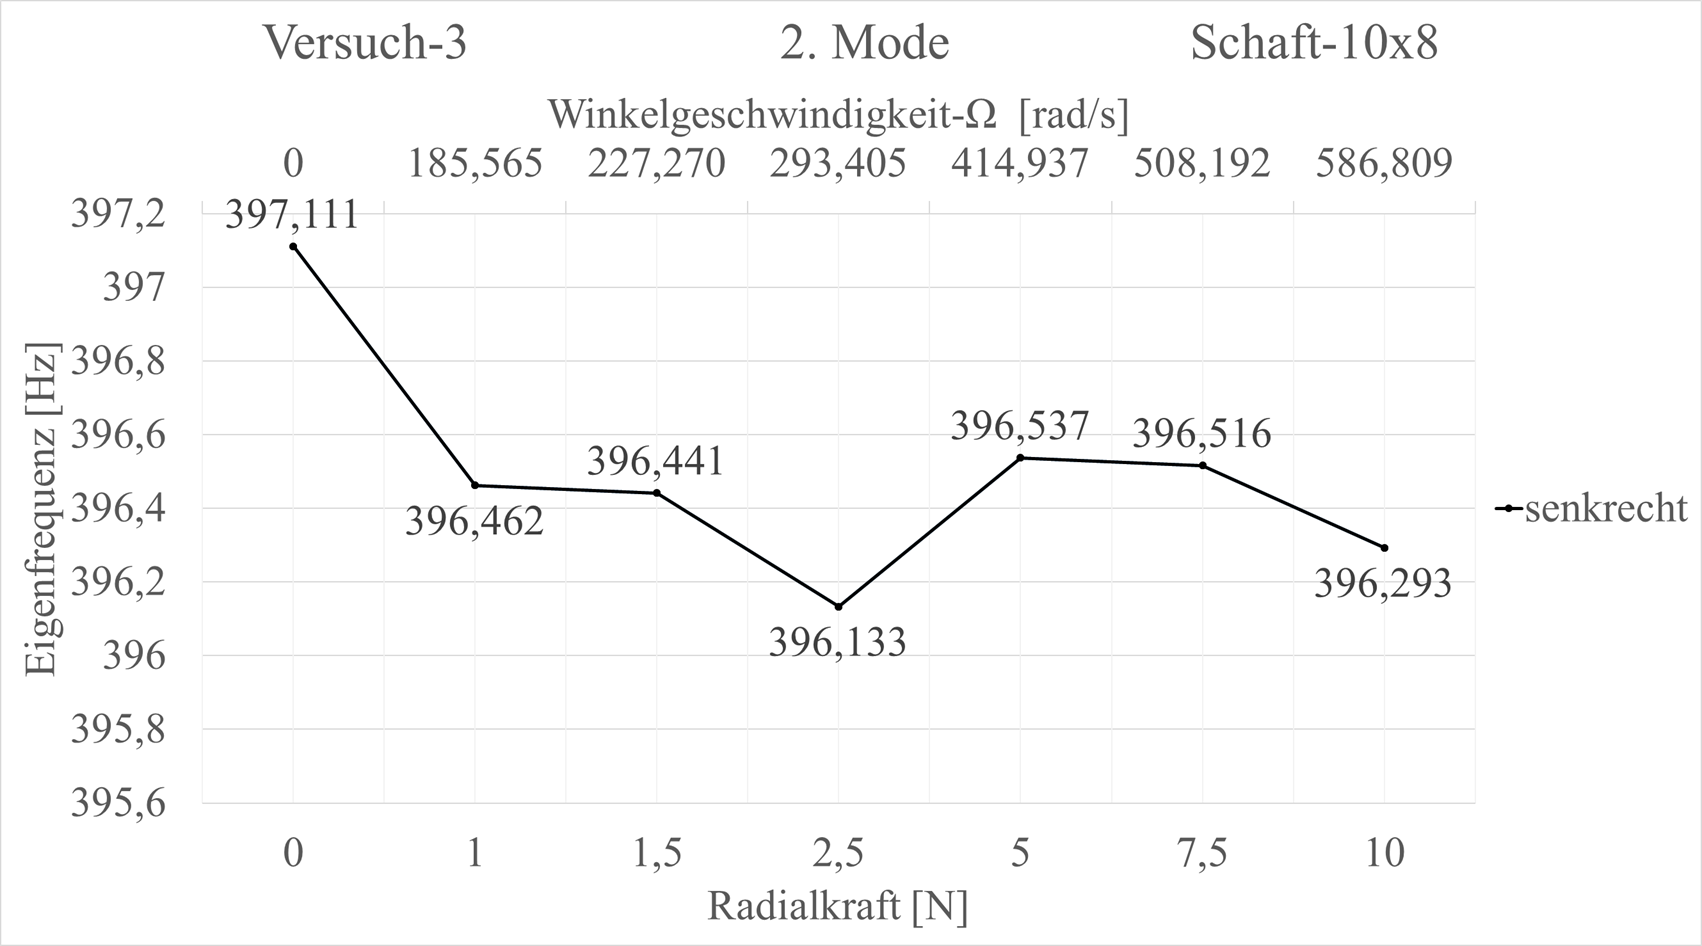
\includegraphics[width=0.95\linewidth, height=0.36\textheight]{Ergebnisse/Schaft_10x8_2Mode_ver3}
		\caption{Gemessene Eigenfrequenzen vom 1. Biegemode in Abhängigkeit der Vorspannkraft. Angabe der Eigenfrequenzen senkrecht zur Vorspannrichtung (Probe Nr. 1 (Schaft $ 10\times8 $), Versuchsreihe 3).}
		\label{fig:Result-Schaft-10x8-2Mode-Ver3}
	\end{figure}
	
	Die Abbildungen \ref{fig:Result-Schaft-10x8-1Mode-Ver1} bis \ref{fig:Result-Schaft-10x8-1Mode-Ver3} zeigen die Ergebnisse für die ersten beiden Moden. Eine klare Abhängigkeit der Eigenfrequenzen lässt sich nur schwer ableiten. Tendenziell nehmen die Eigenfrequenzen senkrecht zur Vorspannrichtung mit zunehmender Vorspannkraft leicht zu (vgl. Abbildung \ref{fig:Result-Schaft-10x8-1Mode-Ver2} und \ref{fig:Result-Schaft-10x8-1Mode-Ver3}). Parallel zur Vorspannrichtung ist der Einfluss der Vorspannkraft auf die Eigenfrequenzen geringer. Die Ungenauigkeiten der experimentellen Ergebnisse begründen sich mit verschiedenen Störungen und Messungenauigkeiten. Die Eigenfrequenz des ersten Modes im senkrechten Fall zeigt, dass mit zunehmender Radialkraft die Eigenfrequenz allmählich zunimmt. Werden die gemessenen und berechneten Eigenfrequenzen für den ruhenden Schaft verglichen, so fällt auf, dass die gemessenen Werte niedriger sind. Ursache dafür sind die zusätzliche Massen durch den Beschleunigungssensor und die Feder. 
	
	
	\subsection{Probe Nr. 2 (Schaft 10$\times$9)}	
	Als zweiter Probekörper wird der Schaft-$10\times9 $ betrachtet. Die Materialparameter sind identisch zu Probe Nr.1. In den Abbildungen \ref{fig:Result-Schaft-10x9-Simulation-1-Mode} bis \ref{fig:Result-Schaft-10x9-Simulation-Zugkraft} sind zunächst wieder die Simulationsergebnisse dargestellt. Die experimentellen Ergebnisse sind anschließend in den Abbildungen \ref{fig:Result-Schaft-10x9-1Mode-Ver1} bis \ref{fig:Result-Schaft-10x9-2Mode-Ver2} dargestellt.\\
	
	Der Einfluss der Winkelgeschwindigkeit $\Omega$ und der Zugkraft $ Fx $ auf die Eigenfrequenzen ist ähnlich zu den Ergebnissen für Probe 1. Weiterhin hat auch hier der Exzentrizitätsfehler in Verbindung mit einer Winkelgeschwindigkeit keinen Einfluss auf die Eigenfrequenzen. Jedoch sind die Eigenfrequenzen im ruhenden Zustand für die Probe 2 niedriger als für Probe 1. Der Einfluss der Winkelgeschwindigkeit $\Omega$ auf die Durchbiegung ist analog zu den Ergebnissen für Probe 1. Jedoch sind die Durchbiegungen für die Probe 2, wegen der geringeren Steifigkeit, größer als bei Probe 1. \\
	
	\begin{figure}[H]
		\centering
		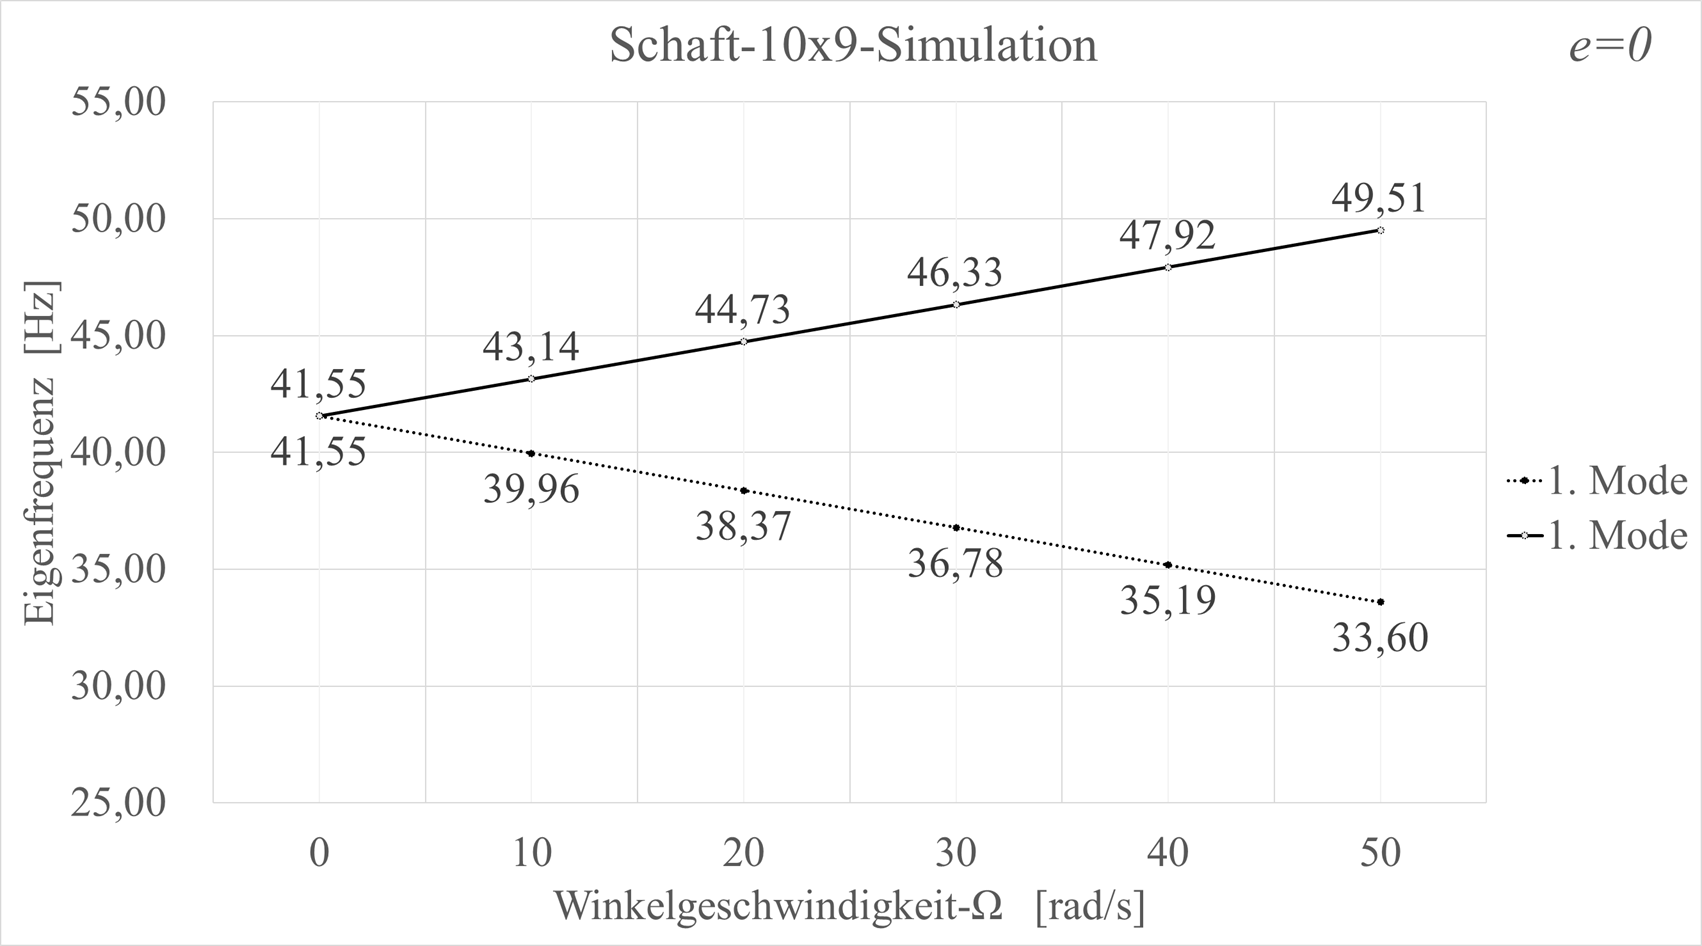
\includegraphics[width=0.95\linewidth, height=0.36\textheight]{Ergebnisse/Schaft_10x9_1Mode_Simu}
		\caption{Eigenfrequenzen vom 1. Biegemode in Abhängigkeit der Winkelgeschwindigkeit bei einem Exzentrizitätsfehler von $ e=0 $. Berechnungsparameter: Schaft $ 10\times9 $, $\rho = 7800 \,\text{kg}/\text{m}^{3} $, $ E=2,1\cdot 10^{11} \,\text{N}/\text{m}^{2} $, $ \nu=0,28 $.}
		\label{fig:Result-Schaft-10x9-Simulation-1-Mode}
	\end{figure}
	
	\begin{figure}[H]
		\centering
		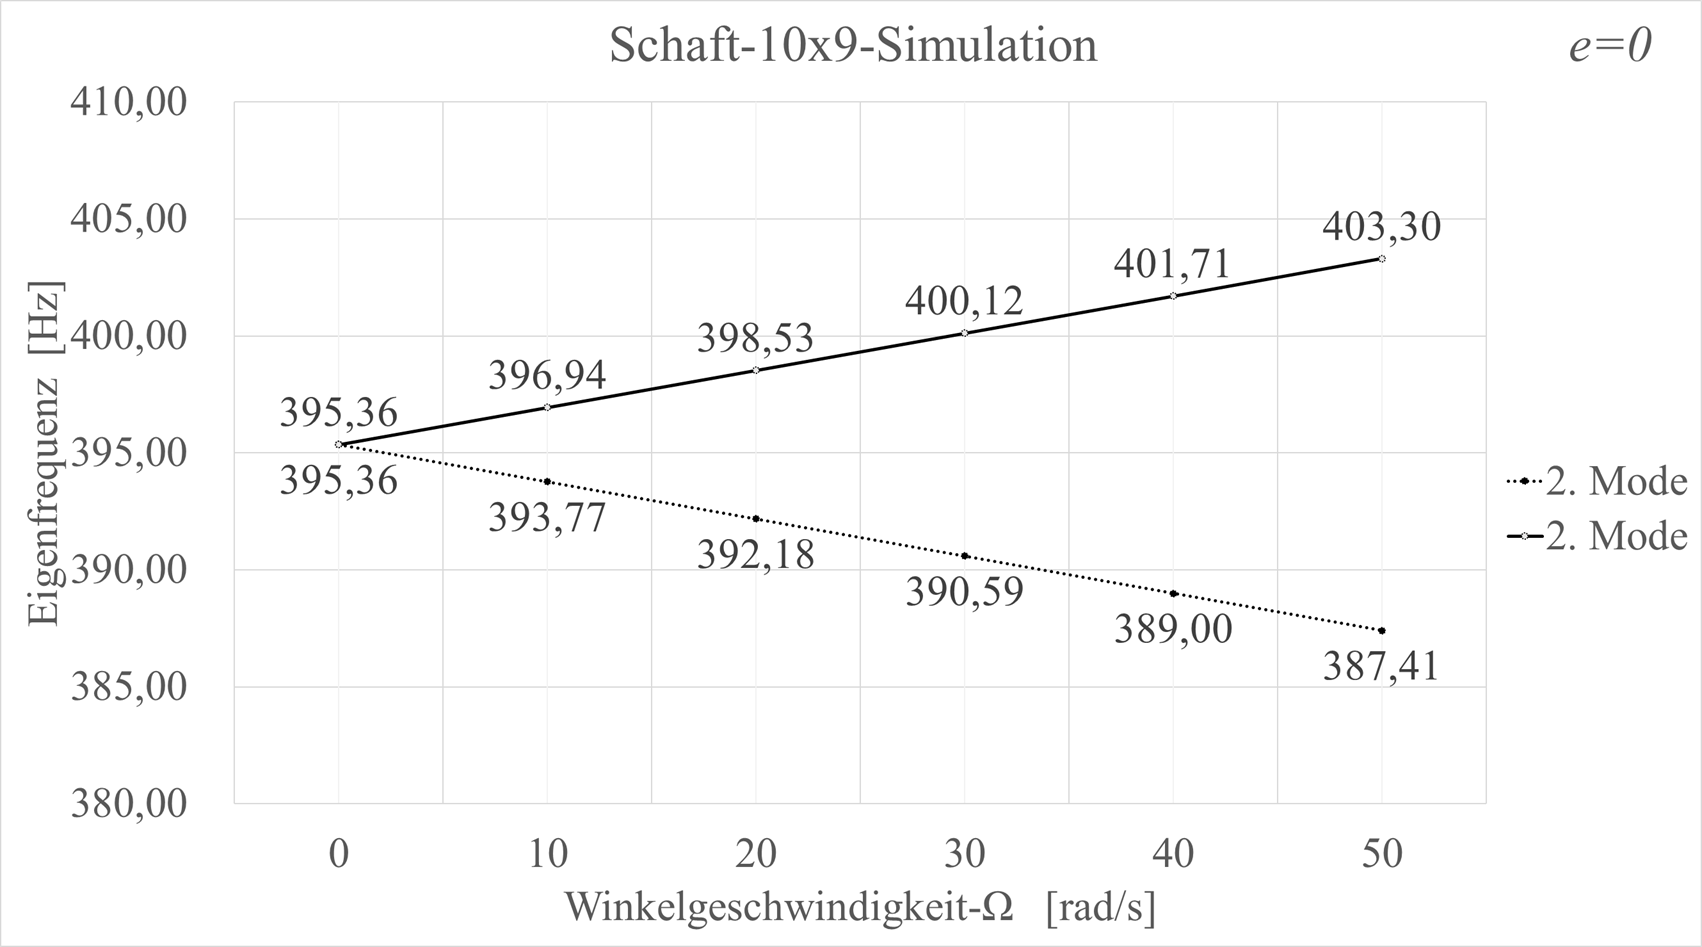
\includegraphics[width=0.95\linewidth, height=0.36\textheight]{Ergebnisse/Schaft_10x9_2Mode_Simu}
		\caption{Eigenfrequenzen vom 2. Biegemode in Abhängigkeit der Winkelgeschwindigkeit bei einem Exzentrizitätsfehler von $ e=0 $. Berechnungsparameter: Schaft $ 10\times9 $, $\rho = 7800 \,\text{kg}/\text{m}^{3} $, $ E=2,1\cdot 10^{11} \,\text{N}/\text{m}^{2} $, $ \nu=0,28 $.}
		\label{fig:Result-Schaft-10x9-Simulation-2-Mode}
	\end{figure}

	\begin{figure}[H]
		\centering
		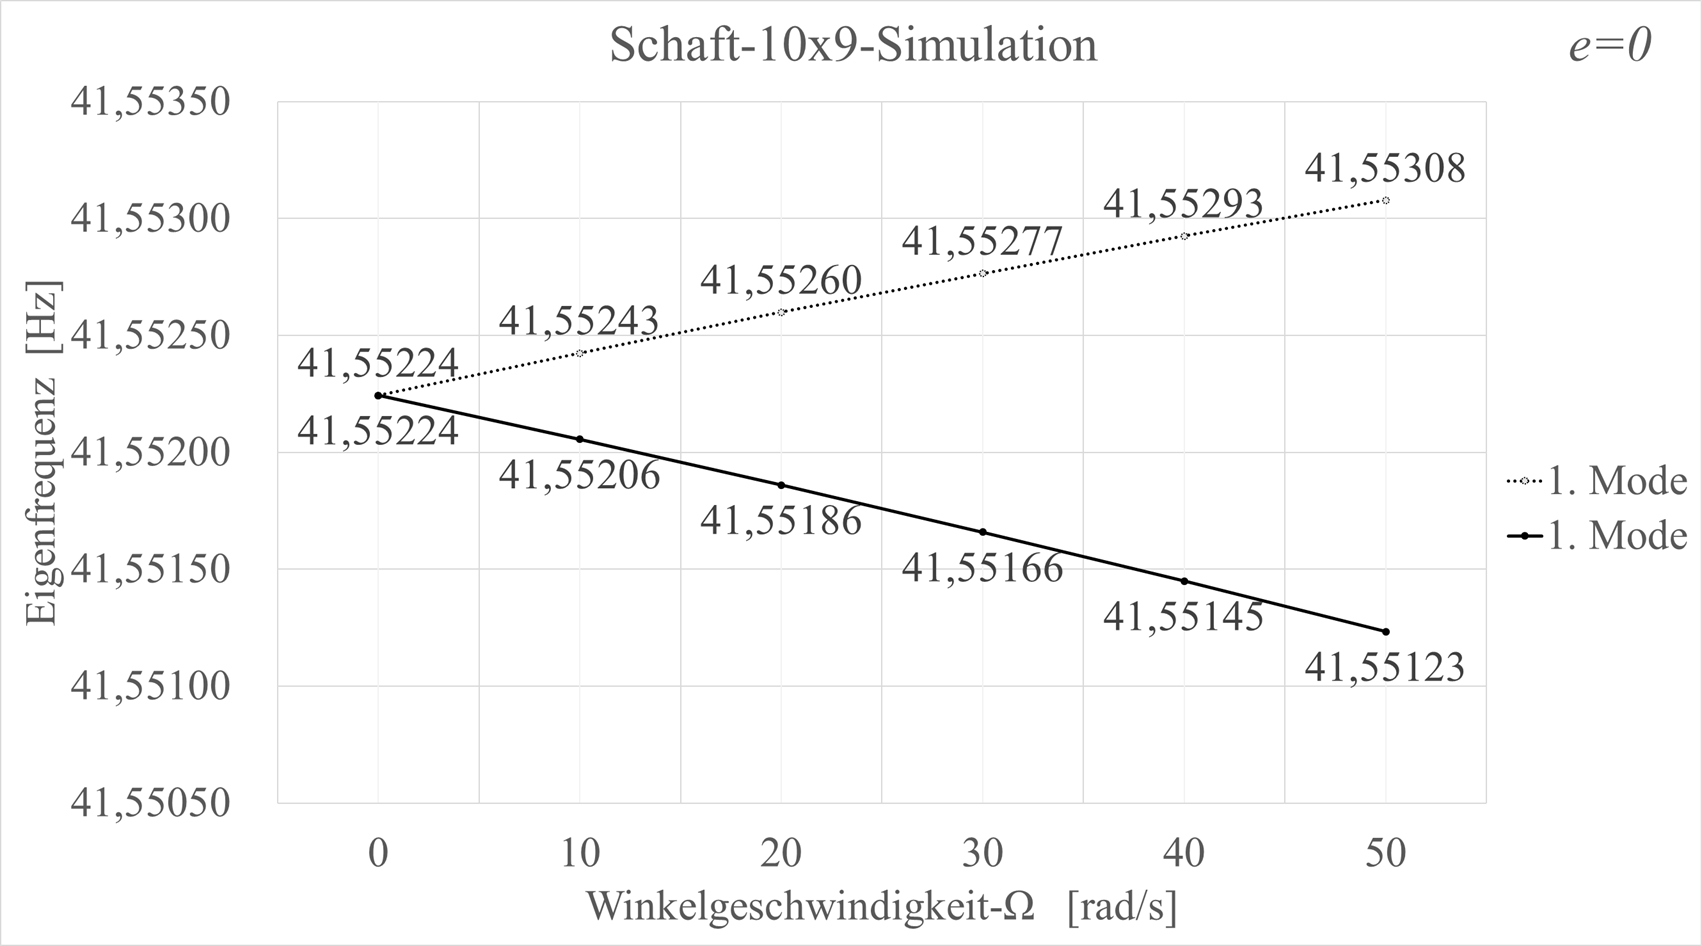
\includegraphics[width=0.95\linewidth, height=0.36\textheight]{Ergebnisse/Schaft_10x9_1Mode_Simu_ruhend}
		\caption{Eigenfrequenzen vom 1. Biegemode in Abhängigkeit der Winkelgeschwindigkeit bei einem Exzentrizitätsfehler von $ e=0 $ im ruhenden Inertialsystem. Berechnungsparameter: Schaft $ 10\times9 $, $\rho = 7800 \,\text{kg}/\text{m}^{3} $, $ E=2,1\cdot 10^{11} \,\text{N}/\text{m}^{2} $, $ \nu=0,28 $.}
		\label{fig:Result-Schaft-10x9-Simulation-1-Mode-ruhend}
	\end{figure}
	
	\begin{figure}[H]
		\centering
		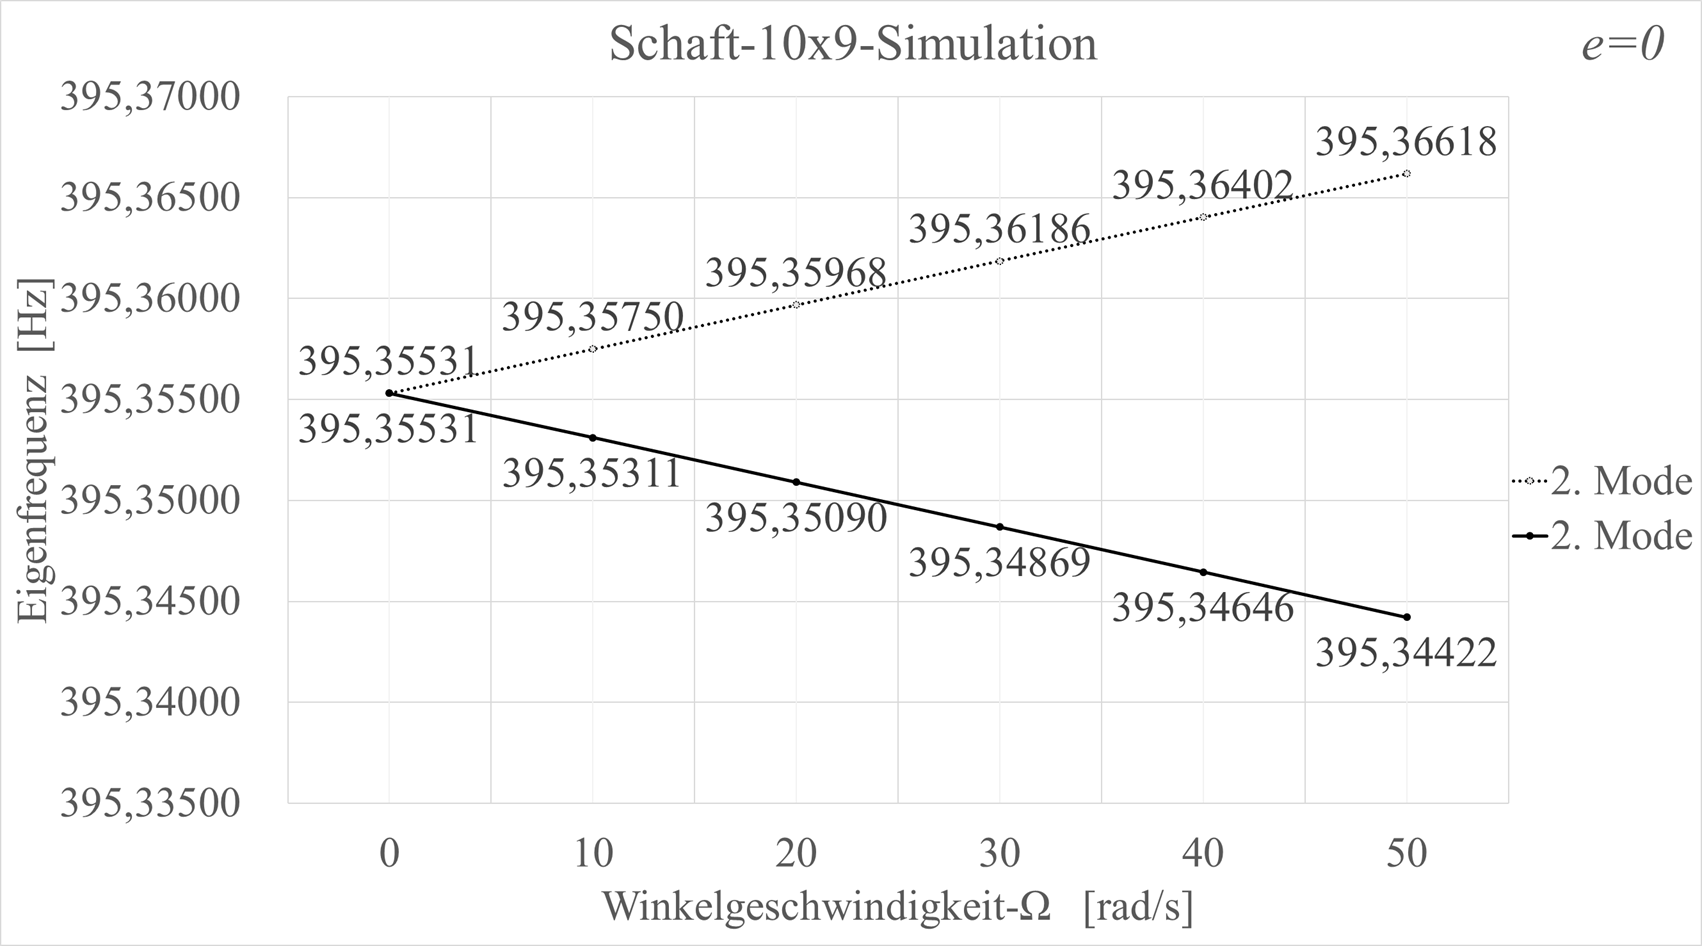
\includegraphics[width=0.95\linewidth, height=0.36\textheight]{Ergebnisse/Schaft_10x9_2Mode_Simu_ruhend}
		\caption{Eigenfrequenzen vom 2. Biegemode in Abhängigkeit der Winkelgeschwindigkeit bei einem Exzentrizitätsfehler von $ e=0 $ im ruhenden Inertialsystem. Berechnungsparameter: Schaft $ 10\times9 $, $\rho = 7800 \,\text{kg}/\text{m}^{3} $, $ E=2,1\cdot 10^{11} \,\text{N}/\text{m}^{2} $, $ \nu=0,28 $.}
		\label{fig:Result-Schaft-10x9-Simulation-2-Mode-ruhend}
	\end{figure}

	\begin{figure}[H]
		\centering
		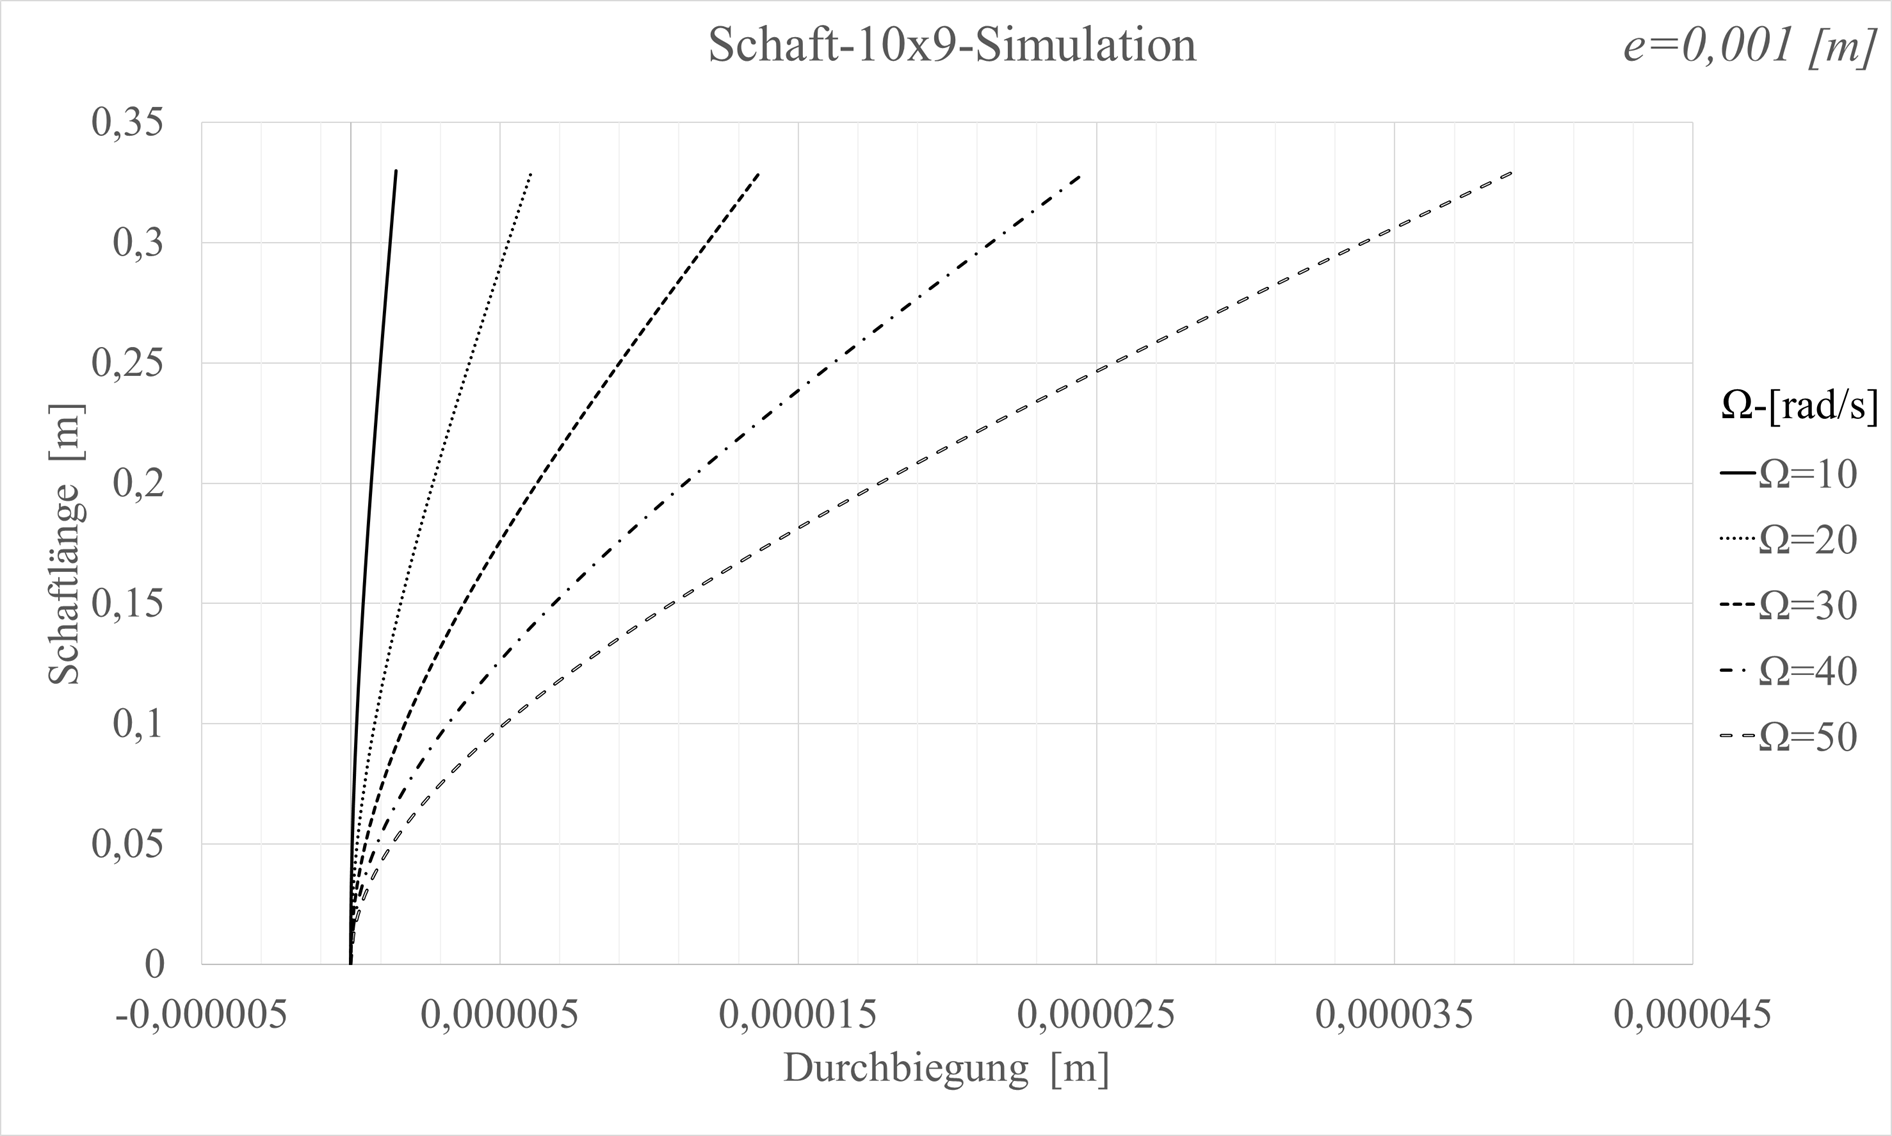
\includegraphics[width=0.95\linewidth, height=0.40\textheight]{Ergebnisse/Schaft_10x9_Biegung_Simu} 
		\caption{Durchbiegung in Abhängigkeit der Winkelgeschwindigkeit bei einem Exzentrizitätsfehler von $ e=0,001\,\text{m}$. Berechnungsparameter: Schaft $ 10\times9 $, $\rho = 7800 \,\text{kg}/\text{m}^{3} $, $ E=2,1\cdot 10^{11} \,\text{N}/\text{m}^{2} $, $ \nu=0,28 $.}
		\label{fig:Result-Schaft-10x9-Simulation-Durchbiegung}
	\end{figure}
	
	
	\begin{figure}[H]
		\centering
		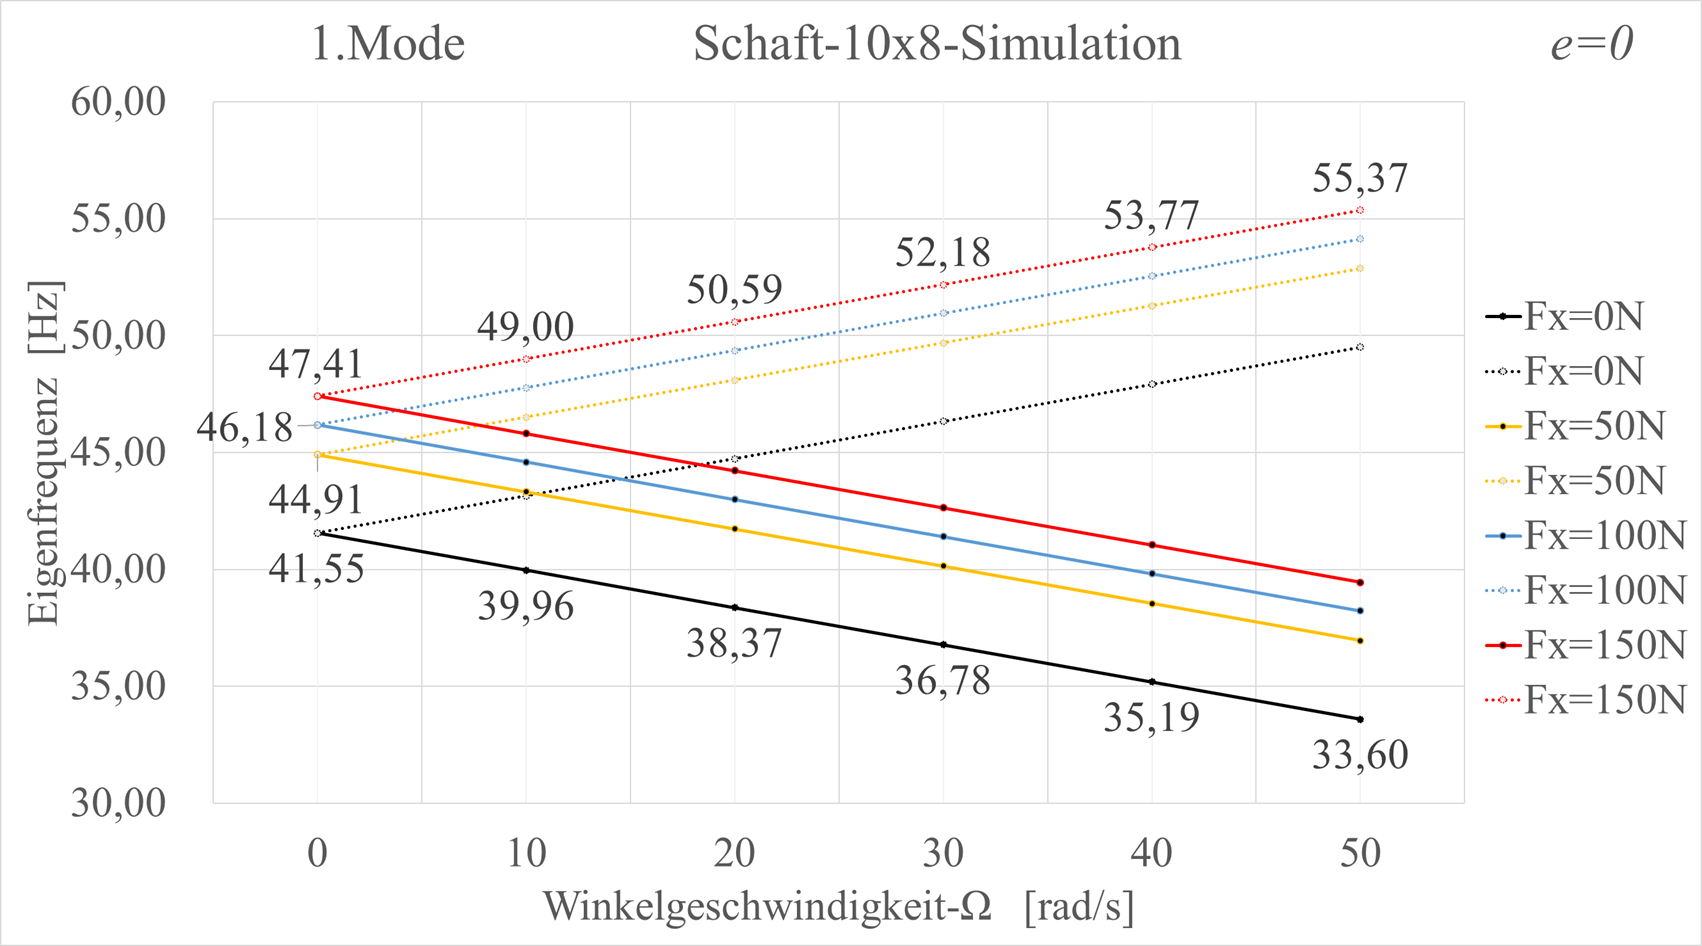
\includegraphics[width=0.95\linewidth, height=0.38\textheight]{Ergebnisse/Schaft_10x9_Zugkraft_Simu} 
		\caption{Eigenfrequenzen vom 1. Biegemode in Abhängigkeit der Winkelgeschwindigkeit $ \Omega $ und der Zugkraft $ Fx $ bei einem Exzentrizitätsfehler von $ e=0 $. Berechnungsparameter: Schaft $ 10\times9 $, $\rho = 7800 \,\text{kg}/\text{m}^{3} $, $ E=2,1\cdot 10^{11} \,\text{N}/\text{m}^{2} $, $ \nu=0,28 $.}
		\label{fig:Result-Schaft-10x9-Simulation-Zugkraft}
	\end{figure}


	
	\begin{figure}[H]
		\centering
		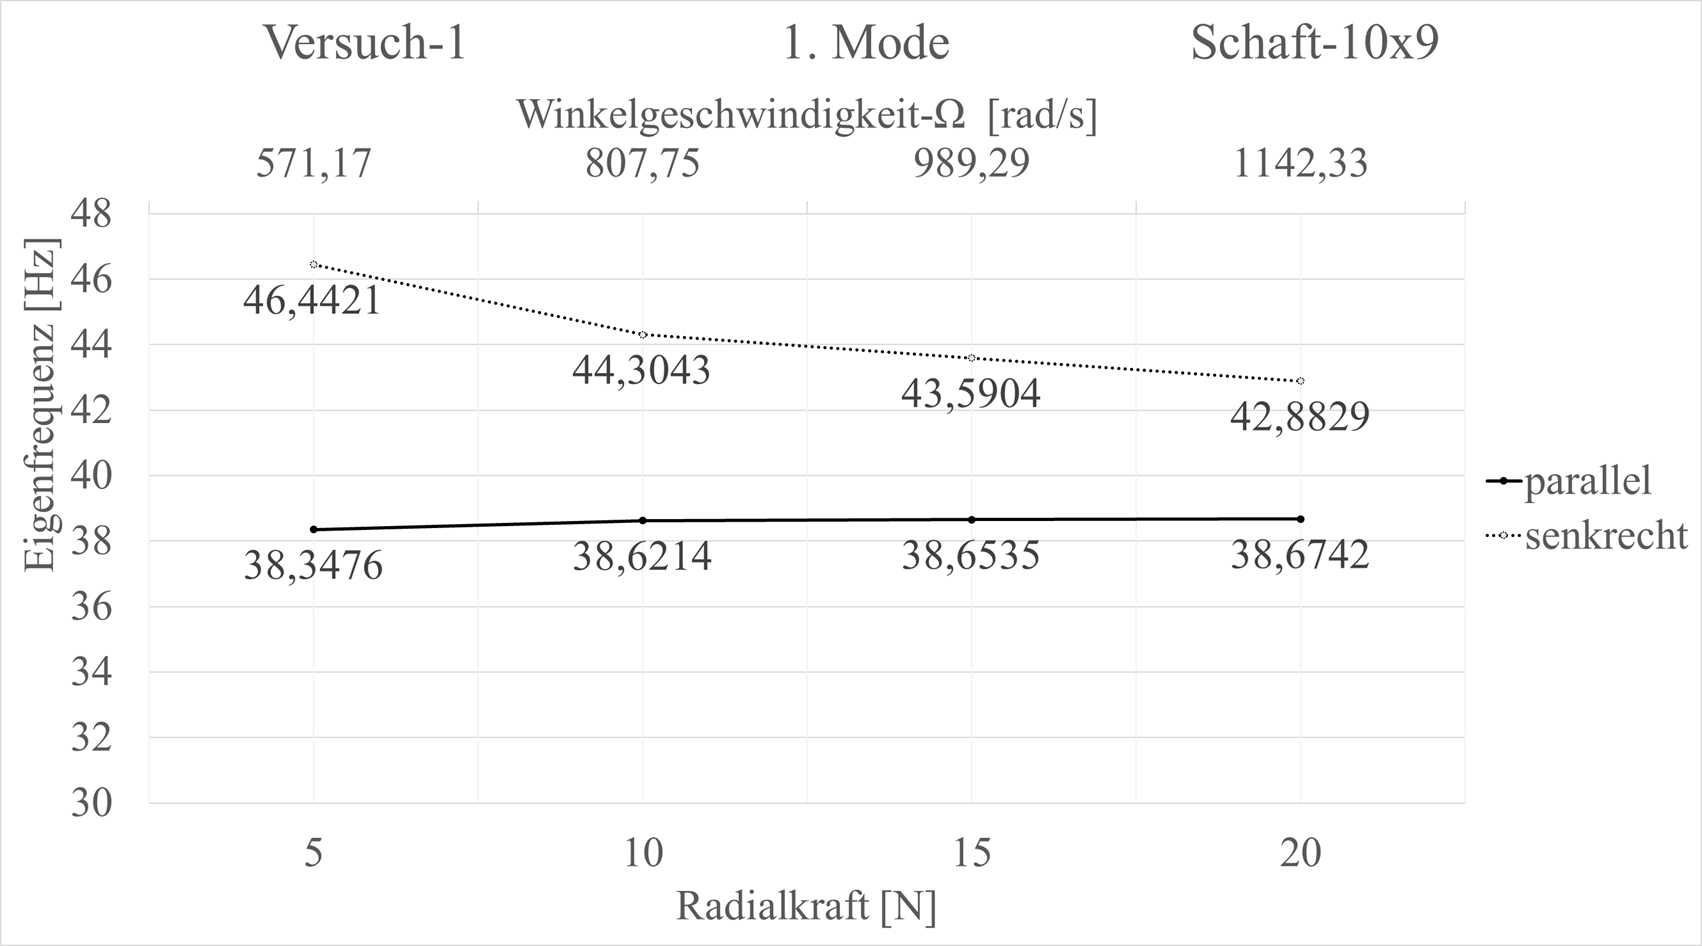
\includegraphics[width=0.95\linewidth, height=0.36\textheight]{Ergebnisse/Schaft_10x9_1Mode_ver1} 
		\caption{Gemessene Eigenfrequenzen vom 1. Biegemode in Abhängigkeit der Vorspannkraft. Angabe der Eigenfrequenzen parallel und senkrecht zur Vorspannrichtung (Probe Nr. 1 (Schaft $ 10\times9 $ ), Versuchsreihe 1).}
		\label{fig:Result-Schaft-10x9-1Mode-Ver1}
	\end{figure}
	
	\begin{figure}[H]
		\centering
		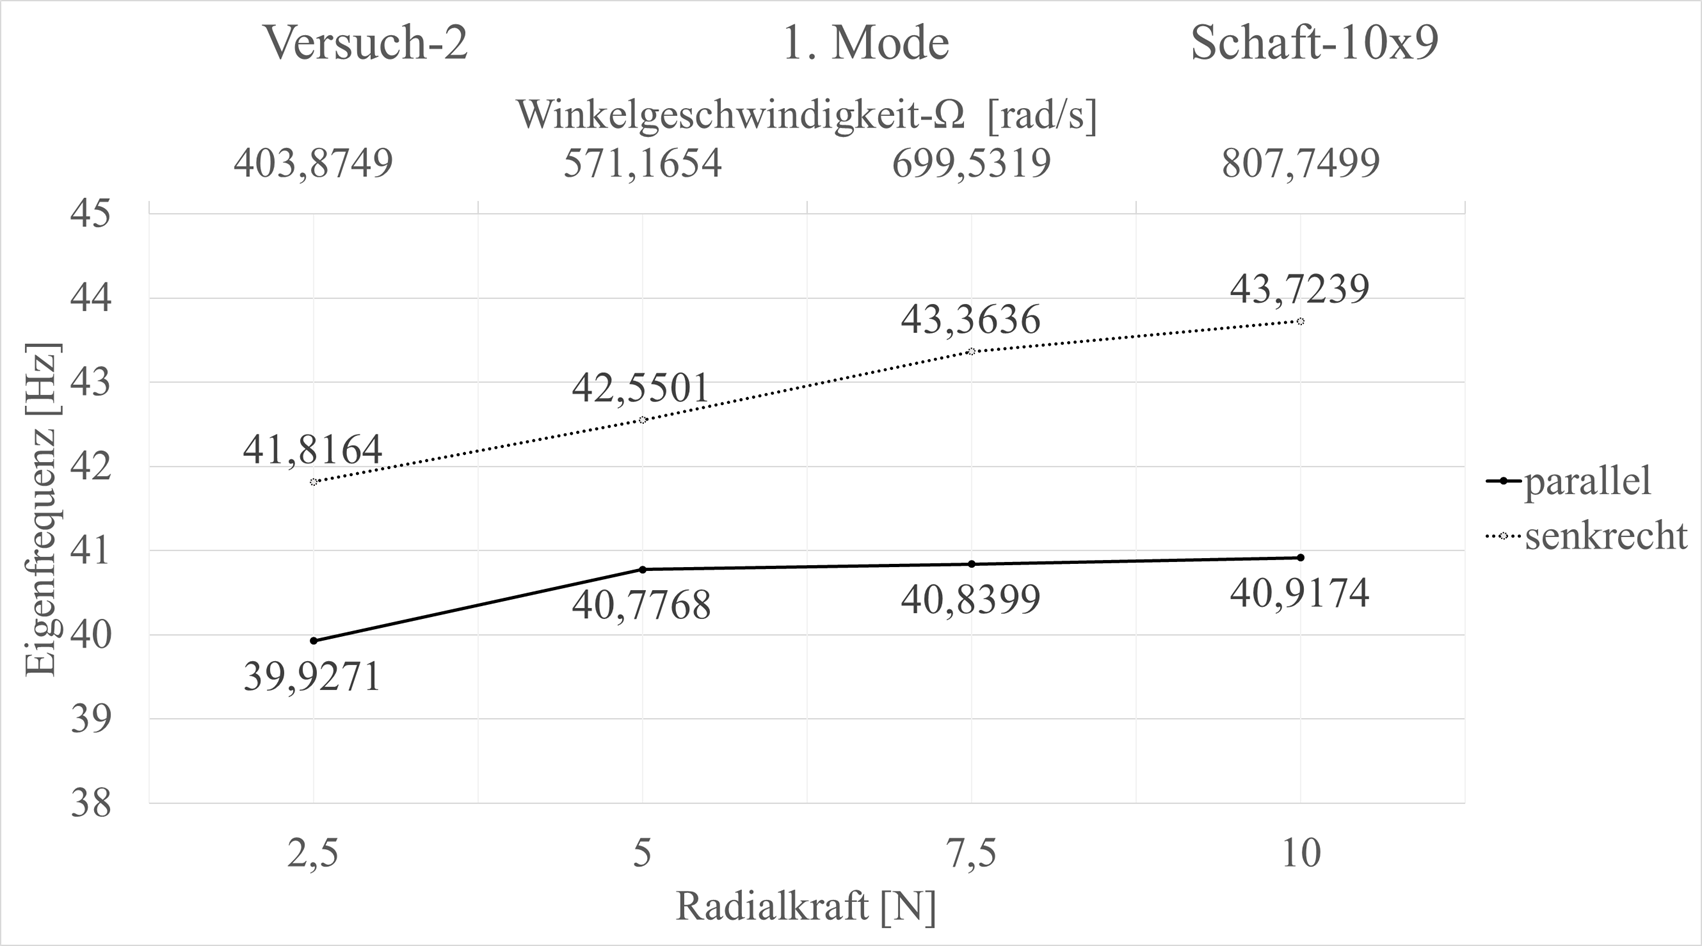
\includegraphics[width=0.95\linewidth, height=0.36\textheight]{Ergebnisse/Schaft_10x9_1Mode_ver2} 
		\caption{Gemessene Eigenfrequenzen vom 1. Biegemode in Abhängigkeit der Vorspannkraft. Angabe der Eigenfrequenzen parallel und senkrecht zur Vorspannrichtung (Probe Nr. 1 (Schaft $ 10\times9 $ ), Versuchsreihe 2).}
		\label{fig:Result-Schaft-10x9-1Mode-Ver2}
	\end{figure}

	\begin{figure}[H]
		\centering
		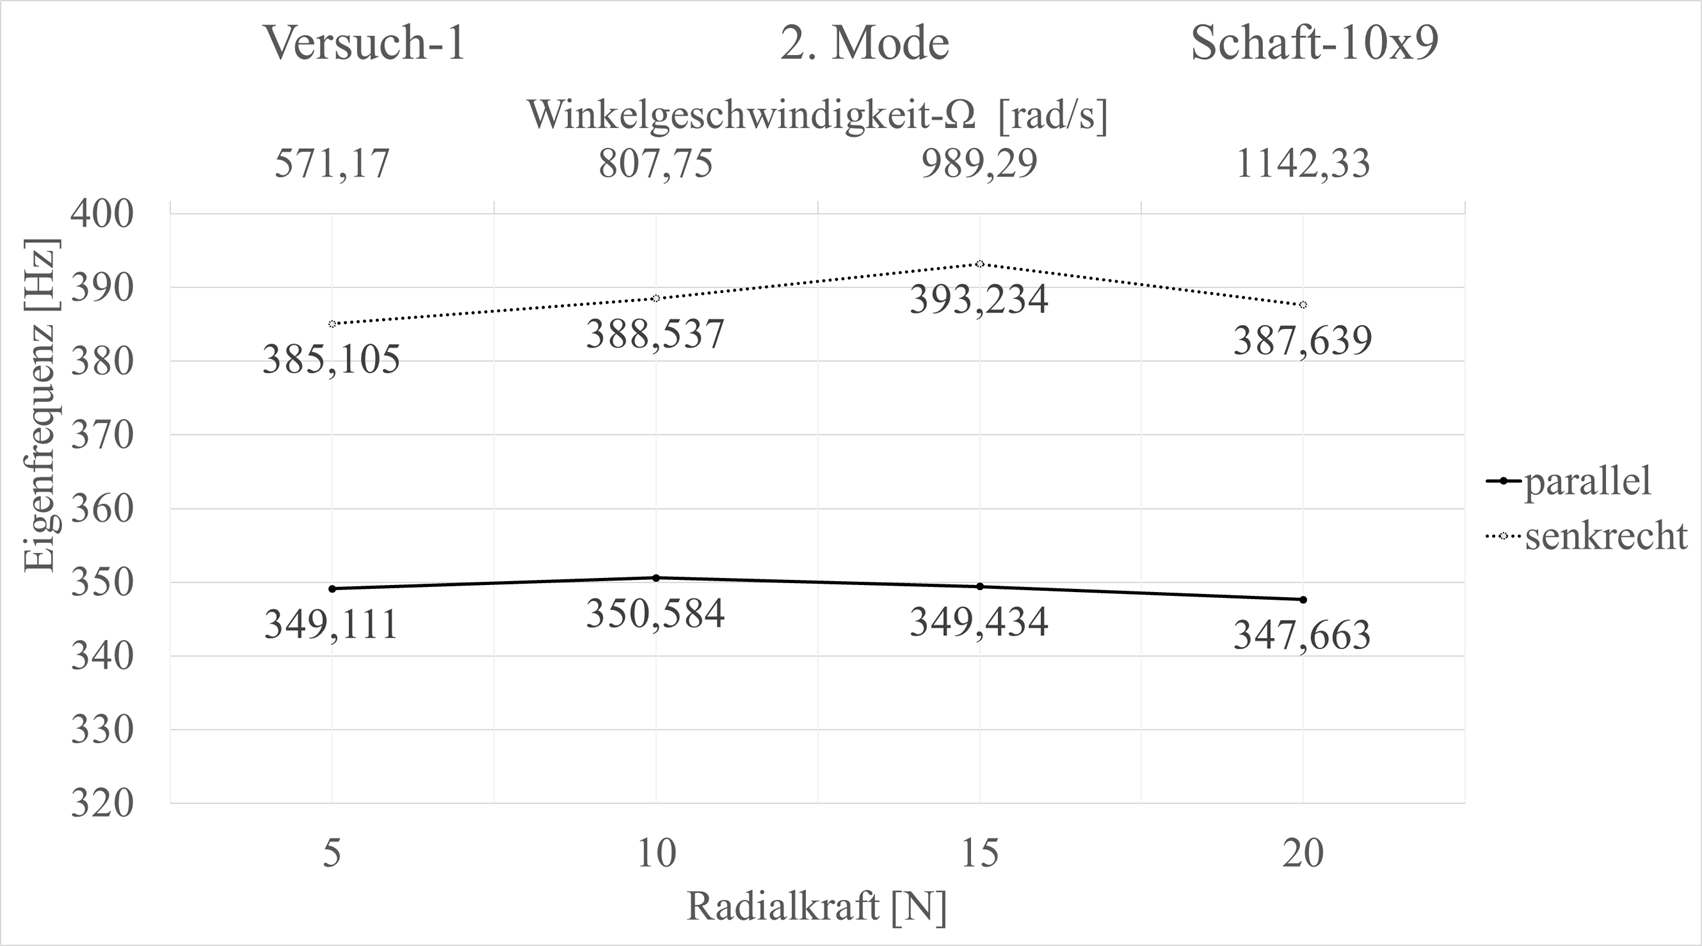
\includegraphics[width=0.95\linewidth, height=0.36\textheight]{Ergebnisse/Schaft_10x9_2Mode_ver1} 
		\caption{Gemessene Eigenfrequenzen vom 2. Biegemode in Abhängigkeit der Vorspannkraft. Angabe der Eigenfrequenzen parallel und senkrecht zur Vorspannrichtung (Probe Nr. 1 (Schaft $ 10\times9 $ ), Versuchsreihe 1).}
		\label{fig:Result-Schaft-10x9-2Mode-Ver1}
	\end{figure}

	\begin{figure}[H]
		\centering
		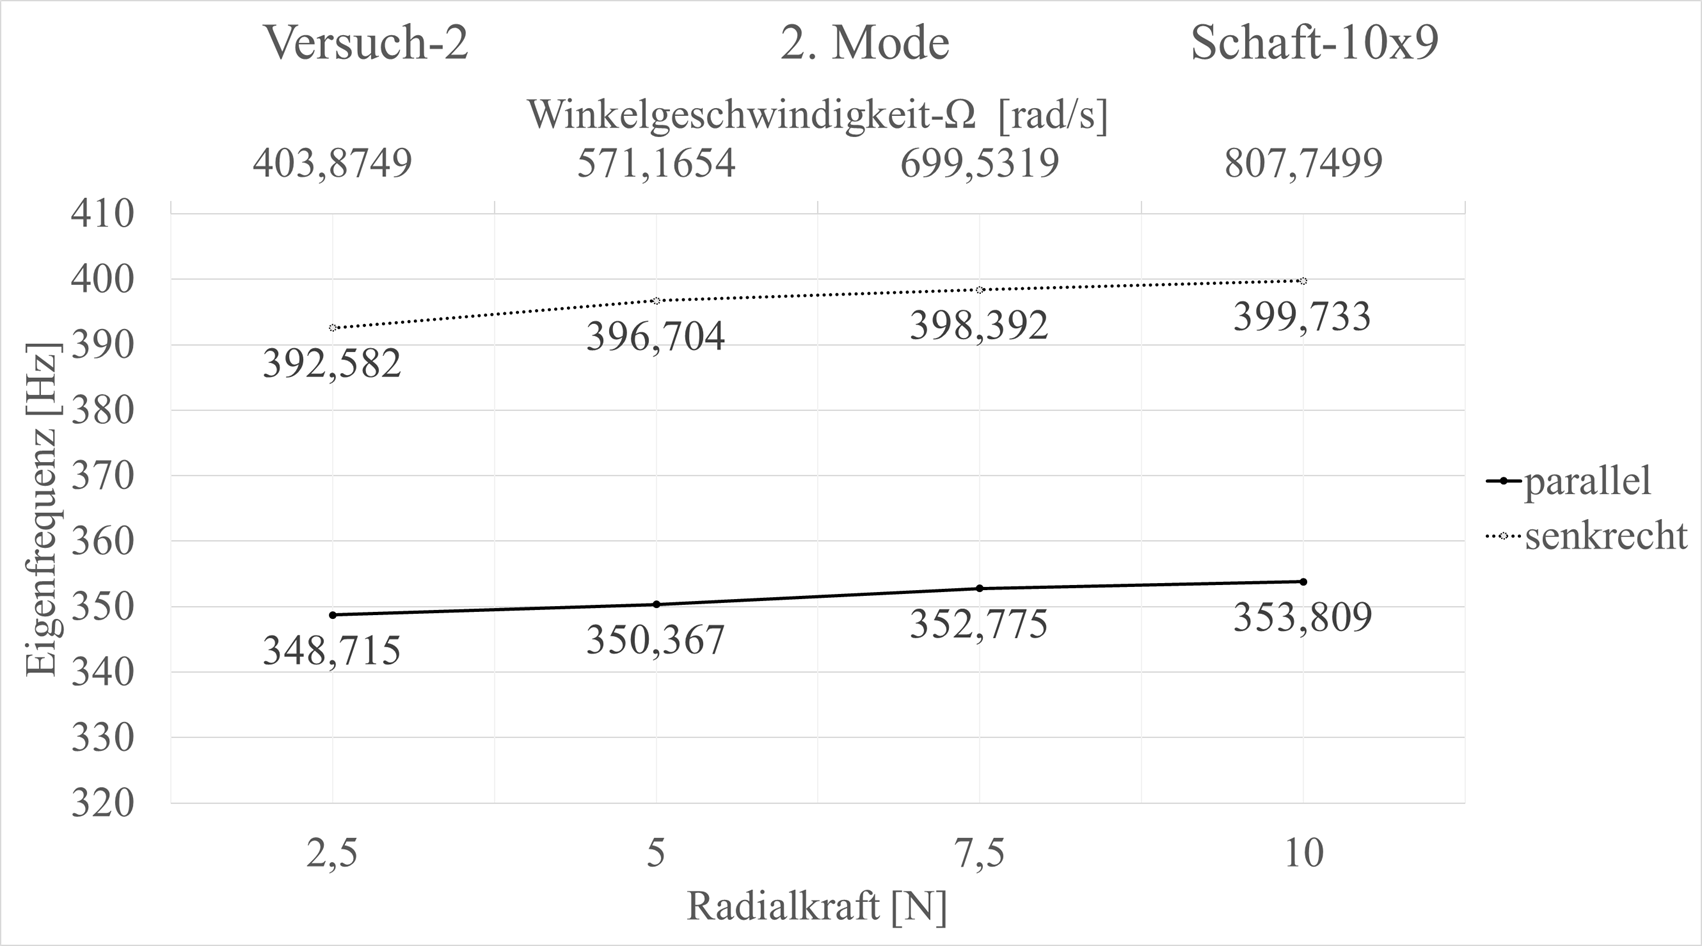
\includegraphics[width=0.95\linewidth, height=0.36\textheight]{Ergebnisse/Schaft_10x9_2Mode_ver2} 
		\caption{Gemessene Eigenfrequenzen vom 2. Biegemode in Abhängigkeit der Vorspannkraft. Angabe der Eigenfrequenzen parallel und senkrecht zur Vorspannrichtung (Probe Nr. 1 (Schaft $ 10\times9 $ ), Versuchsreihe 2).}
		\label{fig:Result-Schaft-10x9-2Mode-Ver2}
	\end{figure}

	 Der Einfluss der Vorspannkraft auf die Eigenfrequenzen ist ähnlich wie bei Probe 1. Die in den Abbildungen gezeigte Winkelgeschwindigkeit wurde wieder, mit einem konstanten Exzentrizitätsfehler von $ e=0,001\,\text{m}$, nach \ref{equ:Verhältnis-Rotaion-und-Radialkraft} berechnet. \\
	 Für den ersten Mode kann erneut eine tendenzielle Versteifung der Eigenfrequenzen festgestellt werden, wobei der Einfluss senkrecht zur Vorspannrichtung größer ist als parallel dazu. Gleiches gilt auch für die Eigenfrequenzen von Mode 2. Der relative Einfluss ist hier jedoch geringer.
	 Erneut sind die simulierten Eigenfrequenzen des ruhenden Schaft etwas höher als die gemessenen Werte. 
	 \\
	 Es ist ersichtlich, dass die experimentellen Ergebnisse eine gewisse Zufälligkeit aufweisen. Um genauere Ergebnisse zu erhalten müssten mehrere Messungen durchgeführt und diese dann gemittelt werden.
	
	

%% empty page %%%%%%%%%%%%%%%%%%%%%%%%%%%%%%%%%%%%%%%%%%
		%% empty page %%%%%%%%%%%%%%%%%%%%%%%%%%%%%%%%%%%%%%%%%%
	\newpage
	\pagestyle{empty}
	\ \\
	\newpage
	%%%%%%%%%%%%%%%%%%%%%%%%%%%%%%%%%%%%%%%%%%%%%%%%%%%%%%%%%
%%%%%%%%%%%%%%%%%%%%%%%%%%%%%%%%%%%%%%%%%%%%%%%%%%%%%%%%%%%%%%%%%%%%%%%%%%%%%%%%%%%%%%%%%%%%%%%%%%%%%%%%%%%%%%%%%%	
	
		\pagestyle{fancy}
	\section{Zusammenfassung und Ausblick} \label{sec:Zusammenfassung}
	In der vorliegenden Arbeit wird sowohl die numerische als auch die experimentelle Modalanalyse eines Werkzeugschaftes beim HSC-Fräsen beschrieben. Dabei werden die Auswirkungen von verschiedenen Parametern auf die Eigenfrequenzen des Schaftes analysiert. Wegen der hohen Rotationsgeschwindigkeit des Werkzeughalters wurde die simulative Modalanalyse durch eine nichtlinearen Finite-Elemente-Methode, in Kombination mit dem Prinzip von Hamilton, durchgeführt und mit \Matlab programmiert. Aufgrund des experimentellen Versuchsaufbaus mit dem kabelgebundenen Anregungshammer und dem Beschleunigungssensor ist es nicht möglich, Versuche unter Rotation durchzuführen. Deshalb wurde am oberen Ende des Werkzeugschafts eine Radialkraft eingeleitet, um die Wirkung der Rotation in Verbindung mit einer Exzentrizität nachzubilden.\\
	
	Zunächst werden die notwendigen theoretischen Grundlagen erklärt, um das Berechnungsmodell zur numerischen Simulation umzusetzen. Im Speziellen wird hierfür die nichtlineare Finite-Elemente-Methode verwendet. Anschließend werden die Eigenfrequenzen und Deformationen des Schaftes für verschiedene Parameter simuliert. Bei den Experimenten werden die niedrigsten Eigenfrequenzen in Abhängigkeit der Vorspannkraft (entspricht einem Exzentrizitätsfehler $e$ bei gleichzeitiger Rotation) ermittelt.\\
	
	Die Ergebnisse werden anschließend in einem separaten Kapitel ausgewertet. Beispielsweise zeigen die Simulationen eine Aufspaltung der Eigenfrequenzen durch die Rotation. Weiterhin ist eine schwache Abhängigkeit der Eigenfrequenzen von der Vorspannkraft bei den experimentellen Ergebnisse zu sehen. So wurde eine tendenzielle Versteifung für die Eigenfrequenzen des ersten Modes mit zunehmender Vorspannkraft festgestellt.\\
	
	Schließlich ist festzustellen, dass die ermittelten Erkenntnisse zur Konstruktion von schwingungsarmen Werkzeugschäften und deren Optimierung verwendet werden können. Für das weitere Vorgehen wird empfohlen, mehrere Messungen durchzuführen und die Ergebnisse anschließend zu mitteln. Damit können Messungenauigkeiten durch zufällige Störungen minimiert werden.
	
%% empty page %%%%%%%%%%%%%%%%%%%%%%%%%%%%%%%%%%%%%%%%%%
		%% empty page %%%%%%%%%%%%%%%%%%%%%%%%%%%%%%%%%%%%%%%%%%
	\newpage
	\pagestyle{empty}
	\ \\
	\newpage
	%%%%%%%%%%%%%%%%%%%%%%%%%%%%%%%%%%%%%%%%%%%%%%%%%%%%%%%%%
%%%%%%%%%%%%%%%%%%%%%%%%%%%%%%%%%%%%%%%%%%%%%%%%%%%%%%%%%%%%%%%%%%%%%%%%%%%%%%%%%%%%%%%%%%%%%%%%%%%%%%%%%%%%%%%%%%	
		\pagestyle{fancy}
	\section{Verzeichnis}
	\subsection{Quellenverzeichnis}
	%\nocite{*}
	\renewcommand\refname{\vskip -1cm}
	\bibliography{Masterarbeit}
	
	\subsection{Symbol- und Abkürzungsverzeichnis}
	
	\subsubsection*{Lateinische Notation}
	\begin{flalign*}
	& A       && \text{m}^{2}    && \text{Querschnittfläche}    && \\
%	& b       && \text{m}        && \text{Breit des Querschnitts}    && \\
%	& B       && \text{m}        && \text{Breit der Platte}    && \\
	& e       && \text{m}        && \text{Exzentrizitätsfehler} && \\
	& E       && \text{N}/\text{m}^{2} && \text{E-Modul} && \\
	& E_{kin} && \text{J}        && \text{kinetische Energie} && \\
	& E_{pot} && \text{J}        && \text{potentielle Energie} && \\
%	& f       && \mathrm{Hz}     && \text{Eigenfrequenz}    && \\
	& F       && \text{N}        && \text{Radialkraft}    && \\
	& Fx      && \text{N}        && \text{Zugkraft}    && \\
%	& h       && \text{m}        && \text{Höhe des Querschnitts}    && \\
	& H       && \text{m}        && \text{Übertragungsfunktion}    && \\
	& i       && -               && \text{Zählvariablen}    && \\
	& I       && \text{m}^{4}    && \text{Flächenträgheitsmoment}    && \\
	& I_{t}   && \text{m}^{4}    && \text{Torsionsträgheitsmoment} &&\\
	& L       && \text{m}        && \text{Länge des Schaftes}    && \\
	& l_{e}   && \text{m}        && \text{Länge eines Elements}    && \\
	& M_{b}   && \text{Nm}       && \text{Biegemoment}    && \\
	& t       && \text{s}        && \text{Zeit}    && \\
	& u       && \text{m}        && \text{Längsverschiebung in X-Richtung}    && \\
	& v       && \text{m}        && \text{Durchbiegung in Y-Richtung}    && \\
	& V		  && \text{m}^{3}    && \text{Volumen}    && \\
	& w       && \text{m}        && \text{Durchbiegung in Z-Richtung}    && \\
	& W		  && \text{J}        && \text{Formänderungsenergie}    && \\
	\end{flalign*}
	
	\subsubsection*{Griechische Notation}
	\begin{flalign*}
	& \varepsilon  && 1                       && \text{Dehnung}    && \\
	& \lambda      && -                       && \text{Eigenwert}    && \\
	& \nu          && 1                       && \text{Poissionzahl}    && \\
	& \rho         && \text{kg}/\text{m}^{3}  && \text{Dichte}    && \\
	& \phi         && 1 		              && \text{Verdrehung der Torsion}    &&\\
	& \varphi,\psi && 1 		              && \text{Biegewinkel}    &&\\
	& \Omega       && \text{rad/s} 		      && \text{Winkelgeschwindigkeit}    &&\\
	& \omega       && \text{1/s} 		      && \text{Kreisfrequenz}    &&\\
	\end{flalign*}
	
	
	\subsubsection*{Vektoren und Matrizen}
	\begin{flalign*}
	& \mathbf{D}      && \text{Dämpfungsmatrix}    && \\
	& \mathbf{D}_{e}  && \text{Dämpfungsmatrix eines Elements}    && \\
	& \vec{f}         && \text{Knotenkraftvektor}    && \\
	& \vec{f}_{e}     && \text{Knotenkraftvektor eines Elements}    && \\
	& \mathbf{K}      && \text{Steifigkeitsmatrix}    && \\
	& \mathbf{K}_{e}  && \text{Steifigkeitsmatrix eines Elements}    && \\
	& \mathbf{M}      && \text{Massenmatrix}    && \\
	& \mathbf{M}_{e}  && \text{Massenmatrix eines Elements}    && \\
	& \vec{N}         && \text{Vektor der Formfunktion}    && \\
%	& \vec{r}_{p}         && \text{Ortsvektor}    && \\
	& \mathbf{R}      && \text{Rotationsmatrix}    &&\\
	& \vec{x}         && \text{Knotenverschiebungsvektor}    && \\
	& \vec{x}_{e}         && \text{Knotenverschiebungsvektoreines Elements}    && \\
	\end{flalign*}
	
	\subsubsection*{Indices}
	\begin{flalign*}
	& ( \  )_{t} \ ; \ \dot{( \ )}                       && \text{Erste Ableitung nach der Zeit}    && \\
	& ( \ )_{tt} \ ; \ \ddot{( \ )}                      && \text{Zweite Ableitung nach der Zeit}    && \\
	& ( \ )^{\mathrm{T}}                                 && \text{Transposition der Matrix}    && \\
	& ( \ )_{x} \ ; \ ( \ )_{y} \ ; \ ( \ )_{z}      && \text{Erste Ableitung in Richtung X,Y,Z}    && \\
	& ( \ )_{xx} \ ; \ ( \ )_{yy} \ ; \ ( \ )_{zz}   && \text{Zweite Ableitung in Richtung X,Y,Z}    && \\
	\end{flalign*}
	
	\newpage
	
	\subsection{Abbildungsverzeichnis}
	\renewcommand\listfigurename{\vskip -1cm}
	\listoffigures
	
	\newpage
	
	\subsection{Tabellenverzeichnis}
	\renewcommand\listtablename{\vskip -1cm}
	\listoftables



		\pagestyle{fancy}
	\fancyhead[RO,LE]{Anhang A: Programme}
	\setcounter{page}{1} 
	\fancyhead[LO,RE]{A-\thepage}
	\addcontentsline{toc}{paragraph}{Anhang A: Programme}
	\section*{Anhang A: Programme}
	\subsection*{Hauptprogramm}
	\begin{lstlisting}
	clear
	close all
	%###########################################
	% main Program  Ver-7.3     08.06.2020  Qian Sun  
	%###########################################
	%% parameter
	E=2.1e11;         % N/m^2
	D0=0.01;           % Durchmesser m
	R=D0/2;
	d=0.0005;          % Wandstaeker m
	r=R-d;
	A=pi*(R^2-r^2);   % Flaeche m^2
	l=0.33;           % m
	rho=7800;         % Dichte in [kg/m^3]
	V0=A*l*rho;       % Volume [m^3]
	mu=rho*A;         % Massenbelegung in [kg/m]
	Nel=20;           % number of elements in bend
	Nno=Nel+1;        % number of nodes in bend in linear_ansatz
	% Nno=Nel*2+1;        % number of nodes in qudra-ansatz
	le=l/Nel;         % length of an element
	I=pi*(R^4-r^4)/4;  % Flaechentraegheitsmoment
	It=2*I;     % Torsionstraegheitsmoment
	v=0.28;                % Poissonzahl
	G=E/(2*(1+v));        % Schubmodul
	c=0;                  % Feder-Steifigkeit [N/m]
	m=0.0303;                % Masse  [kg]
	
	Omega=40;    % Drehgeschwindigkeit [rad/s]
	e=-0;      % Exzentrizitaet      [m]
	q=6;          % Freiheitsgrad
	
	Fx=50;                      % force [N]
	Fy=0;                      % force [N]
	Fz=0;                      % force [N]
	M=0;                       % moment [N*m]
	
	FVec= zeros(q*Nel,1);       % empty global force Vektor 
	FVec(end-5)=Fx;
	FVec(end-4)=Fy;
	FVec(end-2)=Fz;
	FVec(end)=M;
	
	uMat=[];
	vMat=[];
	vxMat=[];
	wMat=[];
	wxMat=[];
	
	%% define empty matrice
	Kt=zeros(Nno*q);  % empty global stiffnes-matrix 
	M=zeros(Nno*q);   % empty global mass-matrix 
	B=zeros(Nno*q);   
	Q=zeros(Nno*q);
	
	
	Ae=zeros(2*q,q*Nno,Nel);
	for ie=1:Nel
	for i=1:2*q
	Ae(i,q*(ie-1)+i,ie)=1;
	end
	end
	
	u=zeros(Nno,1);
	w=zeros(Nno,1);
	v=zeros(Nno,1);
	wx=zeros(Nno,1);
	vx=zeros(Nno,1);
	phi=zeros(Nno,1);
	
	Nloop=5;
	Ux=0;
	Vx=0;
	Wx=0;
	
	%% main program
	for j=1:Nloop
	
	if j==1
	
	for k=1:Nel                                      % loop over every element
	[Kte,Me,Be,Qe,Ce,MeM,KteM,BeM,QeM] = Elementroutine_n_linear(A,E,rho,le,Ux,Vx,Wx,I,It,G,Omega,e,c,m);
	if k==Nel
	Kt=Kt+Ae(:,:,k)'*Kte*Ae(:,:,k)+Ae(:,:,k)'*Ce*Ae(:,:,k)+Ae(:,:,k)'*KteM*Ae(:,:,k);
	M =M+Ae(:,:,k)'*Me*Ae(:,:,k)+Ae(:,:,k)'*MeM*Ae(:,:,k);              
	B =B+Ae(:,:,k)'*Be*Ae(:,:,k)+Ae(:,:,k)'*BeM*Ae(:,:,k);
	Q =Q+Ae(:,:,k)'*Qe*Ae(:,:,k)+Ae(:,:,k)'*QeM*Ae(:,:,k);
	else
	Kt=Kt+Ae(:,:,k)'*Kte*Ae(:,:,k);             % place the distribution of every element to right place in global stiffnes-matrix
	M =M+Ae(:,:,k)'*Me*Ae(:,:,k);               % place the distribution of every element to right place in global mass-matrix
	B =B+Ae(:,:,k)'*Be*Ae(:,:,k);
	Q =Q+Ae(:,:,k)'*Qe*Ae(:,:,k);
	end
	end
	
	
	else
	
	for k=1:Nel                                     % loop over every element
	
	%                                  Ux=Fx/E/A;
	%                                  Vx=(vx(k+1)+vx(k))/2;
	%                                  Wx=(wx(k+1)+wx(k))/2;
	%            
	Ux=(u(k+1)-u(k))/le;
	Wx=(w(k+1)-w(k))/le;
	Vx=(v(k+1)-v(k))/le;
	[Kte,Me,Be,Qe,Ce,MeM,KteM,BeM,QeM] = Elementroutine_n_linear(A,E,rho,le,Ux,Vx,Wx,I,It,G,Omega,e,c,m);
	if k==Nel
	Kt=Kt+Ae(:,:,k)'*Kte*Ae(:,:,k)+Ae(:,:,k)'*Ce*Ae(:,:,k)+Ae(:,:,k)'*KteM*Ae(:,:,k);
	M =M+Ae(:,:,k)'*Me*Ae(:,:,k)+Ae(:,:,k)'*MeM*Ae(:,:,k);               % place the distribution of every element to right place in global mass-matrix
	B =B+Ae(:,:,k)'*Be*Ae(:,:,k)+Ae(:,:,k)'*BeM*Ae(:,:,k);
	Q =Q+Ae(:,:,k)'*Qe*Ae(:,:,k)+Ae(:,:,k)'*QeM*Ae(:,:,k);
	else
	Kt=Kt+Ae(:,:,k)'*Kte*Ae(:,:,k);             % place the distribution of every element to right place in global stiffnes-matrix
	M =M+Ae(:,:,k)'*Me*Ae(:,:,k);               % place the distribution of every element to right place in global mass-matrix
	B =B+Ae(:,:,k)'*Be*Ae(:,:,k);
	Q =Q+Ae(:,:,k)'*Qe*Ae(:,:,k);
	end
	end
	end
	
	for zz=1:q
	Kt(1,:) = [];
	Kt(:,1) = [];
	M(1,:) = [];
	M(:,1) = [];
	B(1,:) = [];
	B(:,1) = [];
	end
	
	QVec=diag(Q);
	QVec(1:q)=[];
	
	AVec=FVec+QVec;
	
	P=Kt\AVec;
	for yy=1:q
	P=[0;P];
	end
	
	for xx=1:Nno
	n=(xx-1)*q+1;
	u(xx)=P(n);
	w(xx)=P(n+1);
	wx(xx)=P(n+2);
	v(xx)=P(n+3);
	vx(xx)=P(n+4);
	phi(xx)=P(n+5);
	end
	
	if j==Nloop
	
	else
	Kt= zeros(q*Nno);                               % empty global stiffnes-matrix 
	M = zeros(q*Nno);                                % empty global mass-matrix 
	B = zeros(q*Nno);   
	Q = zeros(q*Nno);
	end
	
	% uMat=[uMat,u];
	% vMat=[vMat,v];
	% vxMat=[vxMat,vx];
	% wMat=[wMat,w];
	% wxMat=[wxMat,wx];
	
	end
	
	%%
	% define system-matrix
	null=zeros(size(M));
	Eins = eye(size(M));
	SysMat=[null,Eins; -inv(M)*Kt,-inv(M)*B];
	
	[V,D]=eig(SysMat);
	
	temp_d = diag(D);
	org_d = temp_d;
	for i=1:Nel*6
	temp_d(i,:)=[];
	end
	
	[nd, sortindex] = sort(temp_d);
	temp_v = V(:,sortindex);
	temp_f = -imag(nd)/(2*pi);
	
	%%
	lVec = zeros (Nno, 1);     % vector with node coordinates
	
	for k = 1: Nno
	lVec(k)=l/Nel*(k-1);
	end
	
	
	%% plot
	
	figure('Name','Programm')
	grid on
	
	subplot(1,3,1)
	plot(lVec,u);
	title('u(x)')
	subplot(1,3,2)
	plot(lVec,w);
	title('w(x)')
	subplot(1,3,3)
	plot(lVec,v);
	title('v(x)')
	\end{lstlisting}
	
	\subsubsection*{Elementroutine}
	\begin{lstlisting}
	%###########################################
	% Elementroutine  Ver-7.3     08.06.2020  Qian Sun
	%###########################################
	function [Kte,Me,Be,Qe,Ce,MeM,KteM,BeM,QeM] = Elementroutine_n_linear(A,E,rho,le,Ux,Vx,Wx,I,It,G,Omega,e,c,m)
	% Elementroutine: compute Kte, Me
	
	%%
	% define empty Matrix
	Kteux=zeros(12);
	Ktev=zeros(12);
	Ktevx=zeros(12); 
	Ktevxx=zeros(12);
	Ktew=zeros(12);
	Ktewx=zeros(12); 
	Ktewxx=zeros(12);
	Ktephi=zeros(12);
	Ktephix=zeros(12);
	
	Me=zeros(12);
	
	Be=zeros(12);
	Qe=zeros(12,1);
	
	
	%%
	xiVec=[-sqrt(3/7+2/7*sqrt(6/5)),-sqrt(3/7-2/7*sqrt(6/5)),sqrt(3/7-2/7*sqrt(6/5)),sqrt(3/7+2/7*sqrt(6/5))]; % define sampling points for Gauss-quadrature  
	wVec=[(18-sqrt(30))/36,(18+sqrt(30))/36,(18+sqrt(30))/36,(18-sqrt(30))/36];    % weights for sampling points of Gauss-quadrature 
	%%
	
	for i=1:length(xiVec)
	xi=xiVec(i);
	w =wVec(i);
	
	% define N, Nx, Nxx vector linear 
	N=[0.5-xi/2, 0, 0, 0, 0, 0, 0.5+xi/2, 0, 0, 0, 0, 0; ...
	0, 1/2-(3*xi)/4+(xi^3)/4, 1/4-xi/4-(xi^2)/4+(xi^3)/4, 0, 0, 0, 0, 1/2+(3*xi)/4-(xi^3)/4, -1/4-xi/4+(xi^2)/4+(xi^3)/4, 0, 0, 0; ...
	0, -3/4+(3*xi^2)/4, -1/4-xi/2+(3*xi^2)/4, 0, 0, 0, 0, 3/4-(3*xi^2)/4, -1/4+xi/2+(3*xi^2)/4, 0, 0, 0; ...
	0, 0, 0, 1/2-(3*xi)/4+(xi^3)/4, 1/4-xi/4-(xi^2)/4+(xi^3)/4, 0, 0, 0, 0, 1/2+(3*xi)/4-(xi^3)/4, -1/4-xi/4+(xi^2)/4+(xi^3)/4, 0; ...
	0, 0, 0, -3/4+(3*xi^2)/4, -1/4-xi/2+(3*xi^2)/4, 0, 0, 0, 0, 3/4-(3*xi^2)/4, -1/4+xi/2+(3*xi^2)/4, 0; ...
	0, 0, 0, 0,  0, 0.5-xi/2, 0, 0,  0,  0,  0, 0.5+xi/2];
	
	Nx=[-0.5, 0, 0,0, 0, 0, 0.5, 0, 0, 0, 0, 0; ...
	0, -3/4+(3*xi^2)/4, -1/4-xi/2+(3*xi^2)/4, 0, 0, 0,   0, 3/4-(3*xi^2)/4, -1/4+xi/2+(3*xi^2)/4, 0, 0, 0; ...
	0, 3*xi/2, -1/2+3*xi/2, 0, 0, 0, 0, -3*xi/2, 1/2+3*xi/2, 0, 0, 0; ...
	0, 0, 0, -3/4+(3*xi^2)/4,  -1/4-xi/2+(3*xi^2)/4, 0, 0, 0, 0, 3/4-(3*xi^2)/4, -1/4+xi/2+(3*xi^2)/4, 0; ...
	0, 0, 0, 3*xi/2, -1/2+3*xi/2, 0, 0, 0, 0, -3*xi/2, 1/2+3*xi/2, 0; ...
	0, 0, 0, 0, 0, -0.5, 0, 0, 0, 0, 0, 0.5]*(2/le);
	
	Nxx=[0, 0, 0, 0, 0, 0, 0, 0, 0, 0, 0, 0; ...
	0, 3*xi/2, -1/2+3*xi/2, 0, 0, 0, 0, -3*xi/2, 1/2+3*xi/2, 0, 0, 0; ...
	0, 3/2, 3/2, 0, 0, 0, 0, -3/2, 3/2, 0, 0, 0; ...
	0, 0, 0, 3*xi/2, -1/2+3*xi/2, 0, 0, 0, 0, -3*xi/2, 1/2+3*xi/2, 0; ...
	0, 0, 0, 3/2, 3/2, 0, 0, 0, 0, -3/2, 3/2, 0; ...
	0, 0, 0, 0, 0, 0, 0, 0, 0, 0, 0, 0]*((2/le)^2);
	
	Nu=N(1,:);
	Nw=N(2,:);
	Nv=N(4,:);
	Nphi=N(6,:);
	
	Nux=Nx(1,:);
	Nwx=Nx(2,:);
	Nvx=Nx(4,:);
	Nphix=Nx(6,:);
	
	Nuxx=Nxx(1,:);
	Nwxx=Nxx(2,:);
	Nvxx=Nxx(4,:);
	Nphixx=Nxx(6,:);
	
	% compute Kte, Me, Be, Qe for sampling point of Gauss-integration
	Me=Me + w*( rho*A*( (Nu'*Nu) + (Nv'*Nv) + (Nw'*Nw) ) + rho*I*( (Nvx'*Nvx)+(Nwx'*Nwx)+2*(Nphi'*Nphi) ) )*le/2;
	
	Be=Be+w*( 2*rho*A*Omega*( (Nv'*Nw) - (Nw'*Nv)))*le/2;
	
	Qe=Qe+w*(-rho*A*e*Omega^2*Nv')*le/2;
	%%
	Kteux=Kteux+w*A*E*((1+3*Ux+1.5*Ux^2+0.5*Vx^2+0.5*Wx^2)*Nux+(Vx+Vx*Ux)*Nvx+(Wx+Wx*Ux)*Nwx)'*Nux;
	Ktev=Ktev+w*rho*A*Omega^2*(-Nv'*Nv);
	Ktevx=Ktevx+w*A*E*((Vx+Vx*Ux)*Nux+(Ux+0.5*Ux^2+1.5*Vx^2+0.5*Wx^2)*Nvx+Vx*Wx*Nwx)'*Nvx;
	Ktevxx=Ktevxx+w*E*I*(Nvxx'*Nvxx);
	Ktew=Ktew+w*rho*A*Omega^2*(-Nw'*Nw);
	Ktewx=Ktewx+w*A*E*((Wx+Wx*Ux)*Nux+Vx*Wx*Nvx+(Ux+0.5*Ux^2+0.5*Vx^2+1.5*Wx^2)*Nwx)'*Nwx;
	Ktewxx=Ktewxx+w*E*I*(Nwxx'*Nwxx);
	Ktephi=Ktephi+w*rho*I*2*(-Nphix'*Nphix)*Omega^2;
	Ktephix=Ktephix+w*(G*It*Nphix)'*Nphix;
	
	end
	
	Kte=(Kteux+Ktev+Ktevx+Ktevxx+Ktew+Ktewx+Ktewxx+Ktephi+Ktephix)*le/2;
	Qe=diag(Qe);
	
	%% Ce, MeM, KteM
	xi=1;
	N=[ 0.5-xi/2, 0, 0, 0, 0, 0, 0.5+xi/2, 0, 0, 0, 0, 0; ...
	0, 1/2-(3*xi)/4+(xi^3)/4, 1/4-xi/4-(xi^2)/4+(xi^3)/4, 0, 0, 0, 0, 1/2+(3*xi)/4-(xi^3)/4, -1/4-xi/4+(xi^2)/4+(xi^3)/4, 0, 0, 0; ...
	0, -3/4+(3*xi^2)/4, -1/4-xi/2+(3*xi^2)/4, 0, 0, 0, 0, 3/4-(3*xi^2)/4, -1/4+xi/2+(3*xi^2)/4, 0, 0, 0; ...
	0, 0, 0, 1/2-(3*xi)/4+(xi^3)/4, 1/4-xi/4-(xi^2)/4+(xi^3)/4, 0, 0, 0, 0, 1/2+(3*xi)/4-(xi^3)/4, -1/4-xi/4+(xi^2)/4+(xi^3)/4, 0; ...
	0, 0, 0, -3/4+(3*xi^2)/4, -1/4-xi/2+(3*xi^2)/4, 0, 0, 0, 0, 3/4-(3*xi^2)/4, -1/4+xi/2+(3*xi^2)/4, 0; ...
	0, 0, 0, 0, 0, 0.5-xi/2, 0, 0, 0, 0, 0, 0.5+xi/2];
	
	Nu=N(1,:);
	Nw=N(2,:);
	Nv=N(4,:);
	
	MeM=m*( (Nu'*Nu) + (Nv'*Nv) + (Nw'*Nw) );
	
	BeM=2*m*Omega*( (Nv'*Nw) - (Nw'*Nv));
	
	QeM=-m*e*Omega^2*Nv';
	QeM=diag(QeM);
	
	Ce=c*(Nv'*Nv);
	
	KtevM=m*Omega^2*(-Nv'*Nv);
	KtewM=m*Omega^2*(-Nw'*Nw);
	
	KteM=KtevM+KtewM;
	
	end
	\end{lstlisting}
	
	
%% empty page %%%%%%%%%%%%%%%%%%%%%%%%%%%%%%%%%%%%%%%%%%
		%% empty page %%%%%%%%%%%%%%%%%%%%%%%%%%%%%%%%%%%%%%%%%%
	\newpage
	\pagestyle{empty}
	\ \\
	\newpage
	%%%%%%%%%%%%%%%%%%%%%%%%%%%%%%%%%%%%%%%%%%%%%%%%%%%%%%%%%
%%%%%%%%%%%%%%%%%%%%%%%%%%%%%%%%%%%%%%%%%%%%%%%%%%%%%%%%%%%%%%%%%%%%%%%%%%%%%%%%%%%%%%%%%%%%%%%%%%%%%%%%%%%%%%%%%%
	
		\pagestyle{fancy}
	\setcounter{page}{1} 
	\fancyhead[LO,RE]{B-\thepage}
	\fancyhead[RO,LE]{Anhang B: Zeichnungen der Bauteile}
	\addcontentsline{toc}{subparagraph}{Anhang B: Zeichnungen der Bauteile}
	\section*{Anhang B: Zeichnungen der Bauteile}
	
	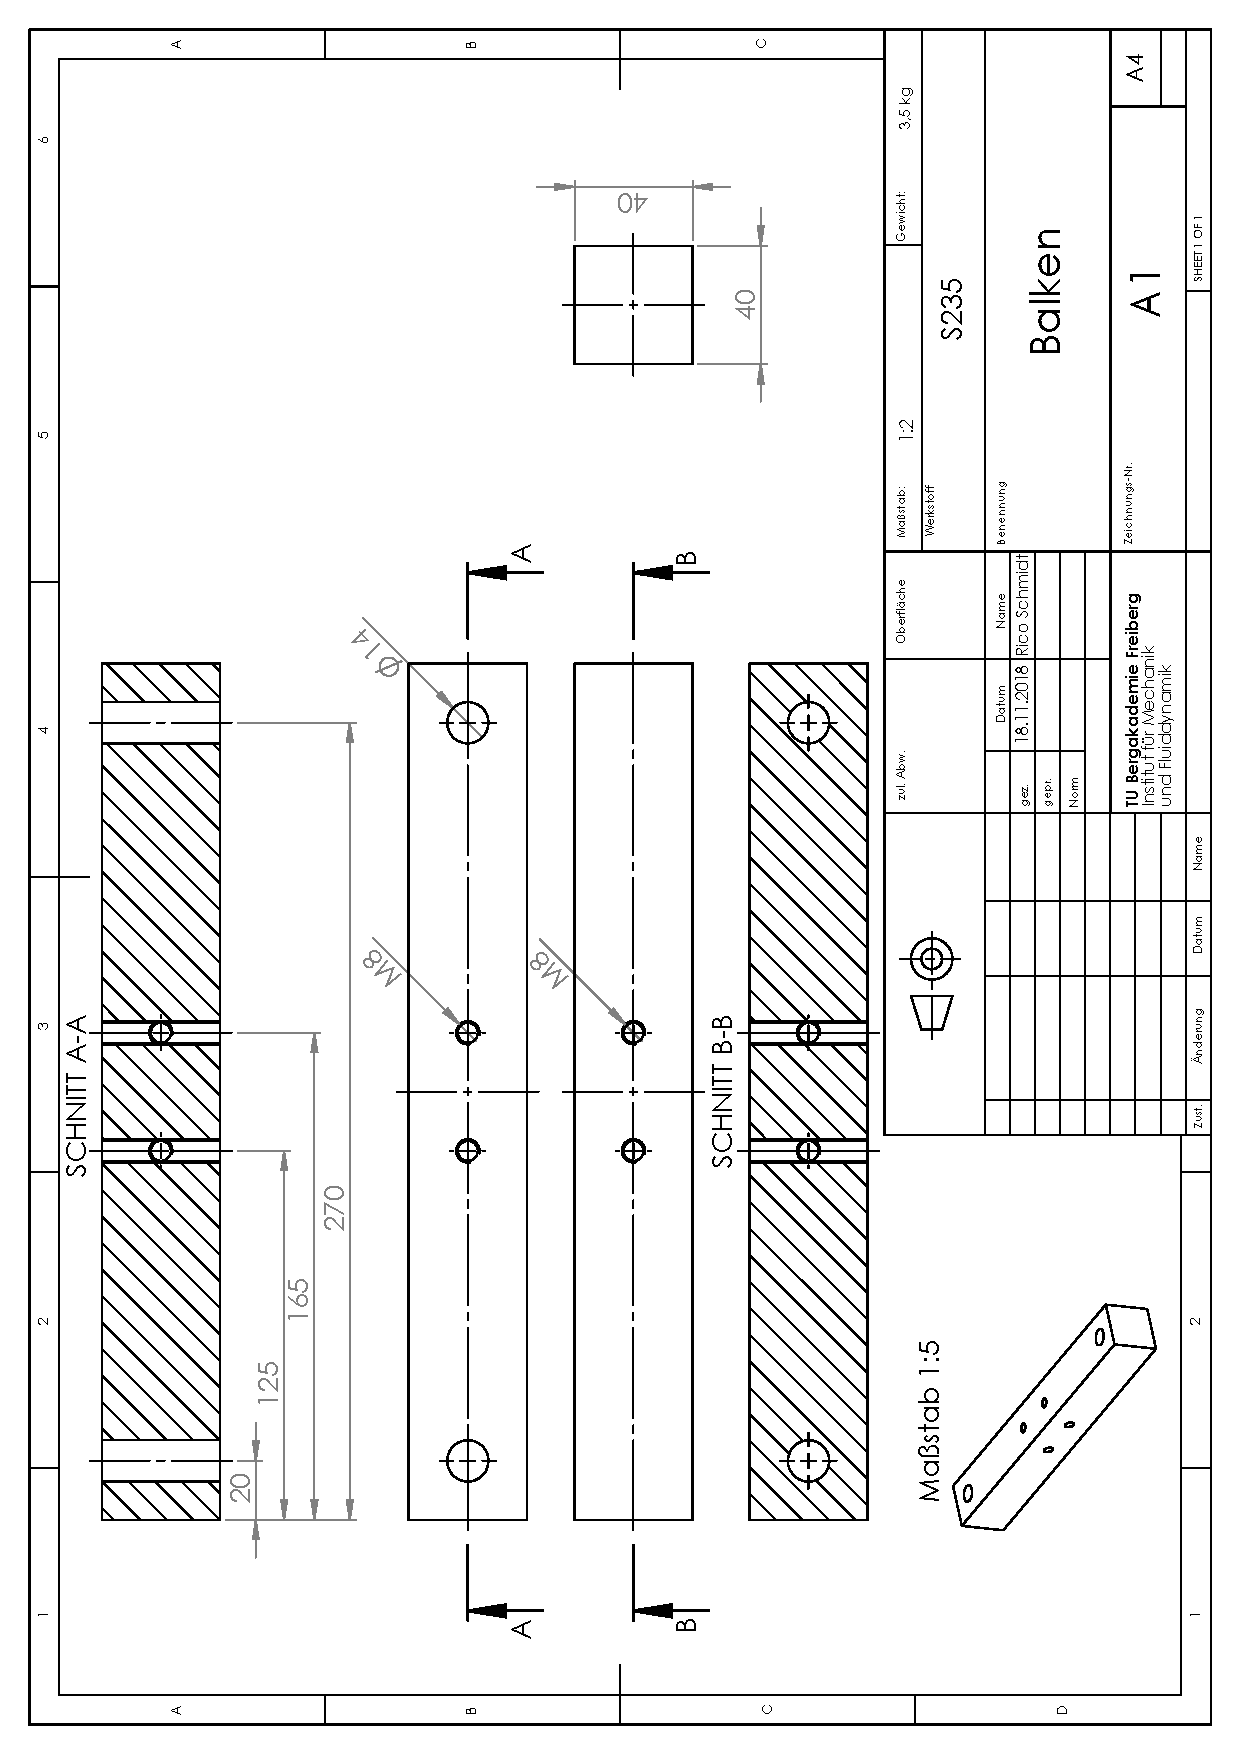
\includegraphics[angle=-90,width=1.0\textwidth]{Anhang/PDFs/Balken}
	
	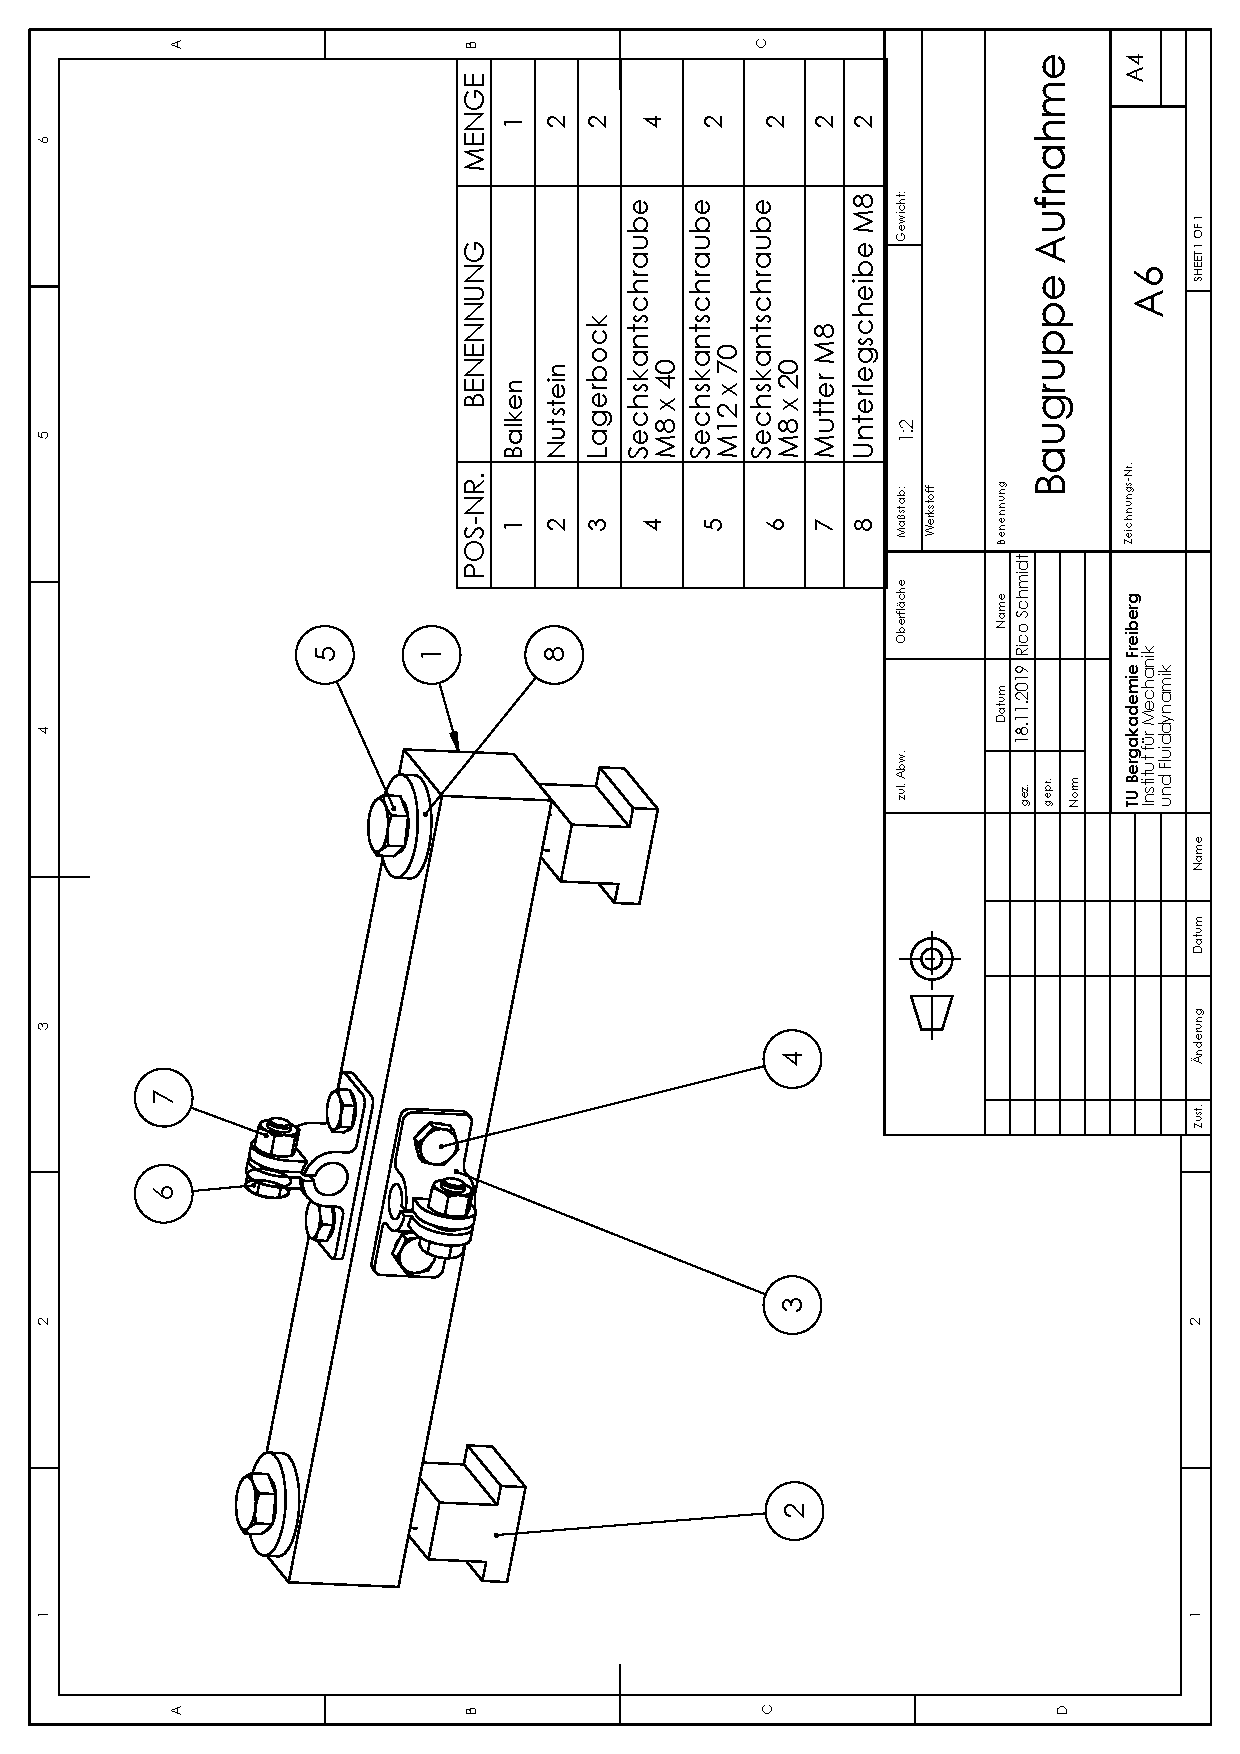
\includegraphics[angle=-90,width=1.0\textwidth]{Anhang/PDFs/Baugruppe_Aufnahme}
	
	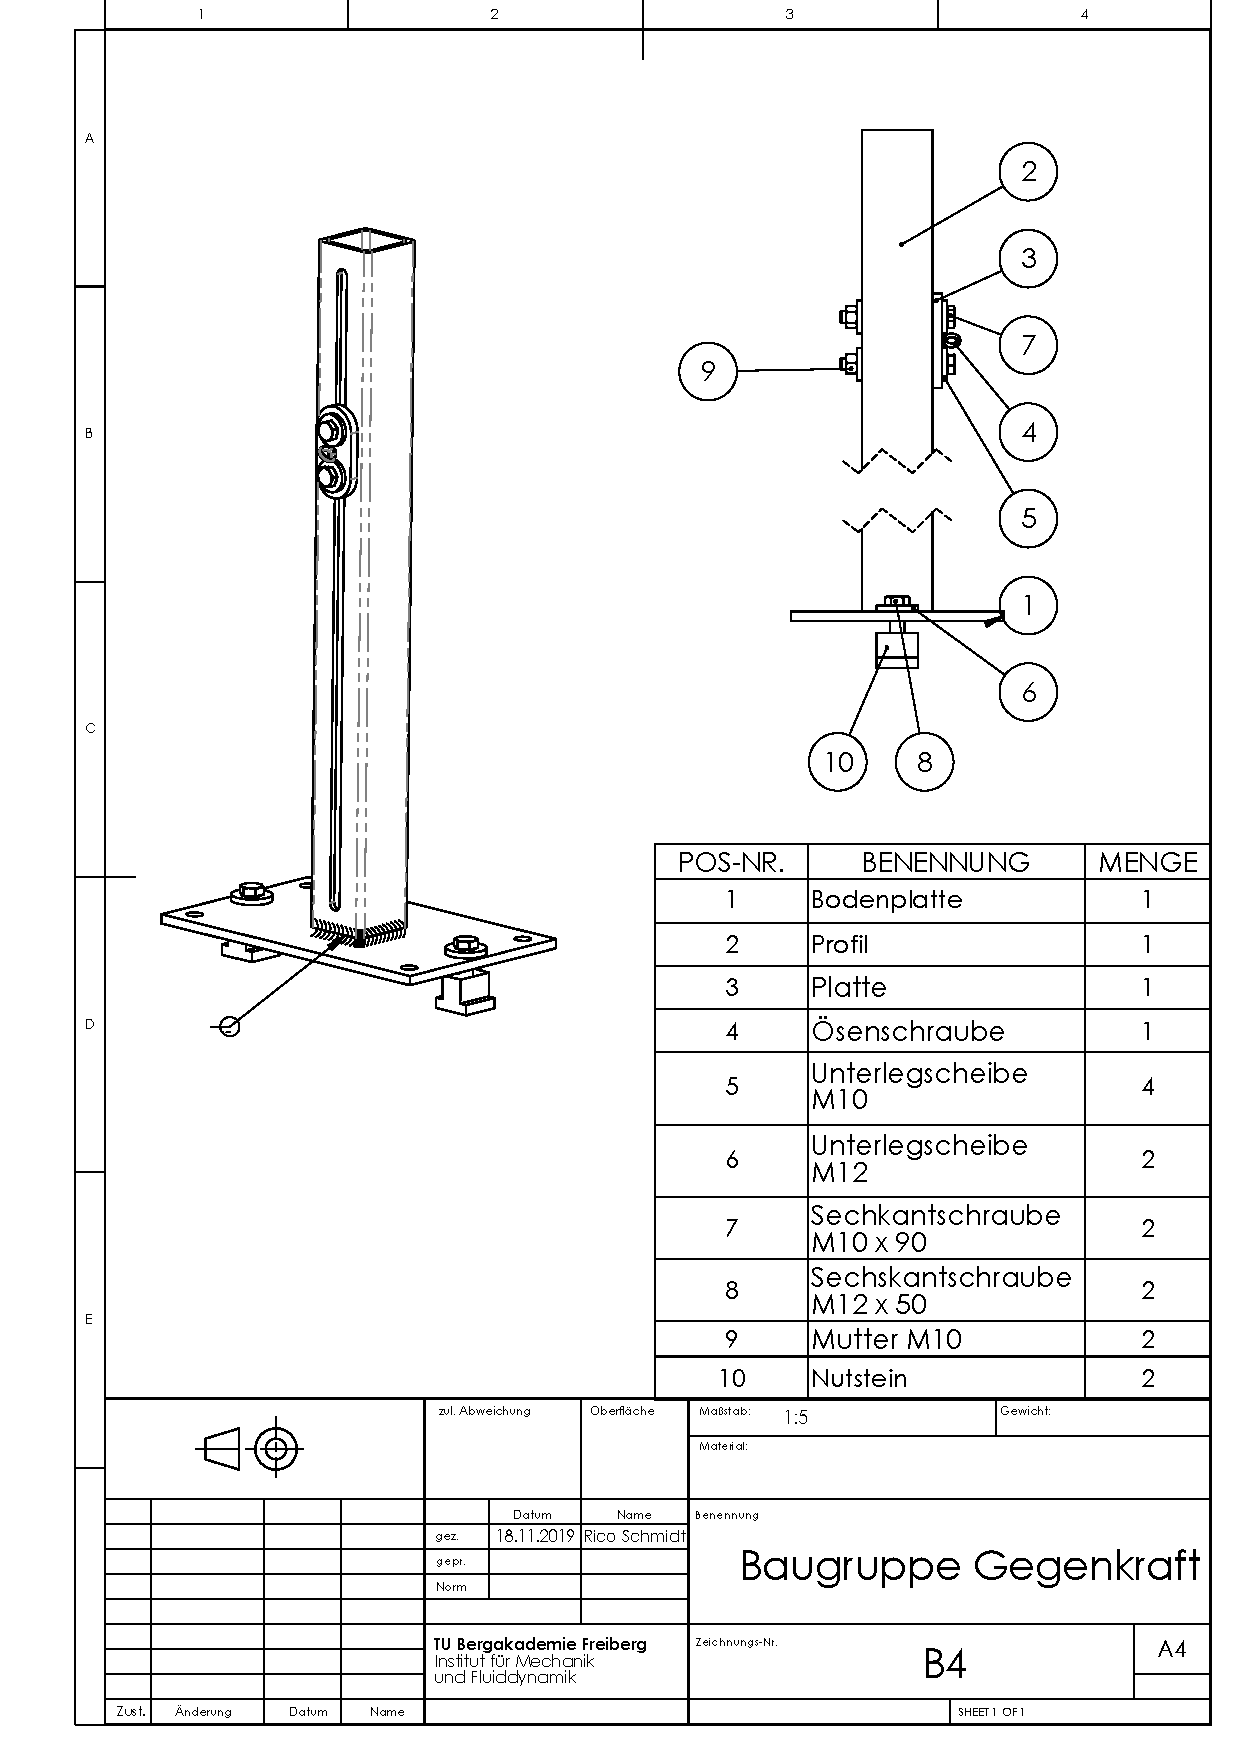
\includegraphics[angle=-90,width=1.0\textwidth]{Anhang/PDFs/Baugruppe_Gegenkraft}
	
	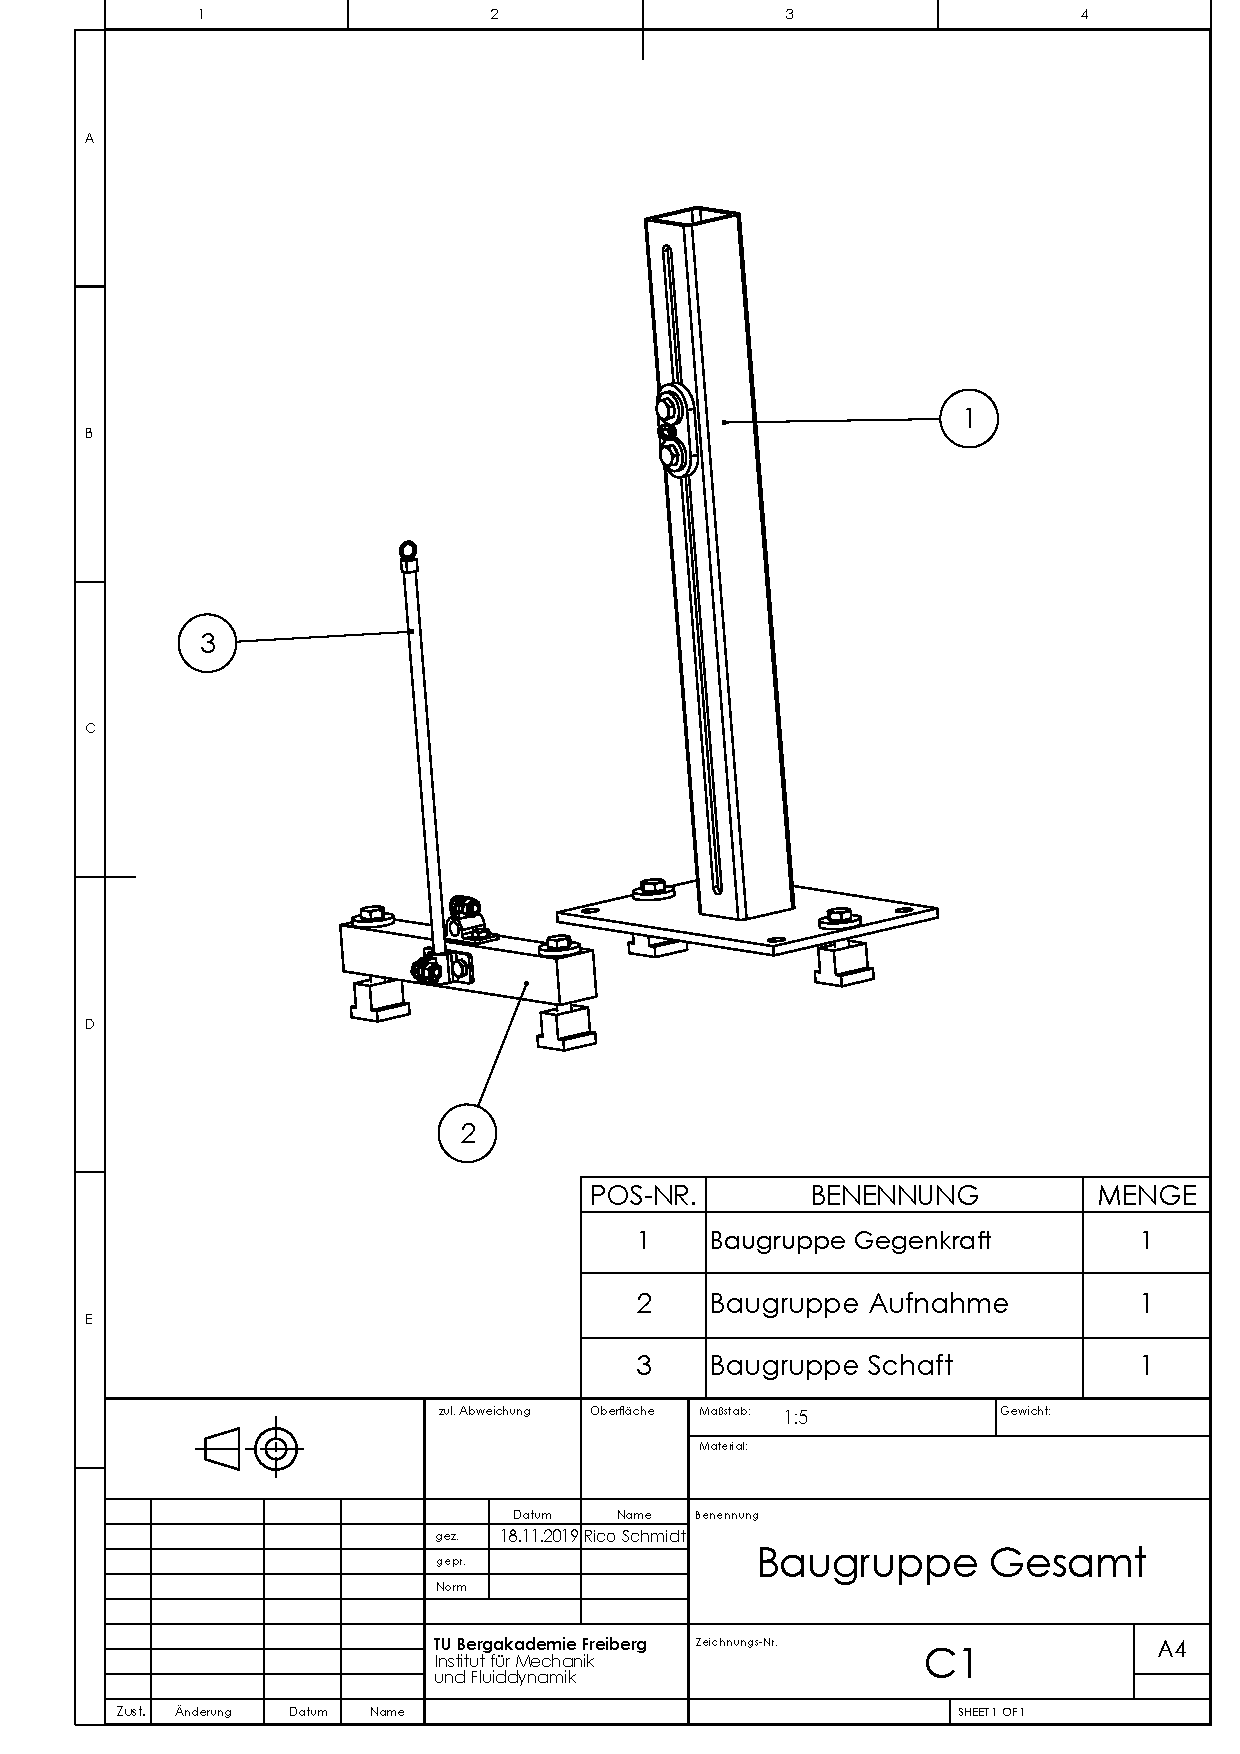
\includegraphics[angle=-90,width=1.0\textwidth]{Anhang/PDFs/Baugruppe_Gesamt}
	
	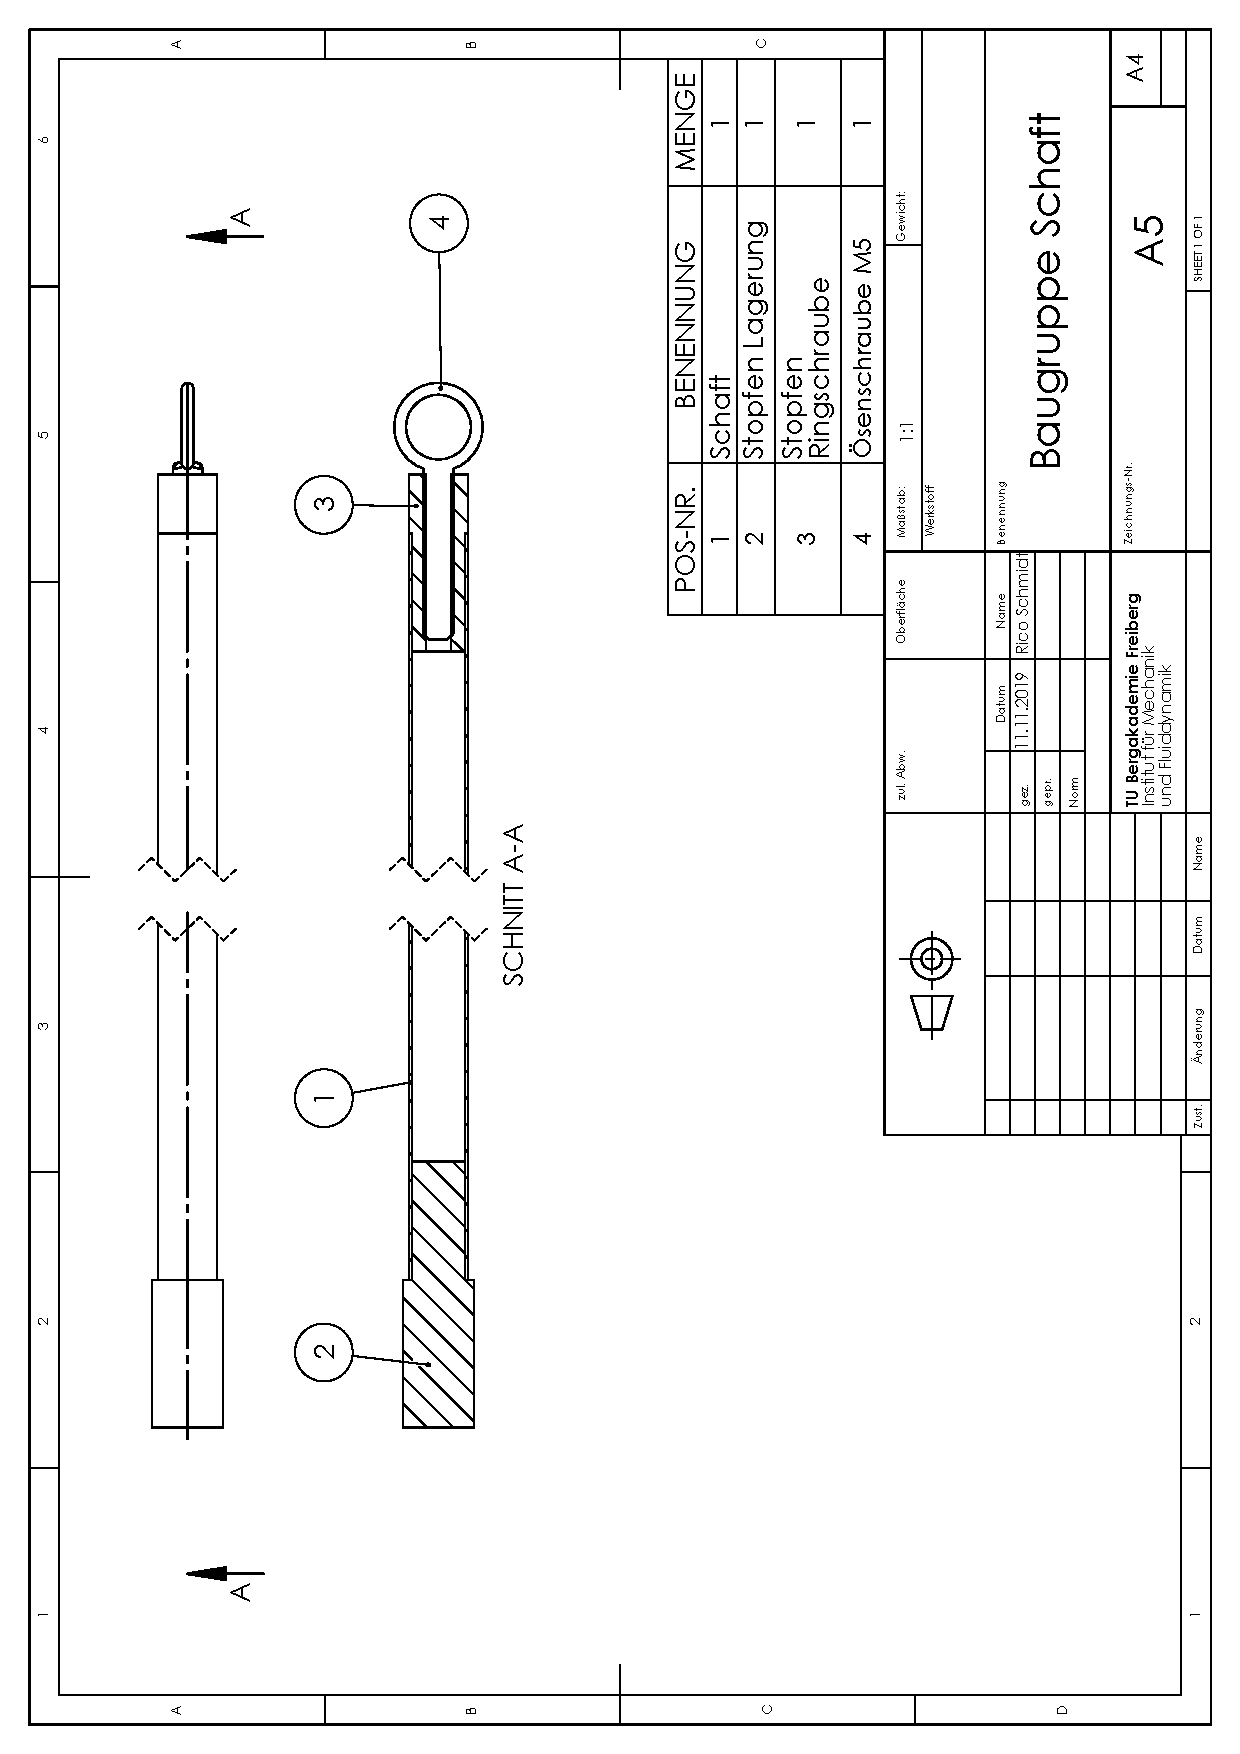
\includegraphics[angle=-90,width=1.0\textwidth]{Anhang/PDFs/Baugruppe_Schaft}
	
	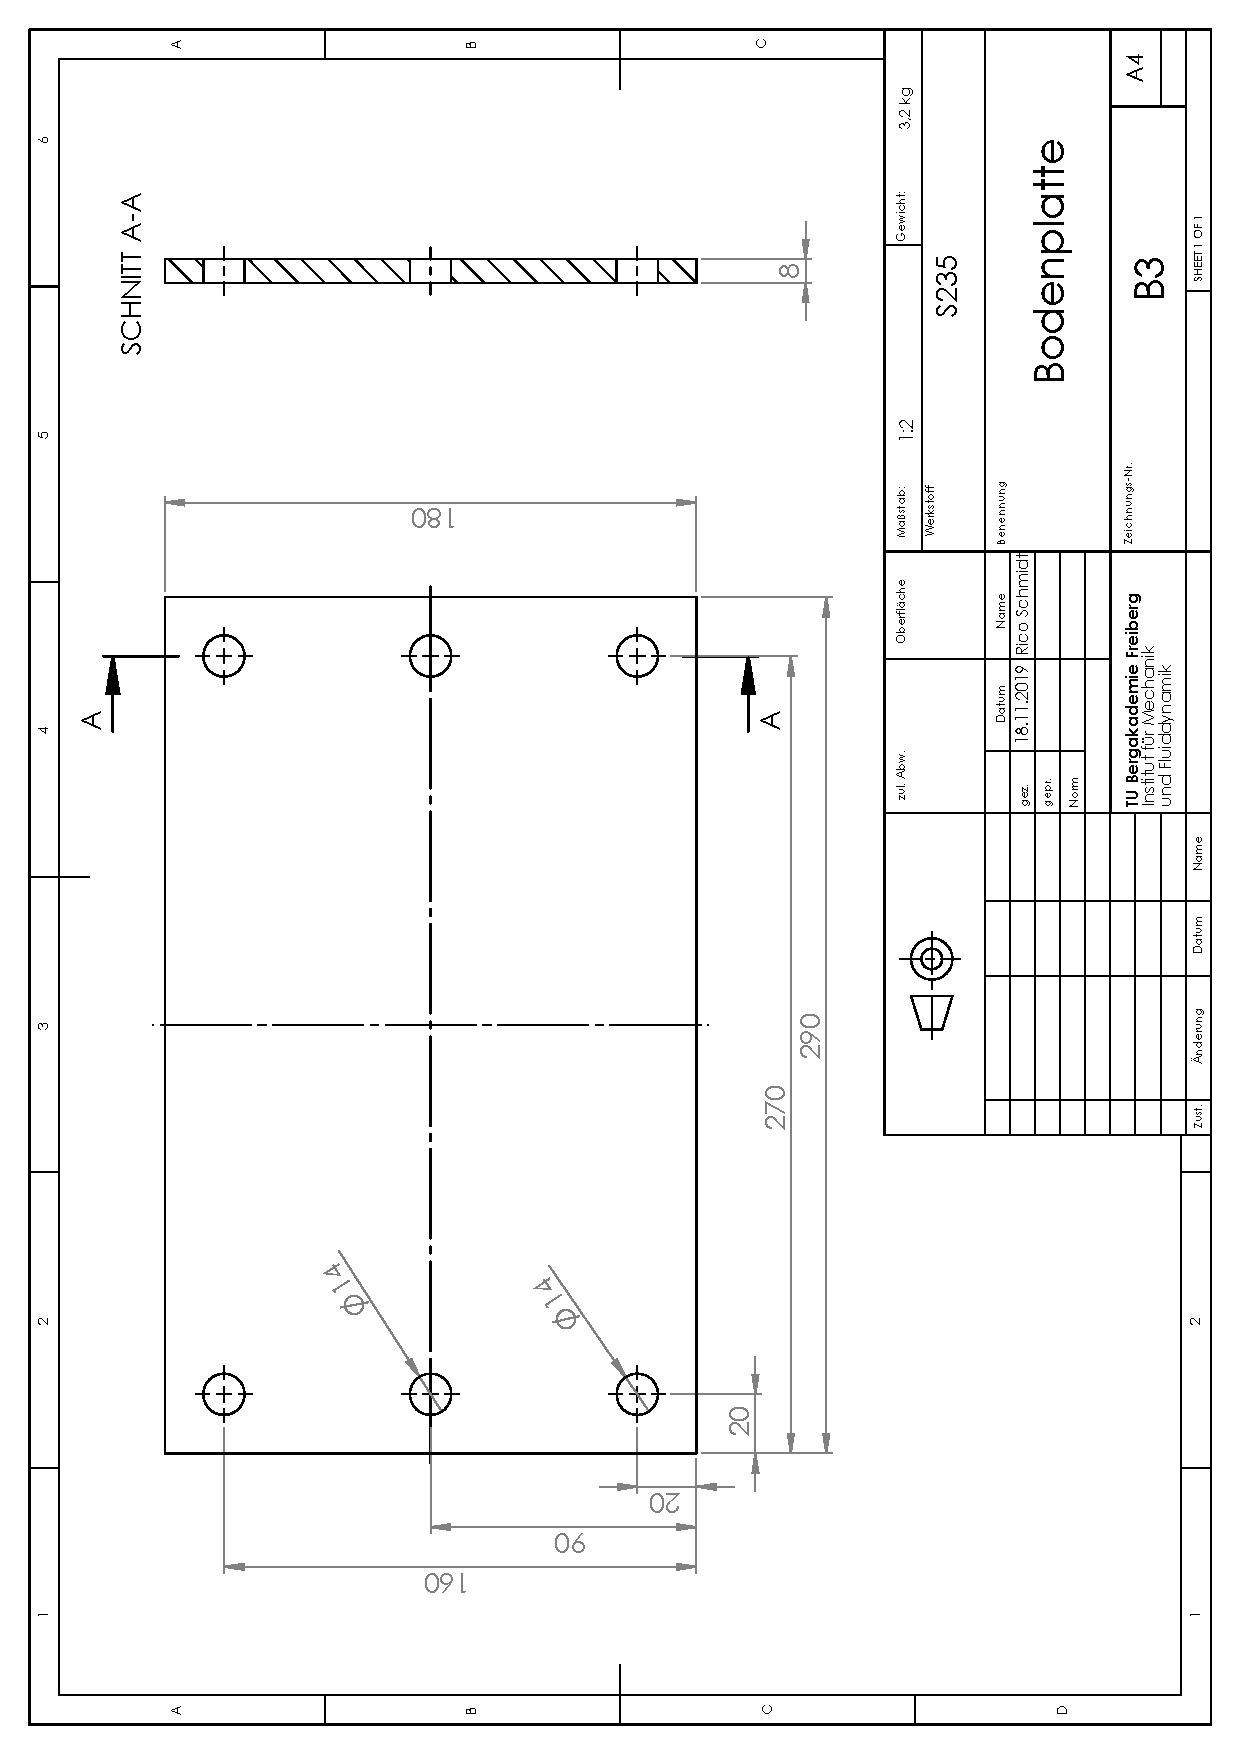
\includegraphics[angle=-90,width=1.0\textwidth]{Anhang/PDFs/Bodenplatte}
	
	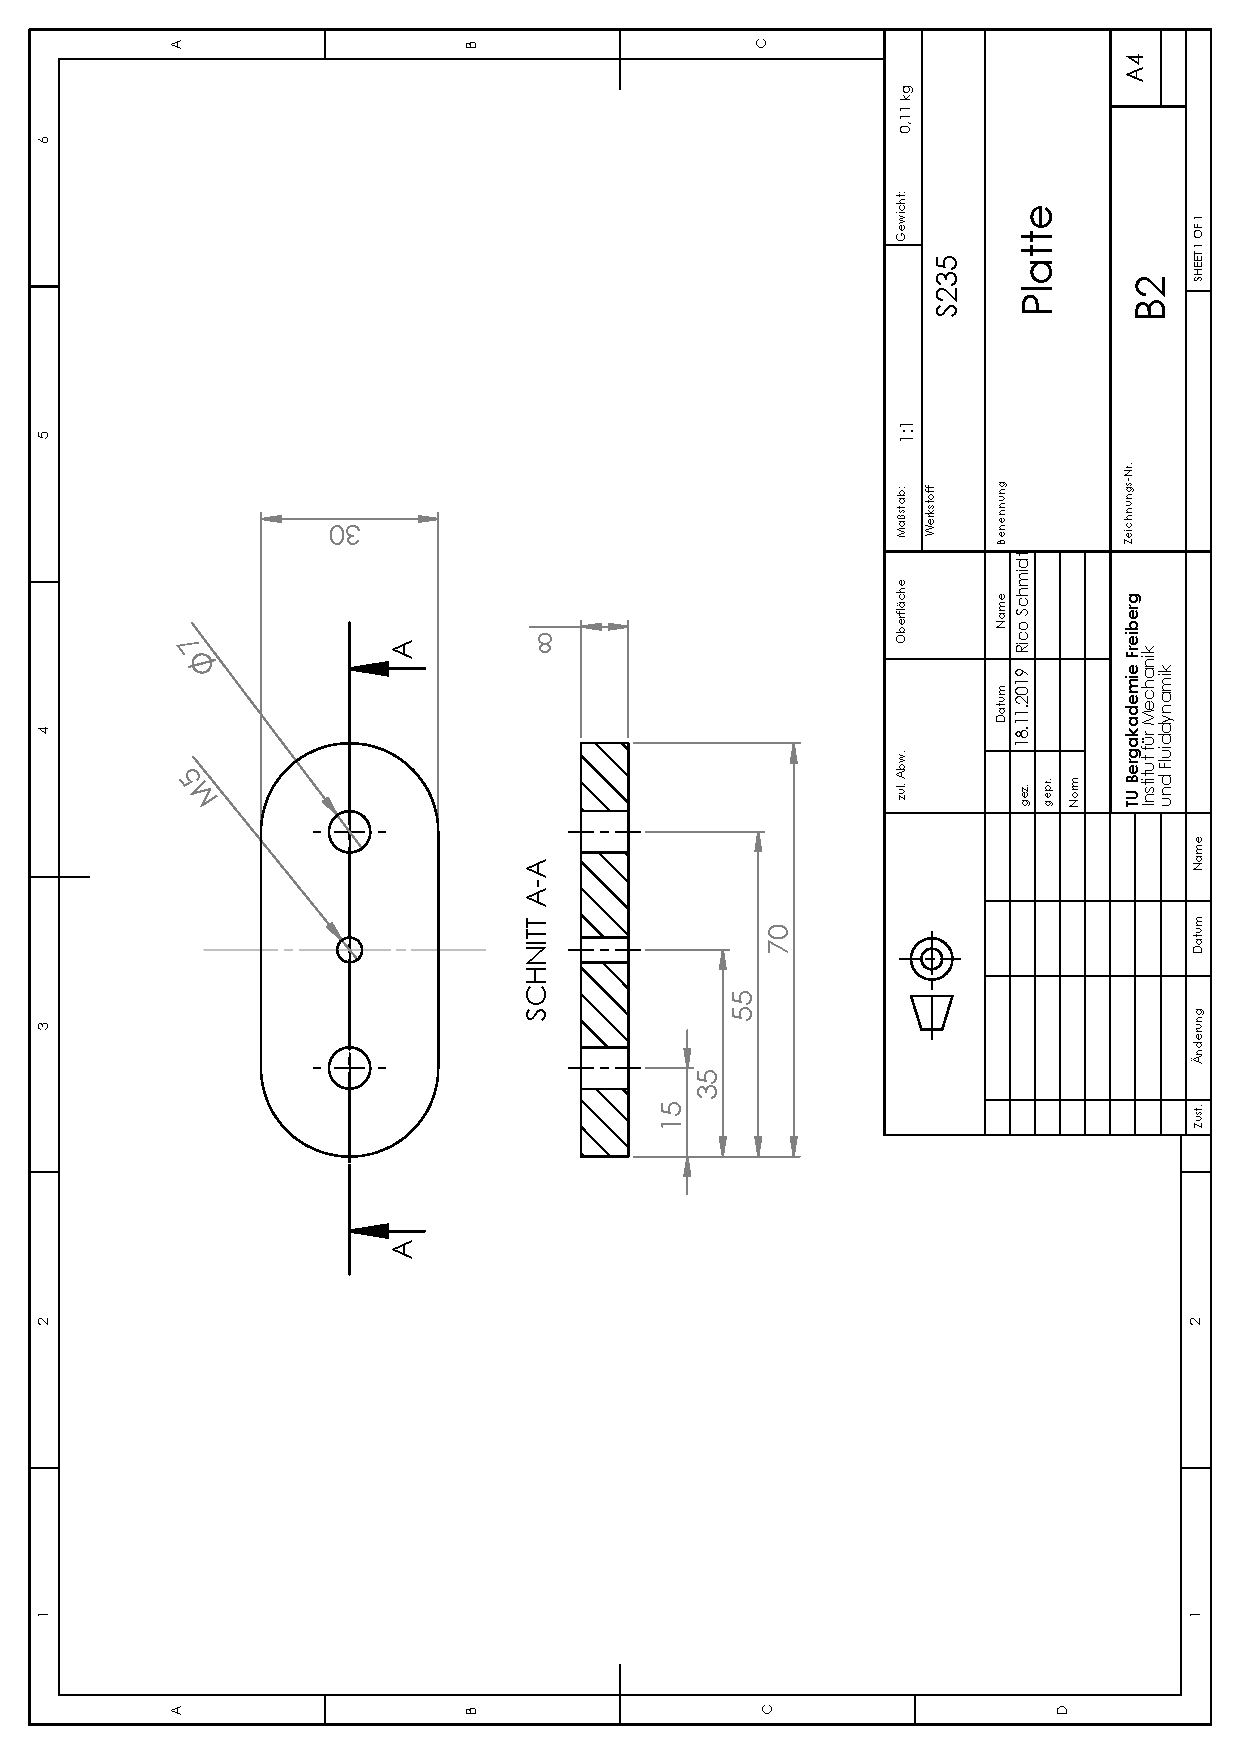
\includegraphics[angle=-90,width=1.0\textwidth]{Anhang/PDFs/Platte_Schlitte}
	
	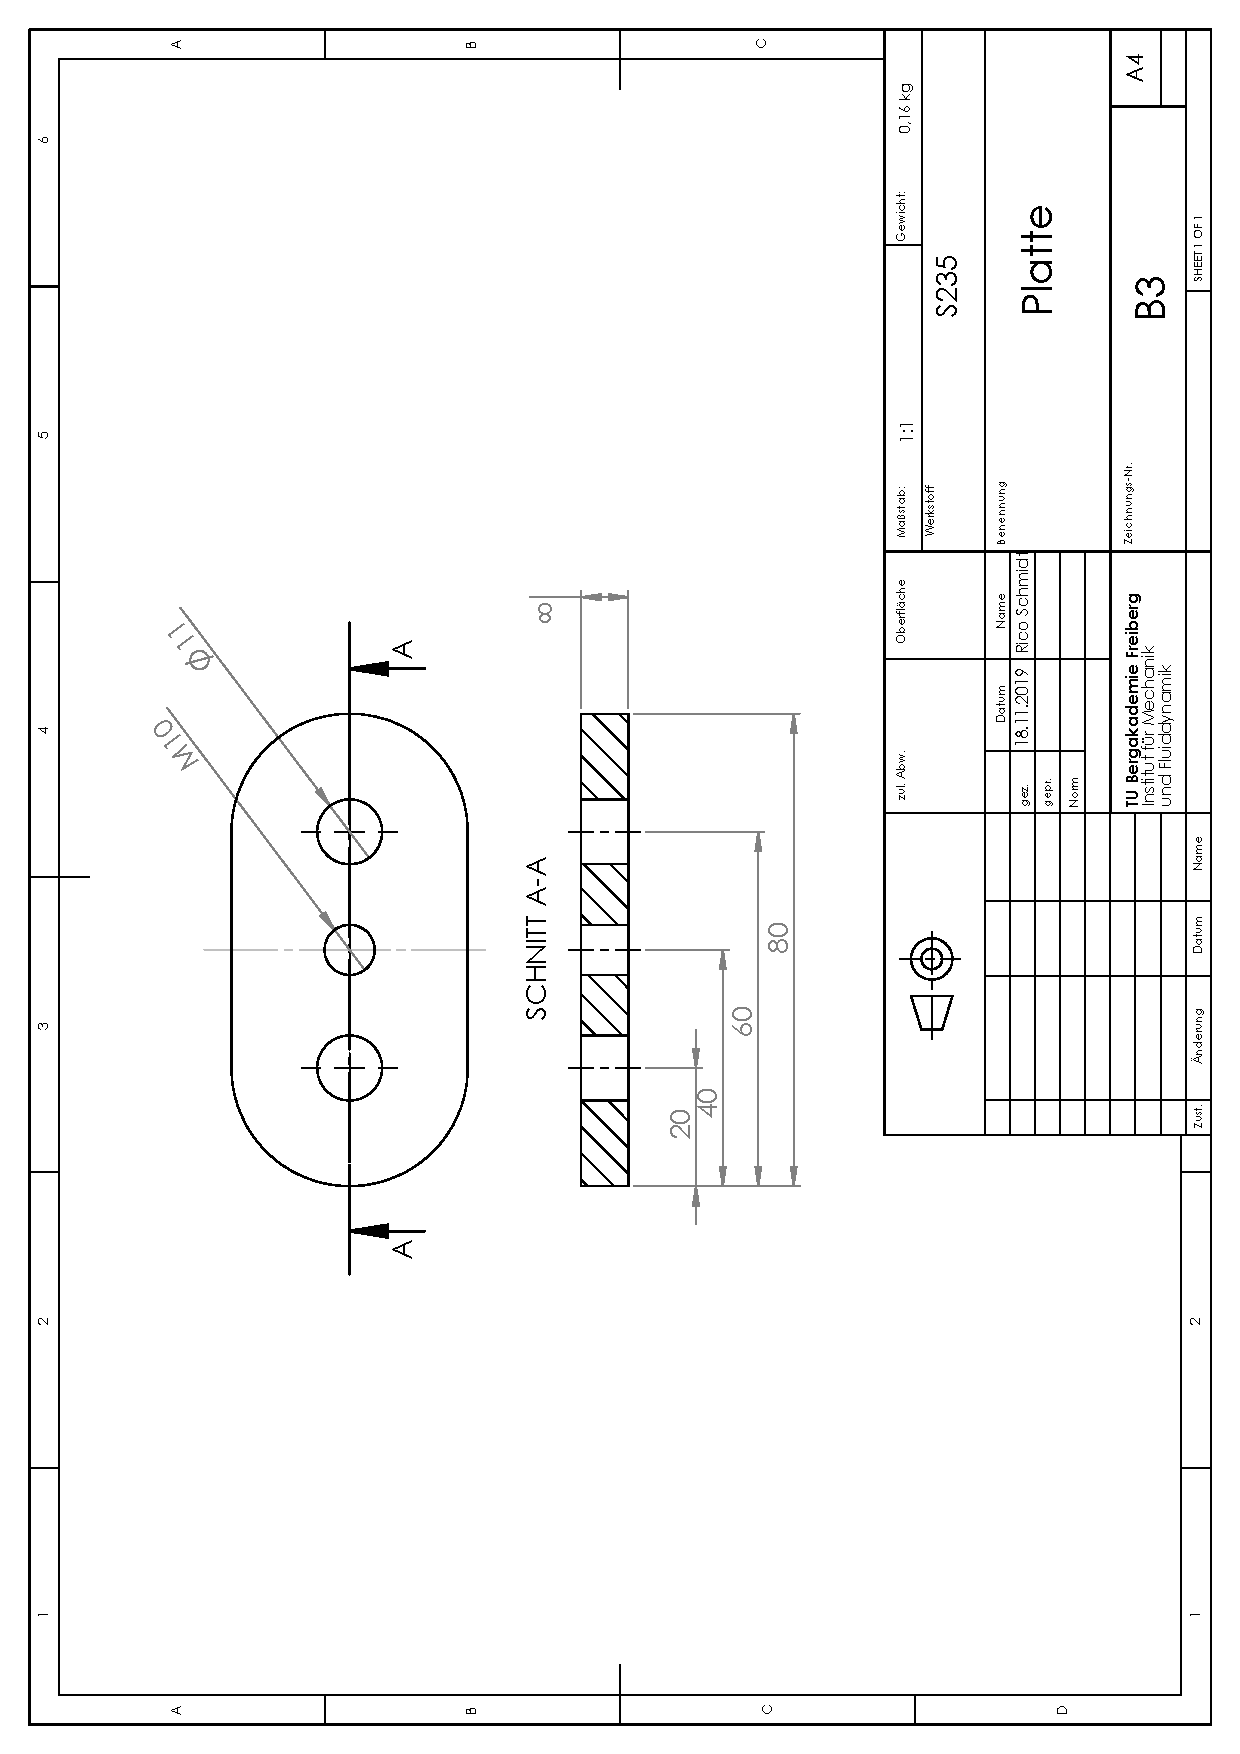
\includegraphics[angle=-90,width=1.0\textwidth]{Anhang/PDFs/Platte_Schlitten}
	
	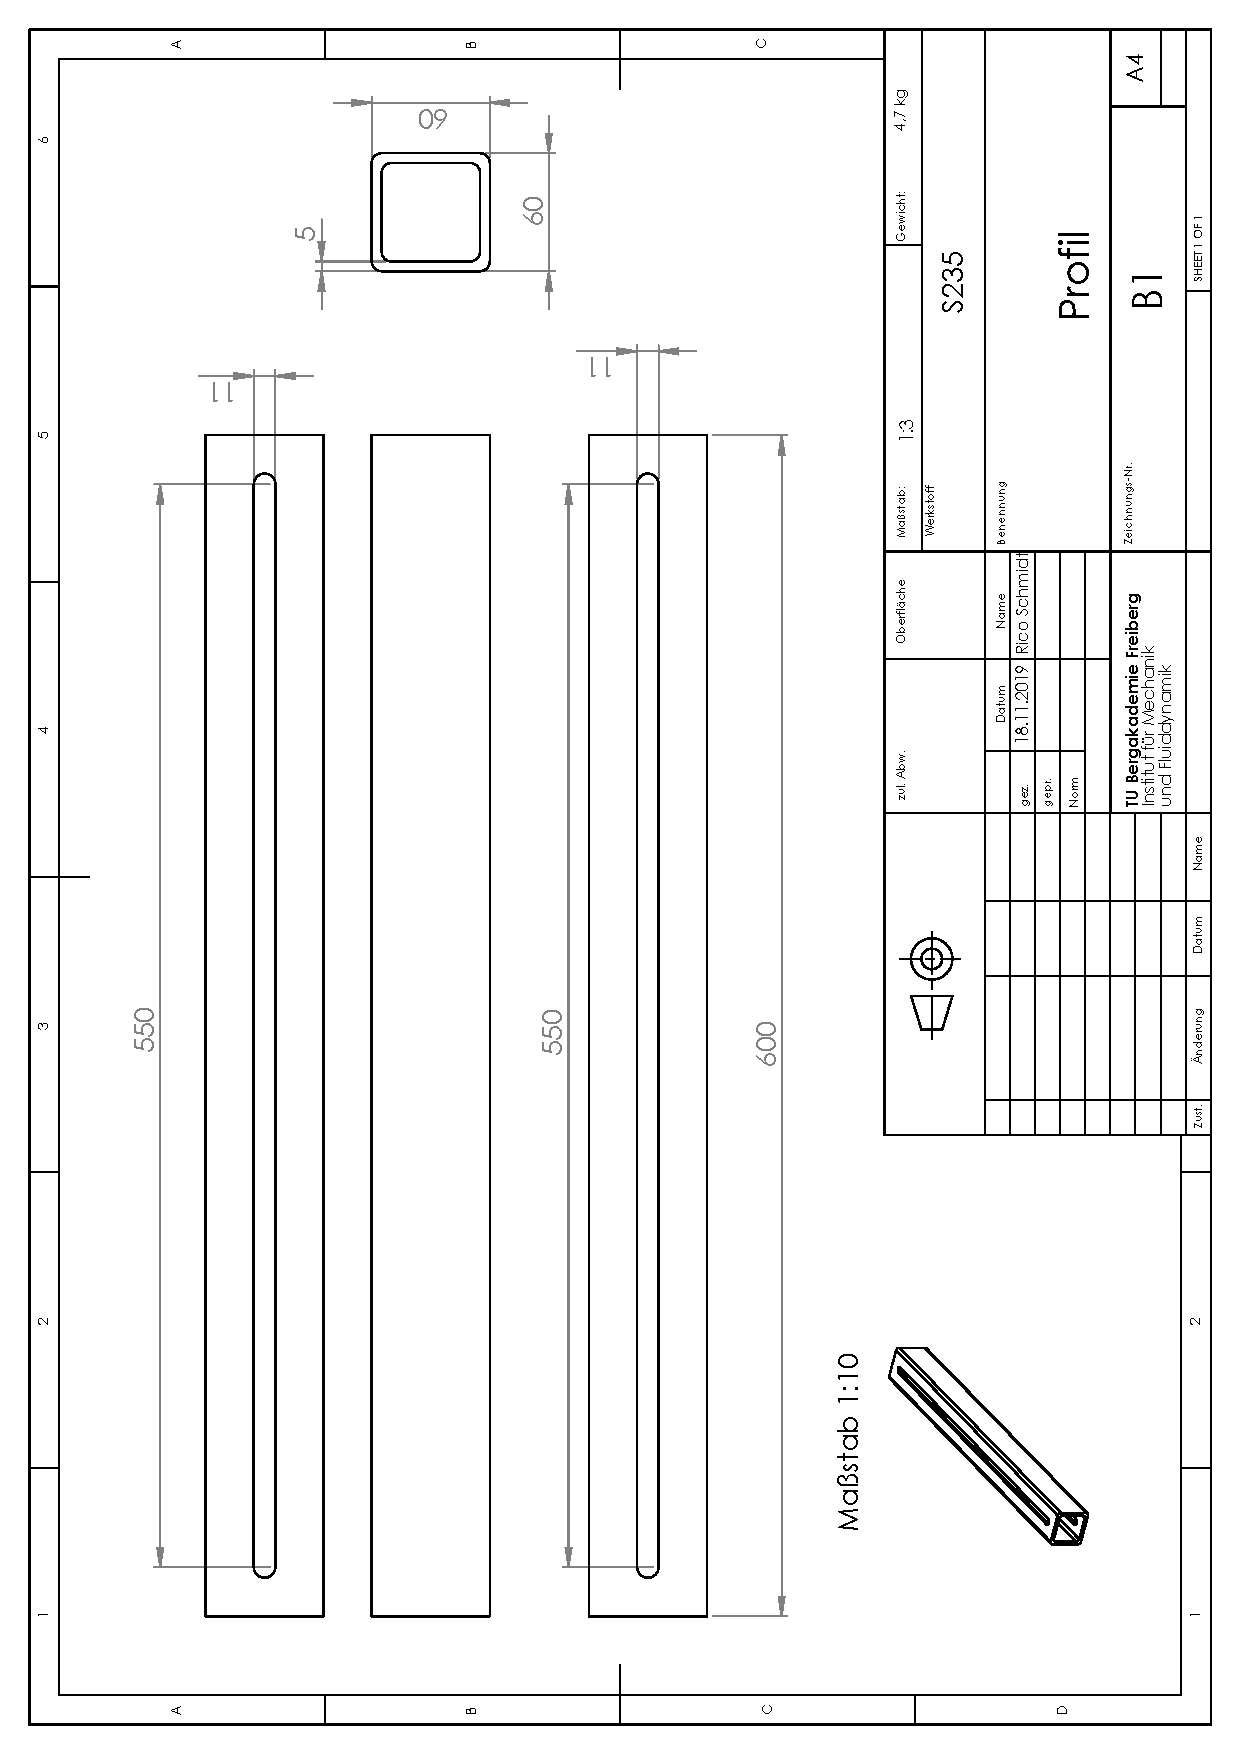
\includegraphics[angle=-90,width=1.0\textwidth]{Anhang/PDFs/Profil}
	
	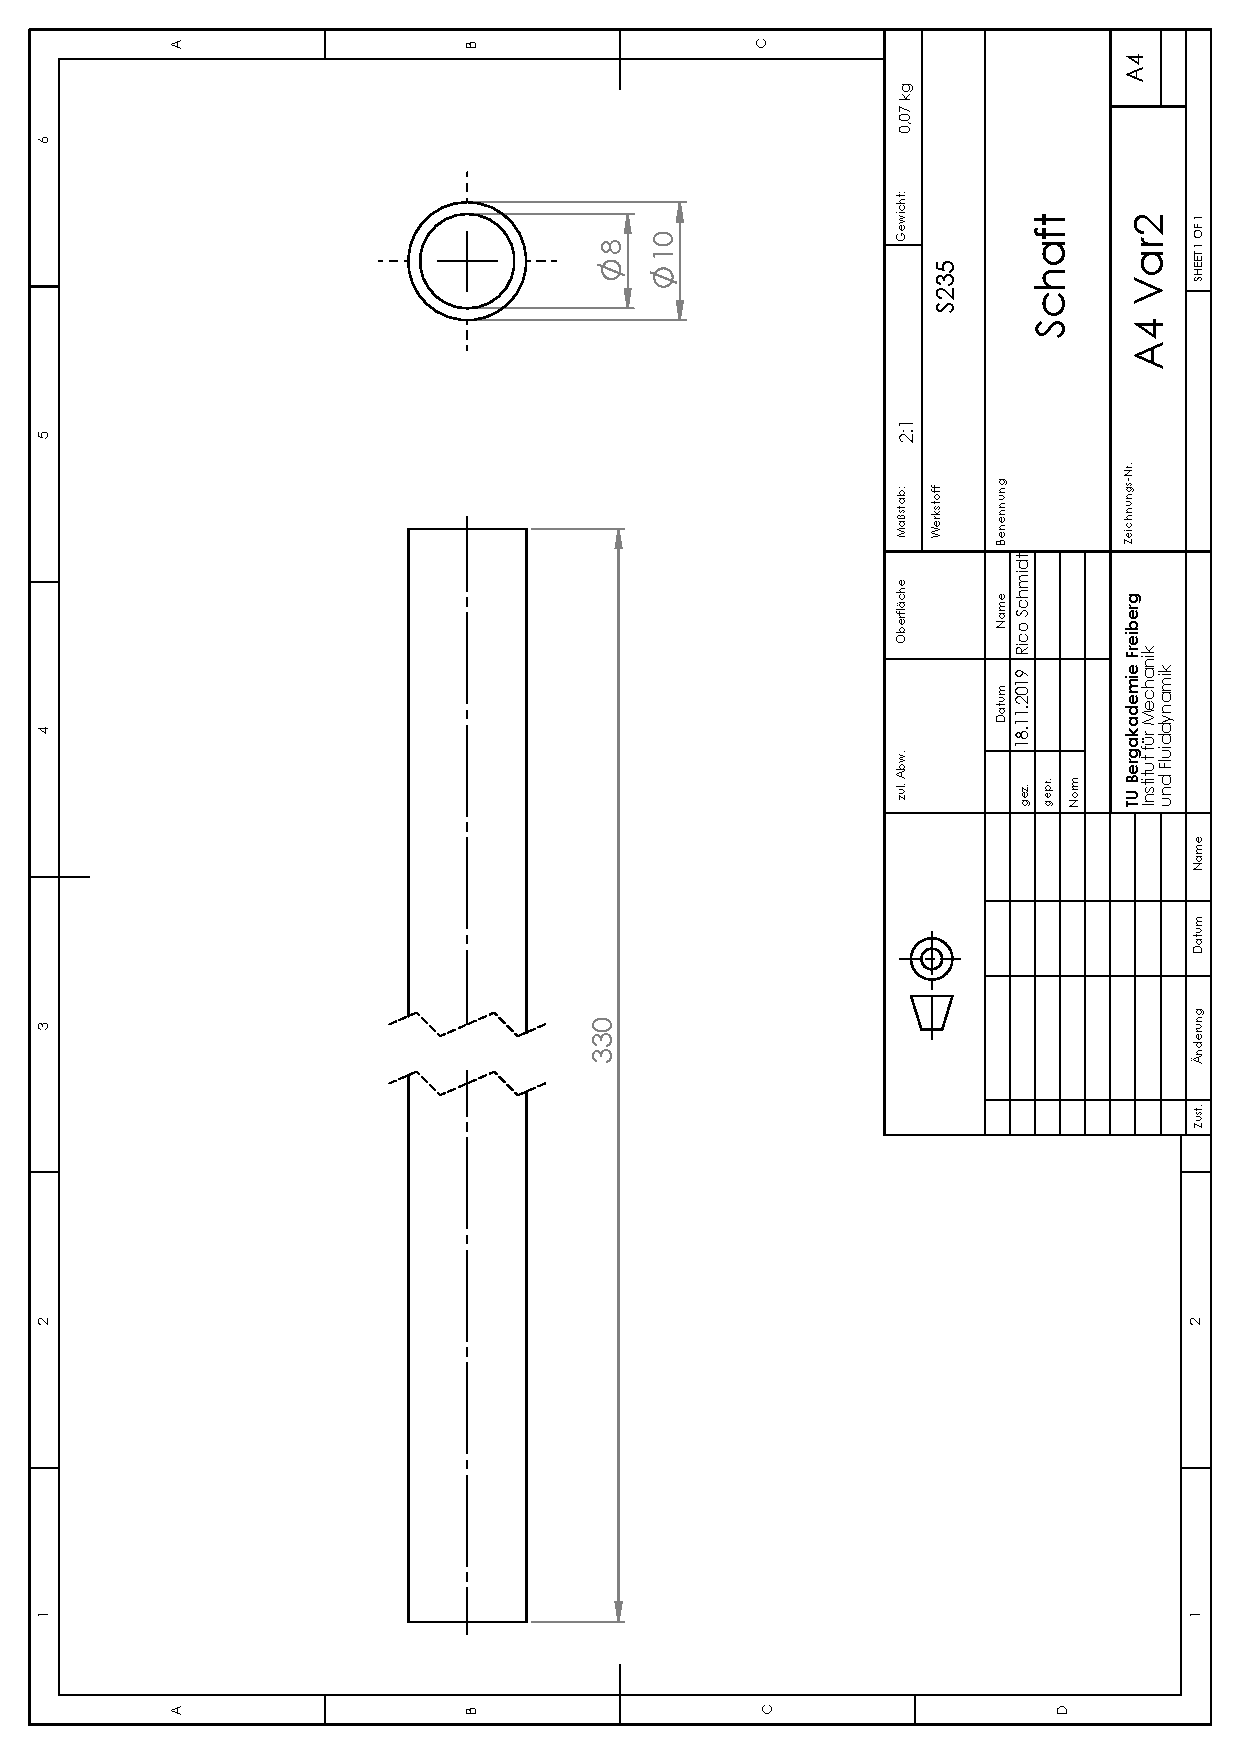
\includegraphics[angle=-90,width=1.0\textwidth]{Anhang/PDFs/Schaft_Ra10mm_Ri8mm}
	
	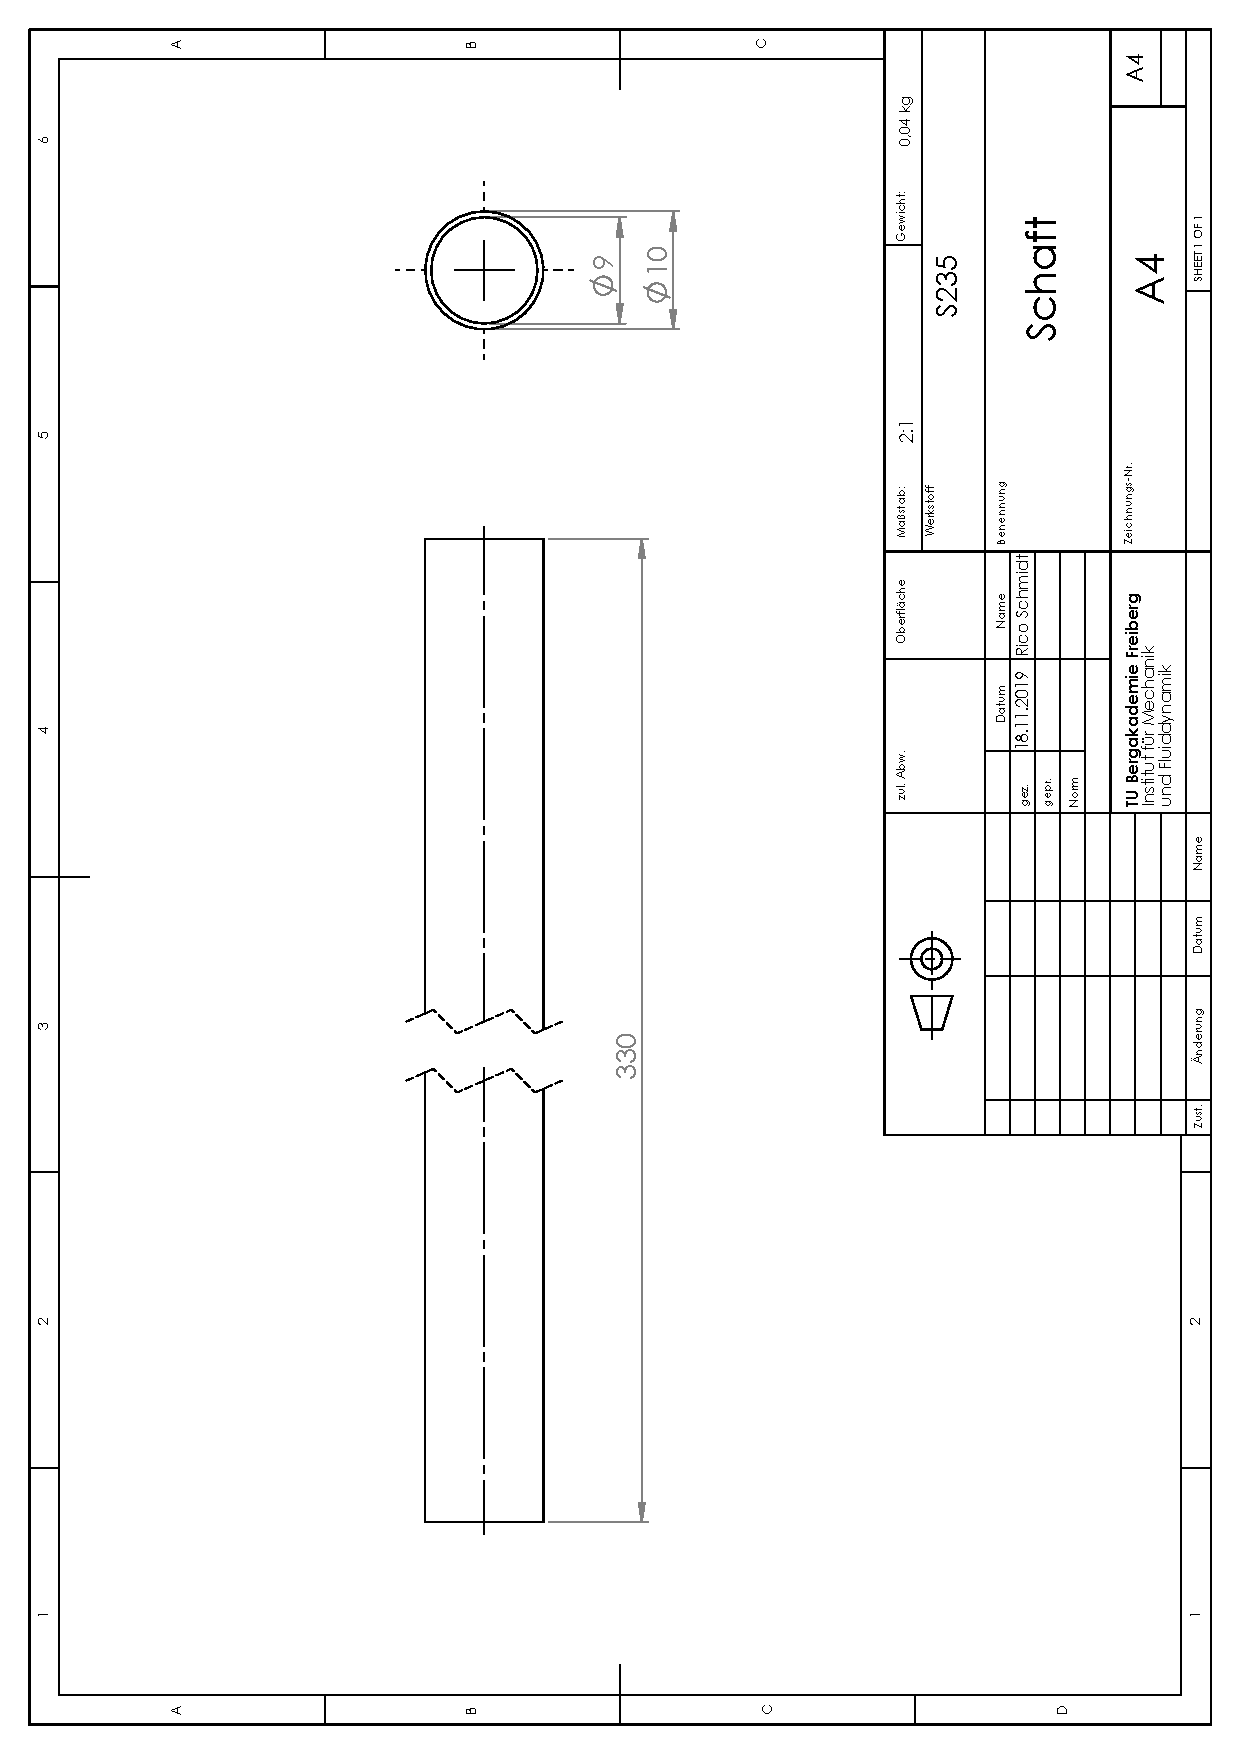
\includegraphics[angle=-90,width=1.0\textwidth]{Anhang/PDFs/Schaft_Ra10mm_Ri9mm}
	
	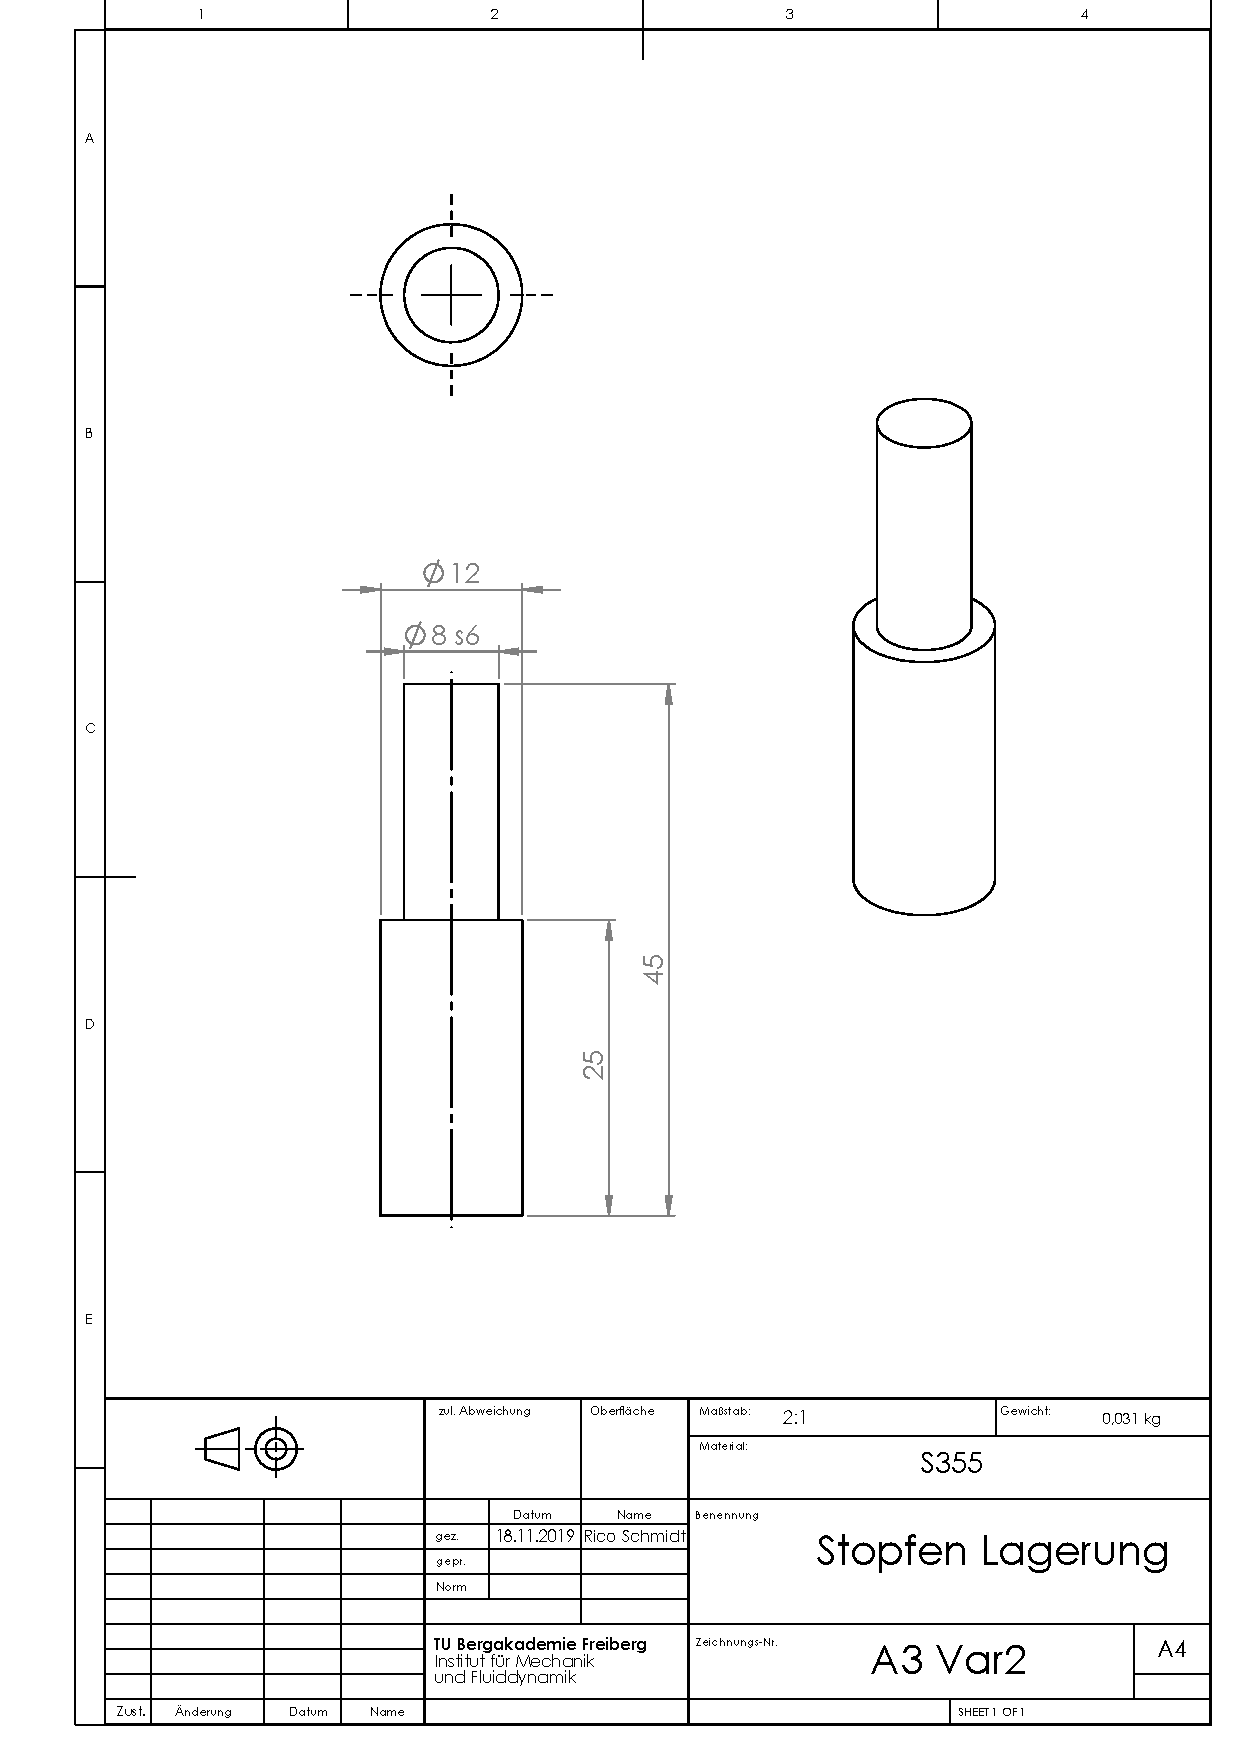
\includegraphics[angle=-90,width=1.0\textwidth]{Anhang/PDFs/Stopfen_Schaft_Lagerung_Var2}
	
	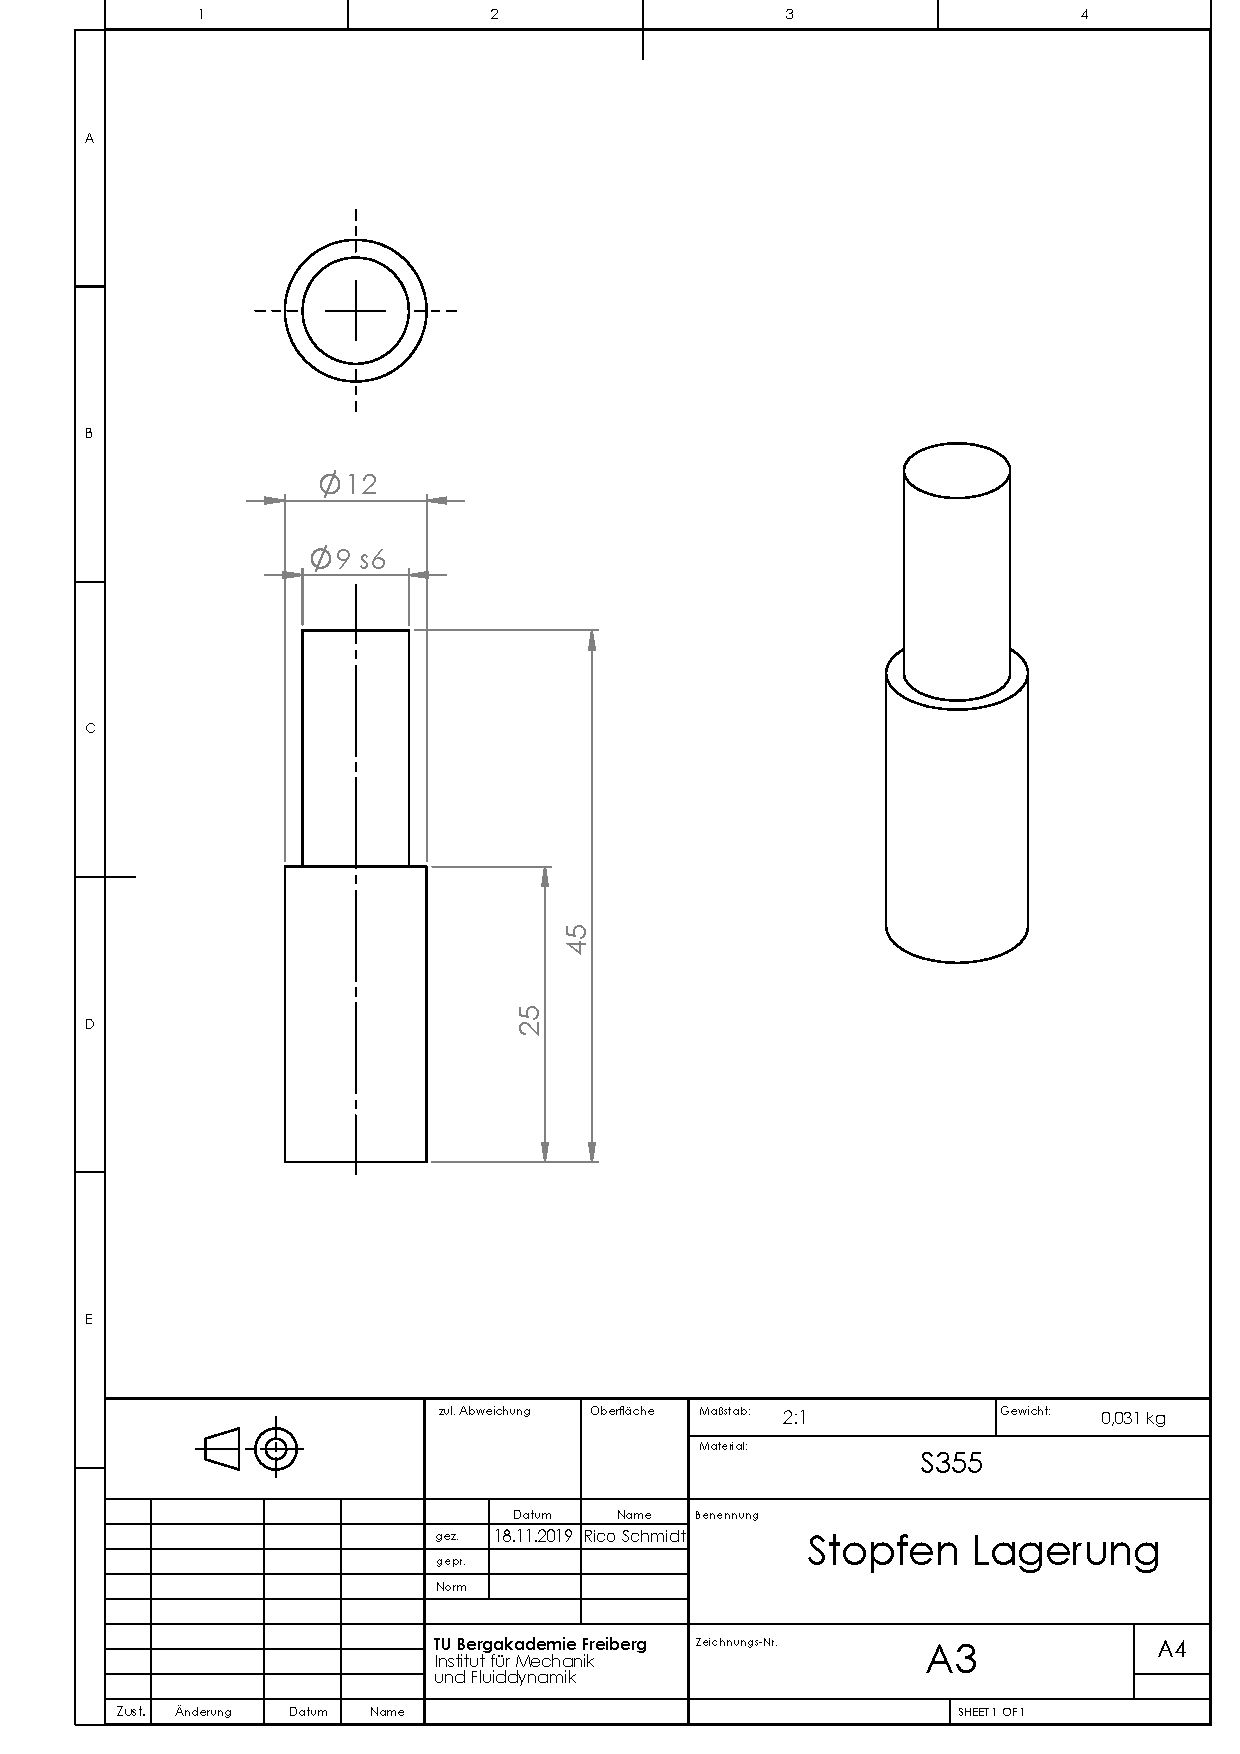
\includegraphics[angle=90,width=1.0\textwidth]{Anhang/PDFs/Stopfen_Schaft_Lagerung}
	
	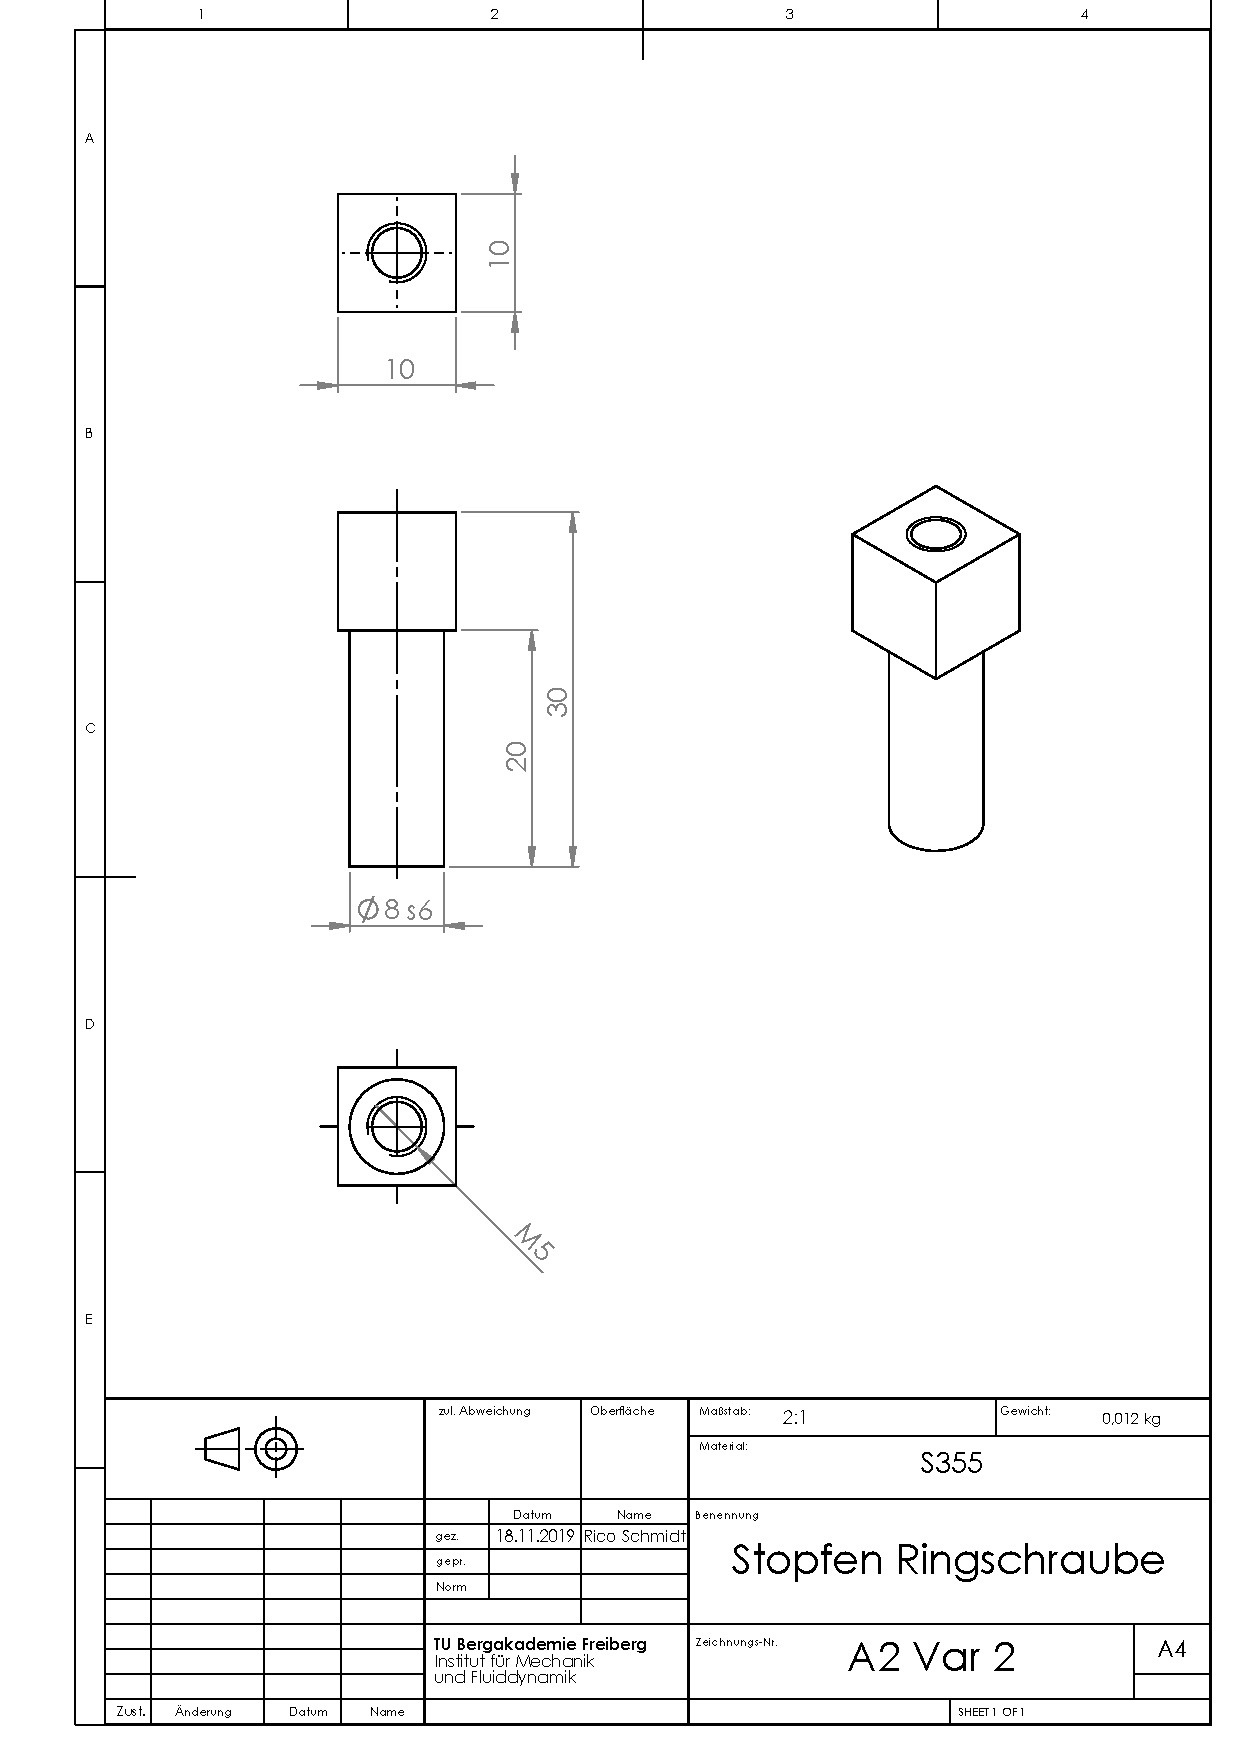
\includegraphics[angle=90,width=1.0\textwidth]{Anhang/PDFs/Stopfen_Schaft_Ringschraube_Var2}
	
	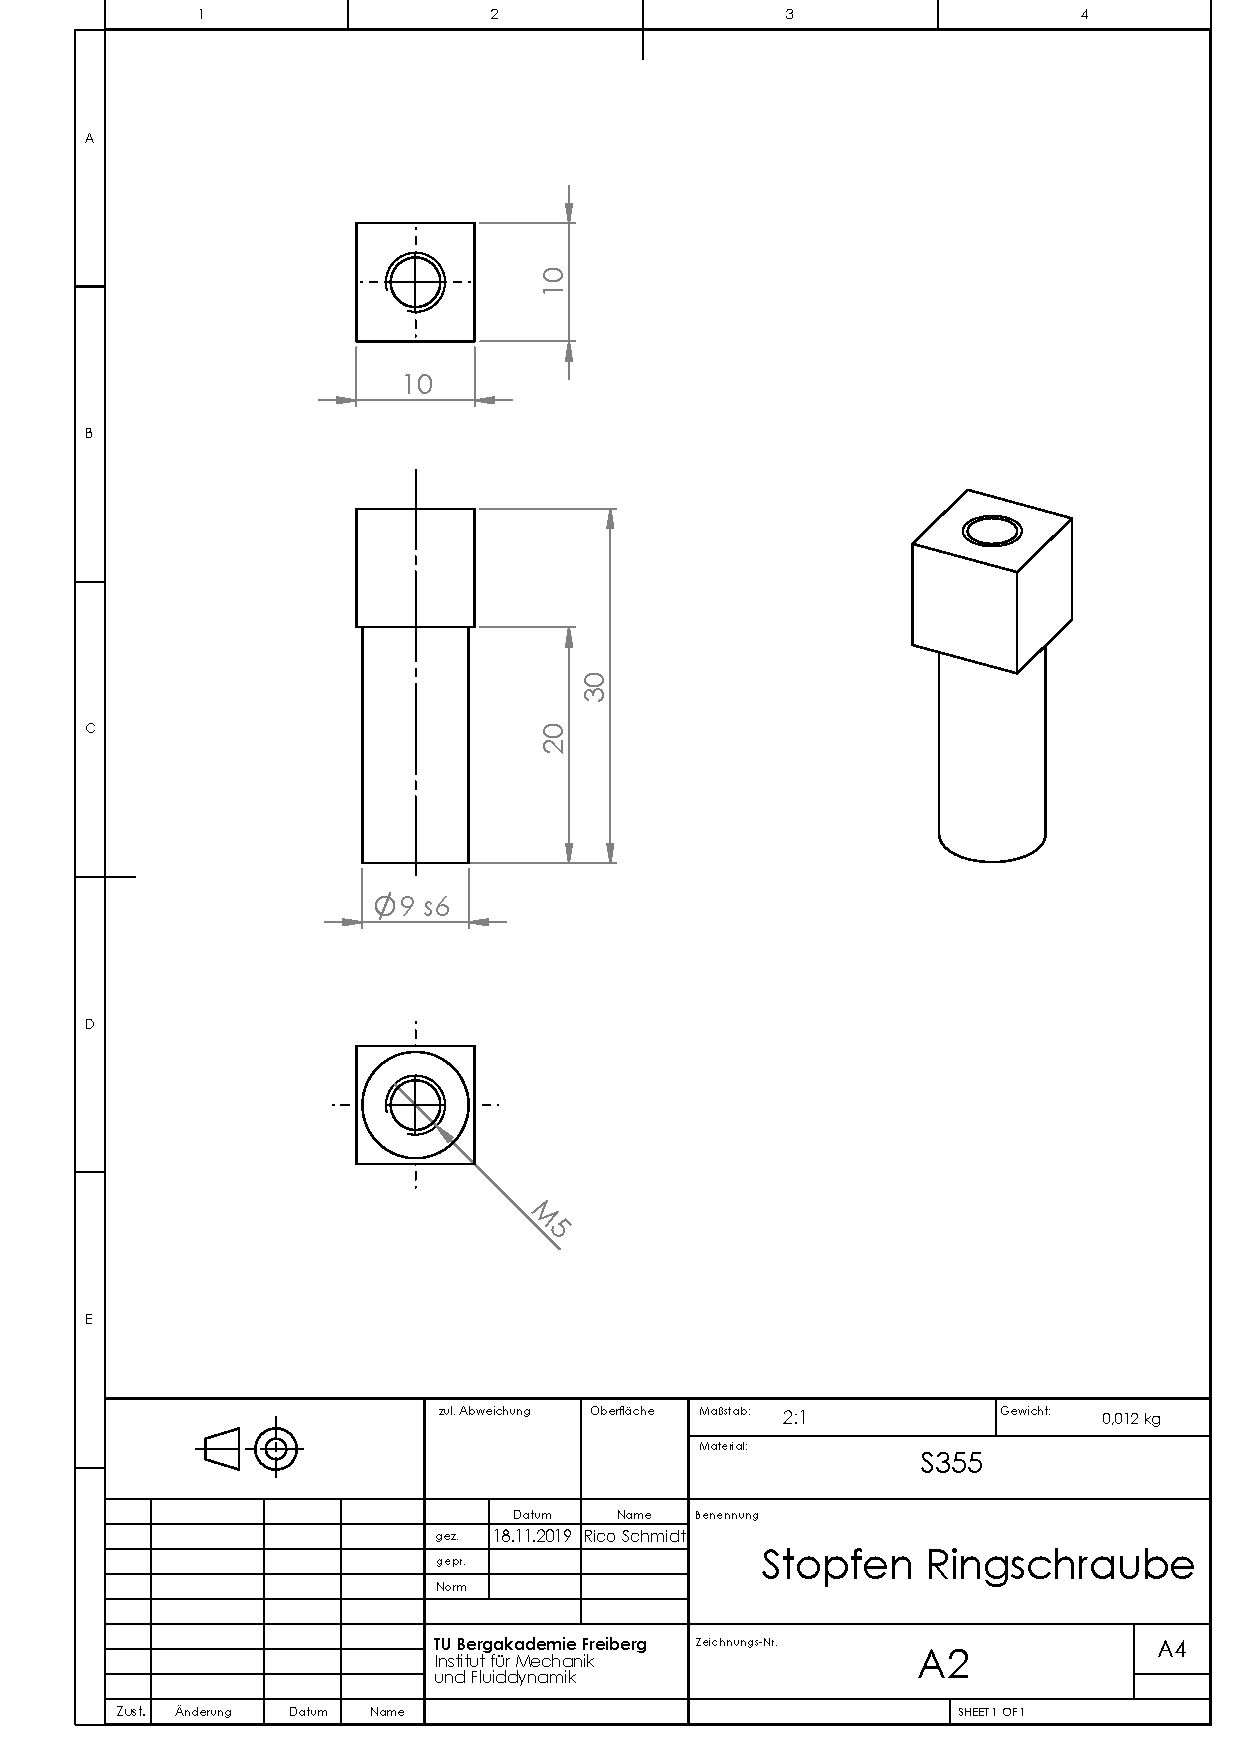
\includegraphics[angle=-90,width=1.0\textwidth]{Anhang/PDFs/Stopfen_Schaft_Ringschraube}
	
	
\end{document}